\todo{Provide table with backgrounds and characteristics...see S Gadatsch thesis Table 5.1 page 126???}

One of the crucial tasks of a physics analysis is to estimate the different background contributions in the SR as accurately as possible.
In this thesis, three different methods are applied for this purpose:
The top quark, \Zjets, and continuum $qqWW$ background (not for the VBF category) are estimated using subsidiary measurements in so-called control regions (CRs), processes with misidentified leptons are estimated using a data-driven method known as the \emph{fake factor method}, and all other background contributions are estimated solely based on simulated samples normalized to the theoretical cross sections for the specific processes.
The following provides an overview of the different estimation strategies, treated separately for each analysis category.

\subsection{Backgrounds estimated with control regions}

- Explain NF method (I guess a formula would be great?)
- CRs defined separately for each analysis category.
- Reference table with all selection criteria.
- Target is to construct regions as pure as possible in a specific background.
- Reference table with pre-fit NFs as well as purities.

- Generally, CRs apply the same SR selections unless mentioned otherwise.

\subsubsection{Continuum $WW$ backgrounds}
The $qqWW$ background is controlled with CRs separated from the SRs using modified selections on the \mll\ observable and purified with additional selections specific to each analysis category.

In the \ZeroJet $WW$ CR, a requirement of $55 < \mll < 110$\,GeV is applied, where the lower boundary ensures orthogonality between the $WW$ CR and the \ZeroJet\ SR, and the upper boundary reduces the contamination from top-quark processes.
In addition, compared to the SR selection, the \DPhill selection is relaxed to $\DPhill < 2.6$, rejecting the majority of \Ztautau processes while retaining many of the $qqWW$ events.
The $WW$ CR in the \OneJet\ category is defined with modified selections: $\mll > 80\,$GeV and $|m_{\tau\tau} - m_Z > 25|\,$GeV, which ensure orthogonality as well as a region pure in $qqWW$ events.
The \TwoJet categories suffer from a large contribution of top-quark processes, which makes it difficult to define regions pure in $WW$ processes.
For the ggF-enriched \TwoJet category, a CR is nonetheless found by requiring $\mll > 80\,$GeV and $\mTtwo > 165\,$GeV. The \mTtwo\ variable is defined as
\begin{equation}
    \mTtwo^2 = \underset{{p\mkern-9.5mu/}_1+{p\mkern-9.5mu/}_2={p\mkern-9.5mu/}_\text{T}}{\textrm{min}} \left[\textrm{max}\{\mt^2(p_\text{T}^a,{p\mkern-9.5mu/}_1),\mt^2(p_\text{T}^b,{p\mkern-9.5mu/}_2)\}\right],
\end{equation}
where the minimization goes over all possible two-momenta, ${p\mkern-9.5mu/}_{1,2}$, such that their sum gives the observed missing transverse momentum ${p\mkern-9.5mu/}_\text{T}$, and where each of $p_\text{T}^a$ and $p_\text{T}^b$ is the combined transverse momentum of a charged lepton and a jet~\cite{PLACEHOLDER:PAPER:CITATION}.
For the VBF-enriched \TwoJet category, no $WW$ CR pure enough in $WW$ processes can be defined.
The $qqWW$ background is therefore estimated from simulated samples normalized to their theoretical cross section.
To validate the consistency between the simulated samples and data, a $WW$ validation region (VR) is used, defined by requiring \todo{WW VR selections}.

\todo{WW VR figure}

\todo{FIGURE}
The purity of the $WW$ process in the CRs as well as the normalization factors are summarized in \cref{table-NFs-purities}.


\subsubsection{Top}
The $t\bar{t}$ and $Wt$ processes are normalized with a combined template using the same NF, extracted from dedicated top-quark CRs.
The relative contribution of $t\bar{t}$ and $Wt$ processes are comparable between the CRs and SRs and its uncertainties are accounted for by treating the relevant sources of uncertainties separately.

The top-quark CRs in the \ZeroJet, \OneJet, and VBF-enriched \TwoJet\ category are defined by requiring the presence of $b$-jets.
For the \ZeroJet\ category, a $b$-jet with $20 < \pT < 30\,$GeV is required.
For the \OneJet\ category, exactly one $b$-jet with $\pT > 30\,$GeV and no $b$-jet with $20 < \pT < 30\,$GeV is required. These specific selections ensure that the ratio between $t\bar{t}$ and $Wt$ processes is similar between the CR and the SR without compromising the purity of top-quark processes in the CR.
The top-quark CR in the VBF-enriched \TwoJet category is defined by requiring the presence of exactly one $b$-jet with $\pT > 30\,$GeV.
In the ggF-enriched \TwoJet\ region, an alternative strategy is used that does not rely on $b$-jet requirements, while still retaining a high purity of top-quark events. The CR is defined by requiring $\mll > 80\,$GeV and $\mTtwo < 165\,$GeV, where the latter selection ensures orthogonality to the $WW$ CR. This definition reduces the uncertainties from flavor tagging selections and is therefore preferable to a CR defined using $b$-jet criteria.

The purity of the $WW$ process in the CRs as well as the normalization factors are summarized in \cref{table-NFs-purities}.

\subsubsection{\Ztautau background}
The \Ztautau\ background is normalized using dedicated CRs, defined separately for each analysis category.
The CR in the \ZeroJet category requires a large opening angle of the leptons of $\DPhill > 2.8$.
For the \OneJet and two \TwoJet categories, the \mtautau observable is exploited to separate the \Ztautau CRs from the SRs by selecting the region around the nominal $Z$ boson mass.
The specific selections are $\mtautau - m_Z < 25\,$GeV for the \OneJet and ggF-enriched \TwoJet category and $|\mtautau - m_Z| \le 25\,$GeV for the VBF-enriched \TwoJet category.

In order to increase the statistical precision of the CRs, some selections made in the SR are relaxed or dropped.
In the \ZeroJet and \OneJet category, no \pTmiss requirement is applied and the \mll\ selection is relaxed to $\mll < 80\,$GeV.
In the VBF-enriched \TwoJet category, the $\mll$ requirement is relaxed to $\mll < 70\,$GeV and the region above $\mtautau = m_Z + 25\,$GeV is additionally considered.

The purity of the \Ztautau\ process in the CRs as well as the normalization factors are summarized in \cref{table-NFs-purities}.

\todo{Table with bkg selection HIGHLIGHTING the important cuts for orthogonality}

\subsection{Backgrounds estimated with simulated samples}
Several processes are estimated using simulated samples normalized to their theoretical cross sections. These involve Higgs boson processes not considered as signal in this analysis, which are $ttH$ and $VH$ produced Higgs bosons as well as processes with $H\to\tau\tau$ decays, and the background contributions from $ggWW$, EW $WW$, Other $VV$, and triboson processes. Additionally, in the VBF-enriched \TwoJet category, the $qqWW$ background is estimated using simulated samples and validated in a validation region.

% not sure if I want to add the following
% The underlying assumption is that the misidentification efficiency only depends on properties of the jet misidentified as a lepton, not on the remainder of the event, which is reasonable given the that the jet and lepton reconstruction only takes information from specific detector regions.


\subsection{Backgrounds with misidentified leptons}
\label{subsec:misid-bkg}
The $W$+jets and multijet processes enter the signal region if one ($W$+jets) or two (multijet) leptons are misidentified.
Their contributions are estimated using a data-driven technique known as \emph{fake factor method} where a control data sample is defined from which the expected number of events in the analysis regions are extrapolated by applying an extrapolation factor known as \emph{fake factor}.
The control sample is defined with alternative object selection criteria that are orthogonal to the nominal selections and designed to be enriched in candidate events with misidentified leptons.
The fake factor is derived in a separate analysis and can be regarded as the probability of a lepton being misidentified, given the control sample selections.
For each analysis region, the same event selections are applied to the control sample as in the nominal analysis.

\todo{maybe last sentence is mentioned twice?}

\subsubsection{Control sample definition}
The control sample is distinguished from the nominal selection by using an alternative lepton selection. 
One of the two prompt lepton candidates is required to fail the full identification criteria defined in \cref{chap:object-selection} but satisfies a looser set of criteria, referred to as \emph{anti-identified} lepton.
\Cref{tab:leptonID} summarizes the lepton selections for fully identified and anti-identified leptons. 

%Paper
%They are estimated using a data-driven technique8 where 464 control samples are established in which all nominal selections are applied with the exception that one of 465 the two lepton candidates fails to meet the full identification criteria defined in Section 4, but satisfies a 466 looser set of identification criteria (referred to as an anti-identified lepton).

\begin{table}
    \scalebox{0.9}{
        \begin{tabular}{c|c||c|c}
            \toprule
            % \dbline
            \multicolumn{2}{c||}{Electron}                                       & \multicolumn{2}{c}{Muon}                                                                                                      \\
            identified                                                           & anti-identified                                  & identified                          & anti-identified                      \\
            \midrule
            % \sgline
            \multicolumn{2}{c||}{$\pt$  > 15 $\mathrm{GeV}$}                     & \multicolumn{2}{c}{$\pt$   > 15 $\mathrm{GeV}$ }                                                                              \\
            \multicolumn{2}{c||}{$|\eta|  <2.47$,excluding  $1.37<|\eta|< 1.52$} & \multicolumn{2}{c}{$|\eta|  <2.5$}                                                                                            \\
            \multicolumn{2}{c||}{$|z_{0}\sin\theta|<0.5$ mm }                    & \multicolumn{2}{c}{$|z_{0}\sin\theta|<0.5$ mm }                                                                               \\
            \multicolumn{2}{c||}{$|d_{0}|/\sigma(d_{0})<5$ }                     & $|d_{0}|/\sigma(d_{0}) <  3$                     & $|d_{0}|/\sigma(d_{0}) <  15$                                              \\
            Pass LHTight if $\pt < 25 \;\mathrm{GeV}$                            & \multirow{3}{*}{Pass LHLoose}                    & \multirow{3}{*}{Pass Quality Tight} & \multirow{3}{*}{Pass Quality Medium} \\
            Pass LHMedium if $\pt > 25 \;\mathrm{GeV}$                           &                                                  &                                     &                                      \\
            Pass FCTight isolation                                               &                                                  & Pass FCTight isolation              &                                      \\
            \multicolumn{2}{c||}{ {\scshape Author} $= 1$}                       &                                                  &                                                                            \\
                                                                                 & Veto against identified electron                 &                                     & Veto against identified muon         \\
            % \dbline
            \bottomrule
        \end{tabular}
    }
    \caption{Requirements for fully identified and anti-identified leptons.}
    \label{tab:leptonID}
\end{table}

\todo{Check how this compares to the object selection chapter!}



\subsubsection{Extrapolation to analysis regions}
\todo{Maybe this can be put in the main subsection}
The contributions of backgrounds with misidentified leptons (Mis-Id background) are estimated by subtracting the  expected number of events in the control sample with the expected contribution from processes with two true, prompt leptons, and then multiplying it with the corresponding fake factors.
The full expression can be written as,
\begin{equation}
    \label{eq:fake-estimation}
    N_{\text{id,id}}^{\text{Mis-Id}} = FF \left( N_{\text{id,\sout{id}}}^{\text{data}} - N_{\text{id,\sout{id}}}^{\text{2 true prompt}} \right) - FF_1FF_2 \left( N_{\text{\sout{id},\sout{id}}}^{\text{data}} - N_{\text{\sout{id},\sout{id}}}^{\text{2 true prompt}} \right),
\end{equation}
where $N_{\text{id,\sout{id}}}^{\text{data}}$ and $N_{\text{\sout{id},\sout{id}}}^{\text{data}}$ are, respectively, the number of expected events with one or two anti-identified leptons measured in the control data sample, and $N_{\text{id,\sout{id}}}^{\text{2 true prompt}}$ and $N_{\text{\sout{id},\sout{id}}}^{\text{2 true prompt}}$ are, respectively, the number of expected events with two true, prompt leptons measured in simulated event samples. 
The fake factors $FF$ and $FF_{1/2}$ are applied according to which leptons are anti-idenfied, that is, whether it is the electron, the muon, or both. 
They are dependent on the \pT of the anti-identified lepton and, in the case of a misidentified muon, $\abseta$, so that $FF \to FF(\pT, \abseta)$.
The second term on the right-hand side of \cref{eq:fake-estimation} provides a correction for events where both of the leptons are misidentified, a contribution that is double-counted in the first term. A rigorous mathematical derivation of \cref{eq:fake-estimation} goes beyond the scope of this thesis and the interested reader is referred to \ccite{HIGG-2013-13,HIGG-2016-07}.

\subsubsection{Derivation of nominal fake factors in \Zjets-enriched sample}
\label{subsubsec:zjets-ffs}
The fake factors are estimated using a data sample enriched in \Zjets events and a three-lepton selection (referred to as \Zjets selection), that targets events with two leptons originating from the $Z$ boson decay and a jet that serves as candidate for being misidentified as a lepton (referred to as Mis-Id candidate). 
%A three-lepton selection, referred to as \Zjets selection, is therefore applied. 
All leptons must satisfy \ptGT{15}\,GeV.
The two leptons of opposite charge and same flavor that qualify as $Z$ decay particles are chosen to be the ones that have an invariant mass close the $Z$ boson mass. If these two leptons are electrons (muons), a requirement of $80 < m_{ee} < 110\,$GeV ($70 < m_{ee} < 110\,$GeV) is applied.
The two leptons are required to be fully identified except of the isolation requirement, that is loosened to the ``Loose'' working point selections, and the identification working point, that is modified to ``Loose'' for electrons and ``Medium'' for muons.
\todo{Find out about efficiencies? Otherwise statements of loose/medium/... are pretty useless.}
Relaxing these criteria allows for a better statistical precision in the fake factor derivation.
In addition, at least one of the two leptons must be associated to the online object that triggered the single-lepton trigger used in the analysis as described in \cref{sec:data-mc-samples}.
If more than one pair of leptons satisfies these requirements, the pair with the invariant mass closest to the $Z$ boson mass is chosen.
The respective other lepton in the event serves as the Mis-Id candidate.
The fake factor is then defined as the ratio of events, where this Mis-Id candidate is fully identified, $N_{\text{id}}^{\text{data}}$, and anti-identified, $N_{\text{\sout{id}}}^{\text{data}}$, each time subtracting the expected number of events with three true, prompt leptons that are not originating from \Zjets processes,
\begin{equation}
    \label{eq:ff}
    FF = \frac{ N_{\text{id}}^{\text{data}} - N_{\text{id}}^{\text{non-\Zjets}}}{N_{\text{\sout{id}}}^{\text{data}} - N_{\text{\sout{id}}}^{\text{non-\Zjets}}}.
\end{equation}
The events with three true, prompt leptons, $N_{\text{id/\sout{id}}}^{\text{non-Zjets}}$, are estimated using simulated samples and are dominated by leptonically decaying $WZ$ production. 
To reduce the contamination of this process, a requirement of $m_T^W = \sqrt{2E^{\textrm{miss}}_\textrm{T} E^{\text{Mis-Id cand.}}_\textrm{T} (1-\cos\phi)} < 50\;\textrm{GeV}$ is additionally applied in the \Zjets selection.
The resulting fake factors are summarized in \cref{tab:ZjetsFF-uncertainties}.
The fake factors are derived separately for electrons and muons. The electron fake factors are split into four different \pT bins and are measured inclusively for the entire \abseta range. 
The muon fake factors are also derived in four \pT bins and two \abseta regions \absetaST{1.05} and \absetaGT{1.05}. The value of the last \pT bin with \ptGT{50}\,GeV is derived by an extrapolation from the respective previous bin, due to the limited statistical precision at high \pT.

\subsubsection{Derivation of triggered fake factors in dijet-enriched sample}
The events in the control sample are selected based on one of three trigger decisions: The dilepton trigger is fired, only one single-lepton trigger is fired by the fully identified lepton, or only one single-lepton trigger is fired by the anti-identified lepton. 
For events falling into the latter category, the trigger requirements are more stringent than the definition of the anti-identified lepton, leading to a bias in the event yield. 
Although the number of events in that category accounts for only $\mathcal{O}(1\%$) or less and the impact on the analysis is therefore small, specific so-called \emph{triggered fake factors} subject to the same bias are derived for these types of events. This is achieved by considering a data sample where the anti-identified lepton fires the single-lepton trigger. 
Applying such a requirement in addition to the \Zjets selection, however, leads to an insufficient event yield to derive reasonable fake factors. The triggered fake factors are therefore derived in a sample enriched in dijet events.
The dijet selection requires each event to have at least one Mis-Id candidate with \ptGT{15}~\,~GeV and one jet with \ptGT{25}~\,~GeV. To ensure a back-to-back topology between the lepton and the jet, the two objects must have an angular separation $\Delta \phi(\text{lep}, \text{jet}) > 2.5$. 
In order to suppress the contamination from non-dijet processes, mostly coming from \Wjets processes, the events are required to have $\MET < 30$\,GeV and the transverse mass between the lepton and the missing transverse energy must satisfy $m_T < 60\,$GeV. 
The fake factors are then derived analogous to \cref{eq:ff}, but subtracting non-dijet events in the numerator and denominator. 
% The overall number of events that are subject to a trigger bias is very small.
% \begin{equation}
%     \label{eq:ff-dijet}
%     FF^{\text{dijet}} = \frac{ N_{\text{id}}^{\text{data}} - N_{\text{id}}^{\text{non-dijet}}}{N_{\text{\sout{id}}}^{\text{data}} - N_{\text{\sout{id}}}^{\text{non-dijet}}}.
% \end{equation}


\subsubsection{Corrections and uncertainties}
Uncertainties in the estimation of the Mis-Id background in the analysis are account for via uncertainties in the fake factors.
The fake factor uncertainties can be grouped into three main components: statistical uncertainties, uncertainties in the normalization of non-\Zjets processes that are subtracted in \cref{eq:ff}, and uncertainties due to the different flavor composition of jets in \Zjets processes compared to \Wjets processes. 
The latter uncertainty arises due to a correction that must be applied to the fake factors derived in \Zjets events. 
Each uncertainty component and correction is discussed below, and their impact is summarized in \cref{tab:ZjetsFF-uncertainties}.


\paragraph{Statistical uncertainty} 
The statistical uncertainties refer to the uncertainties in the data sample used to derive the fake factors as shown in \cref{eq:ff}. 

\paragraph{$EW$ subtraction uncertainty}
The contribution of non-\Zjets processes subtracted in \cref{eq:ff} is primarily due to $WZ$ processes but also $ZZ$ and $Z\gamma$ processes can enter the \Zjets selection. 
Theoretical uncertainties in the normalization of these processes are derived and propagated, leading to systematic uncertainties in the fake factor. 
In order to reduce the impact of theoretical uncertainties associated to the $WZ$ process, the normalization of the $WZ$ contribution is extracted from a control region. The CR is defined by inverting the $m_T^W$ selection to $m_T^W > 50\,$GeV and requiring the Mis-Id candidate to pass the full identification criteria. This region is very pure in $WZ$ events so that a precise normalization factor of $0.99 \pm 0.01$ can be extracted and applied in the \Zjets selection. The impact of the uncertainties affecting similarly the normalization in the \Zjets selection and the $WZ$ CR selection can thus be reduced.

% Uncertainties associated to the $WZ$ process and their impact on the fake factors are estimated with simulated samples and propagated to the final analysis results.
% Together they are referred to as the $EW$ subtraction uncertainty.

\paragraph{Correction factor and flavor composition uncertainty}
The nominal fake factors are derived in \Zjets candidate events, because of the ability to define a region very pure in \Zjets events with little contamination from other processes. However, the dominant contribution to the Mis-Id background in this analysis comes from \Wjets processes. 
Because the flavor of the quarks that give rise to the jets in \Zjets processes differs on average from that in \Wjets processes, and the quark flavor is expected to affect the misidentification rate, a \emph{correction factor} (CF) is applied to the nominal fake factors.
The CF is given as the ratio of fake factors derived in simulated \Wjets events and \Zjets events, 
\begin{equation}
    CF = \frac{FF^{\Wjets}}{FF^{\Zjets}},
\end{equation}
and applied as a multiplicative factor to the fake factor,
\begin{equation}
    FF^{\Wjets} = FF^{\Zjets} \times CF.
\end{equation}
The same selections are applied to the simulated samples as in the three-lepton \Zjets selection and the CF is derived separately for misidentified electrons and muons. 
The systematic uncertainties associated to the CF are derived by using an alternative MC generator and summed in quadrature with the statistical uncertainty in the simulated \Wjets and \Zjets sample.


\begin{table}[ht]
    \begin{center}
    % This file was created on 2020-06-04 06:11:19 by the script makeSummaryTable.py.
\begin{tabular}{c|c|c|c|c|c}
    \toprule
    Kinematic Region                        & Nominal & Statistical & $EW$ Subtraction & flavor composition & Total \\
    ($|\eta|$ and $\pt$ range)              &       &             &                &                    &       \\
    \midrule
    \multicolumn{1}{l|}{\textbf{Electron}} &       &             &                &                    &       \\
    \multicolumn{1}{l|}{$0<|\eta|<2.5$}   &       &             &                &                    &       \\
    \multicolumn{1}{r|}{$15-20$\,GeV}    & 0.076 & 6.2         & 3.9            & 7.5                & 10    \\
    \multicolumn{1}{r|}{$20-25$\,GeV}    & 0.086 & 11          & 8.1            & 31                 & 34    \\
    \multicolumn{1}{r|}{$25-35$\,GeV}    & 0.14  & 13          & 14             & 7.4                & 20    \\
    \multicolumn{1}{r|}{$> 35$\,GeV} & 0.21  & 12          & 25             & 21                 & 35    \\
    \midrule
    \multicolumn{1}{l|}{\textbf{Muon}}     &       &             &                &                    &       \\
    \multicolumn{1}{l|}{$0<|\eta|<1.05$}  &       &             &                &                    &       \\
    \multicolumn{1}{r|}{$15-20$\,GeV}    & 0.042 & 8.4         & 7.1            & 8.1                & 14    \\
    \multicolumn{1}{r|}{$20-25$\,GeV}    & 0.017 & 35          & 34             & 11                 & 50    \\
    \multicolumn{1}{r|}{$25-50$\,GeV}    & 0.026 & 39          & 58             & 11                 & 71    \\
    \multicolumn{1}{r|}{$50-\infty$\,GeV}  & 0.043 & 47          & 58             & 11                 & 75    \\
    \multicolumn{1}{l|}{$1.05<|\eta|<2.5$}  &       &             &                &                    &       \\
    \multicolumn{1}{r|}{$15-20$\,GeV}    & 0.060 & 6.7         & 5.3            & 8.1                & 12    \\
    \multicolumn{1}{r|}{$20-25$\,GeV}    & 0.042 & 17          & 14             & 11                 & 25    \\
    \multicolumn{1}{r|}{$25-50$\,GeV}    & 0.065 & 19          & 28             & 11                 & 36    \\
    \multicolumn{1}{r|}{$> 50$\,GeV}  & 0.11  & 32          & 28             & 11                 & 44    \\
    \bottomrule
    \end{tabular}
    
    \end{center}
    \caption{Summary of the fake factors from the $Z$+jets estimate with uncertainties. All uncertainties are quoted in percent on the nominal value. More information on the different uncertainty components is given in the text.
    % \textit{Value} denotes the nominal fake factor value. \textit{Statistical} denotes the statistical uncertainties on the fake factors including the extrapolation uncertainty for the highest muon \pT bin. \textit{EW Subtraction} denotes the uncertainty due to the electroweak backgrounds that enter the $Z$+jets fake factor estimate. \textit{Sample Composition} denotes the uncertainty that accounts for differences in fake factors between $Z$+jets and $W$+jets processes, and includes both statistical and systematic uncertainty on the correction factors. The column \textit{Total} sums all individual contributions in quadrature to give an overview of the total uncertainty of the fake factor. In the fit, however, the EW subtraction and sample composition uncertainties are treated as correlated between different bins, while the statistical uncertainty is uncorrelated.
    }
    \label{tab:ZjetsFF-uncertainties}
    % Nominal values, statistical uncertainties and EWSUBTR uncertainties produced on tag kon_improveZjetsFFStats_v2
\end{table}

% Include DNN figures:
\newcommand{\dnnfigurespostfit}{
\begin{figure}[h]
    \centering
    \subfloat[$\mjj$]{
        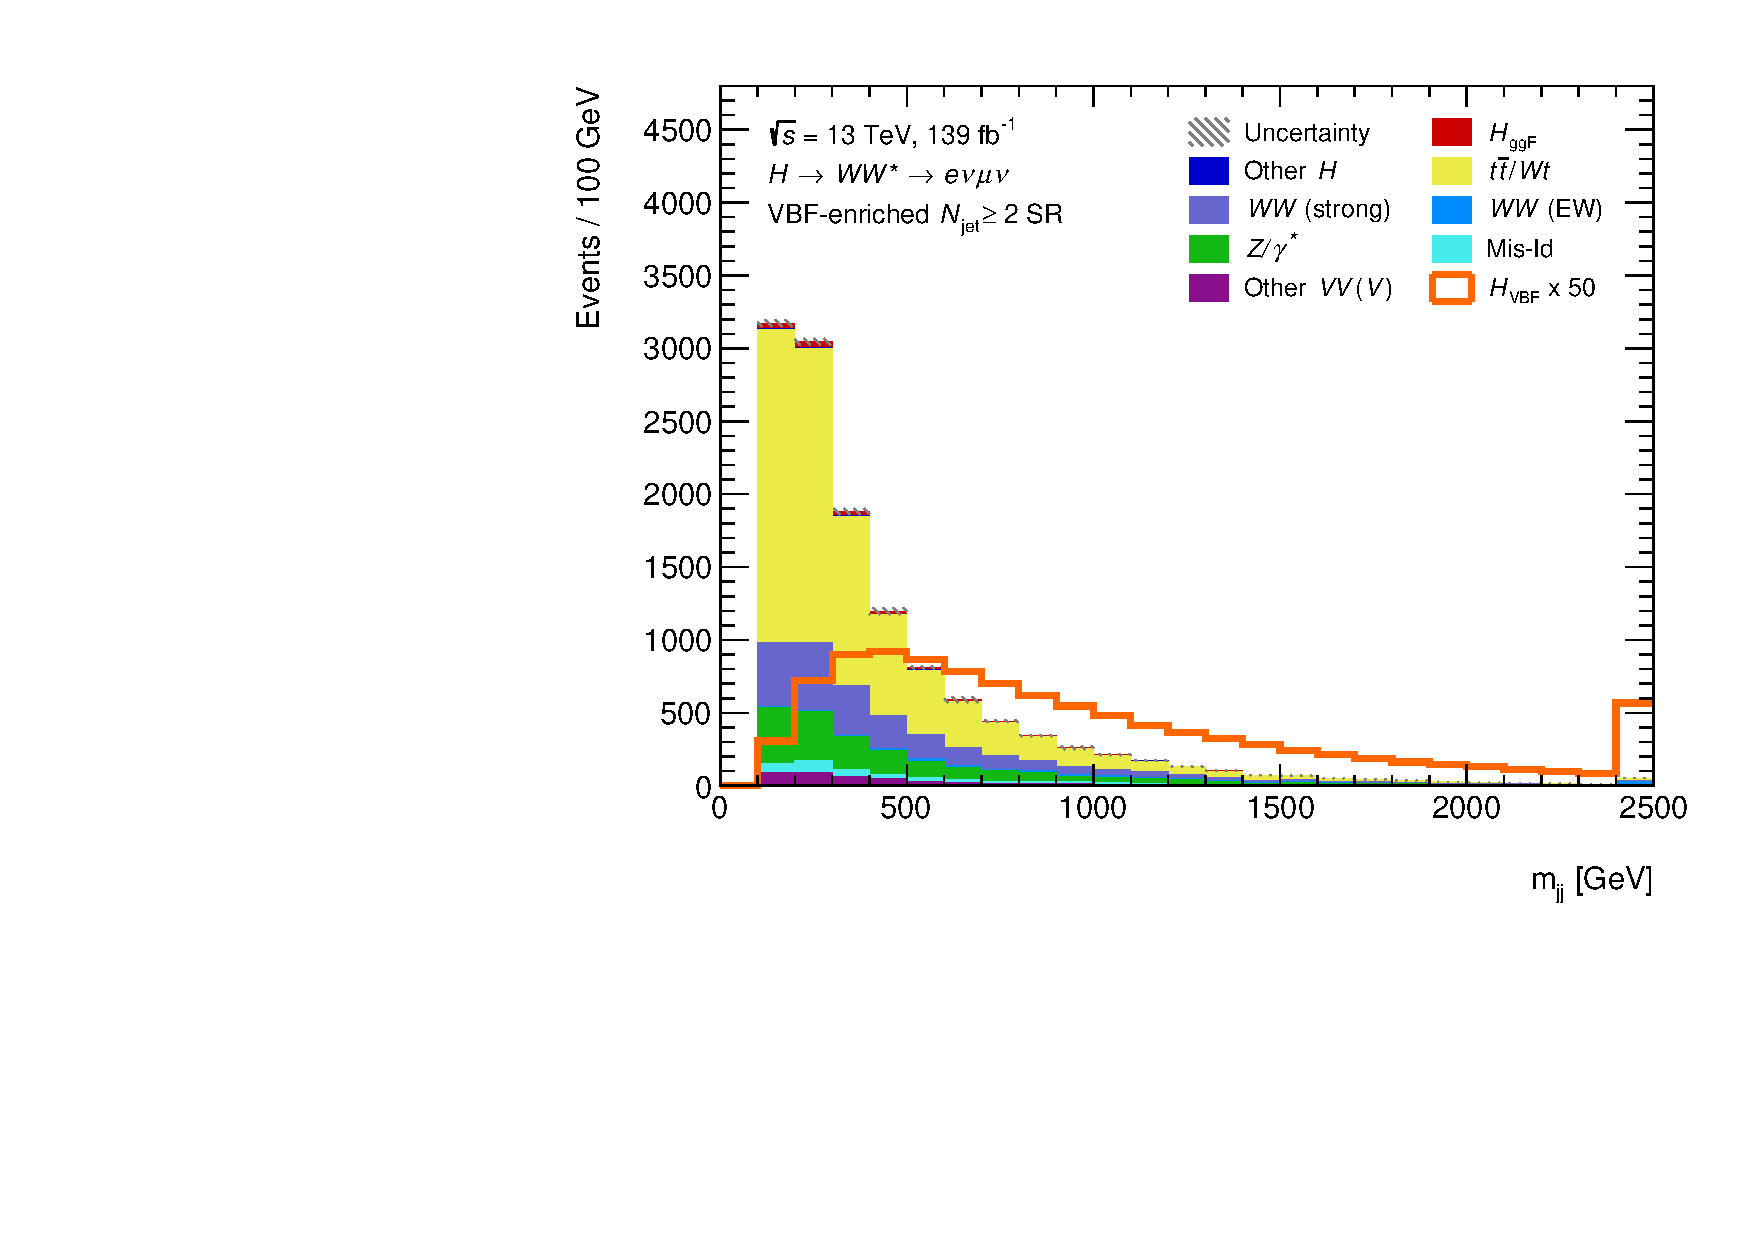
\includegraphics[width=0.32\textwidth]{figures/hww/dnn/blinded/run2-emme-CutVBF_SR-Mjj-lin.pdf} \hfill
        \label{fig:dnn-inputs-post-fit-1}
    } 
    \subfloat[$\dyjj$]{
        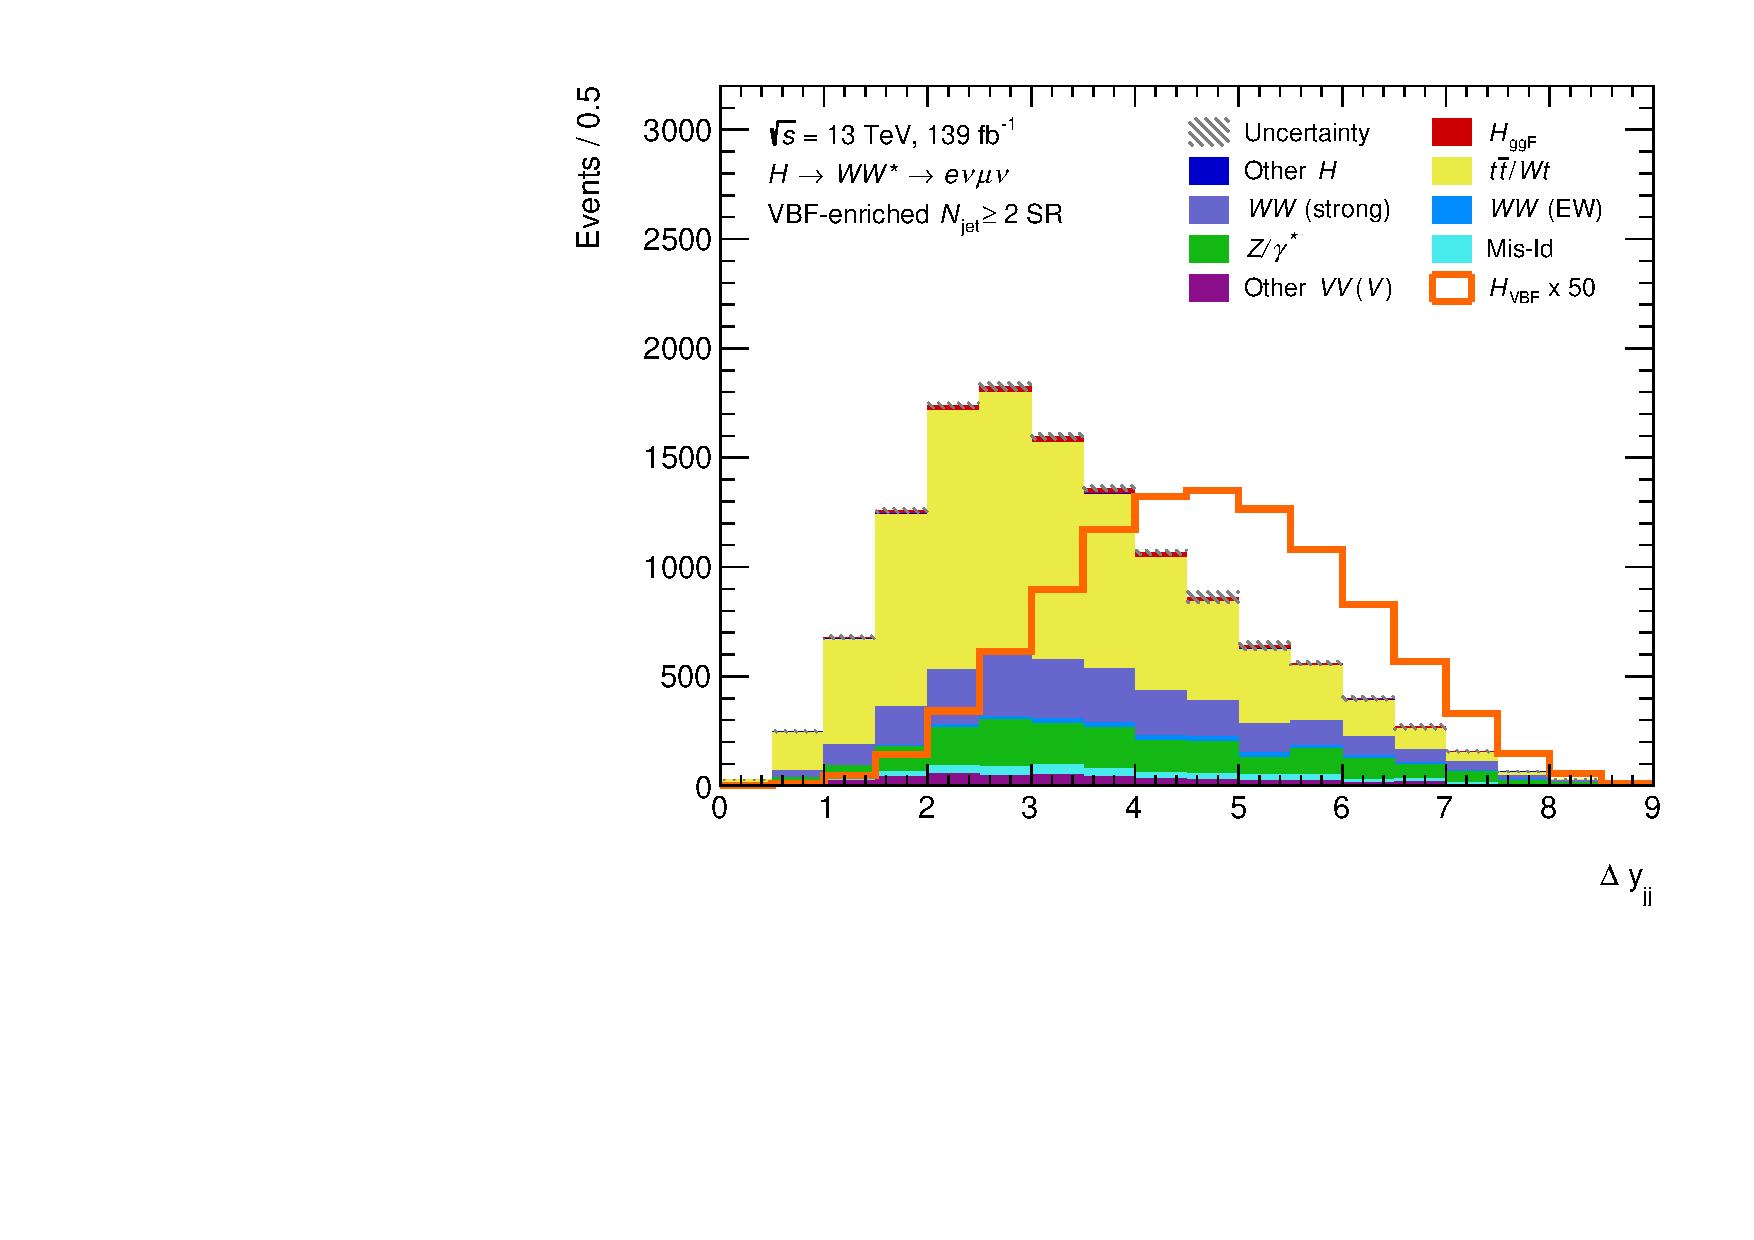
\includegraphics[width=0.32\textwidth]{figures/hww/dnn/blinded/run2-emme-CutVBF_SR-DYjj-lin.pdf} \hfill
        \label{fig:dnn-inputs-post-fit-2}
    } 
    \subfloat[$\lepetacent$]{
        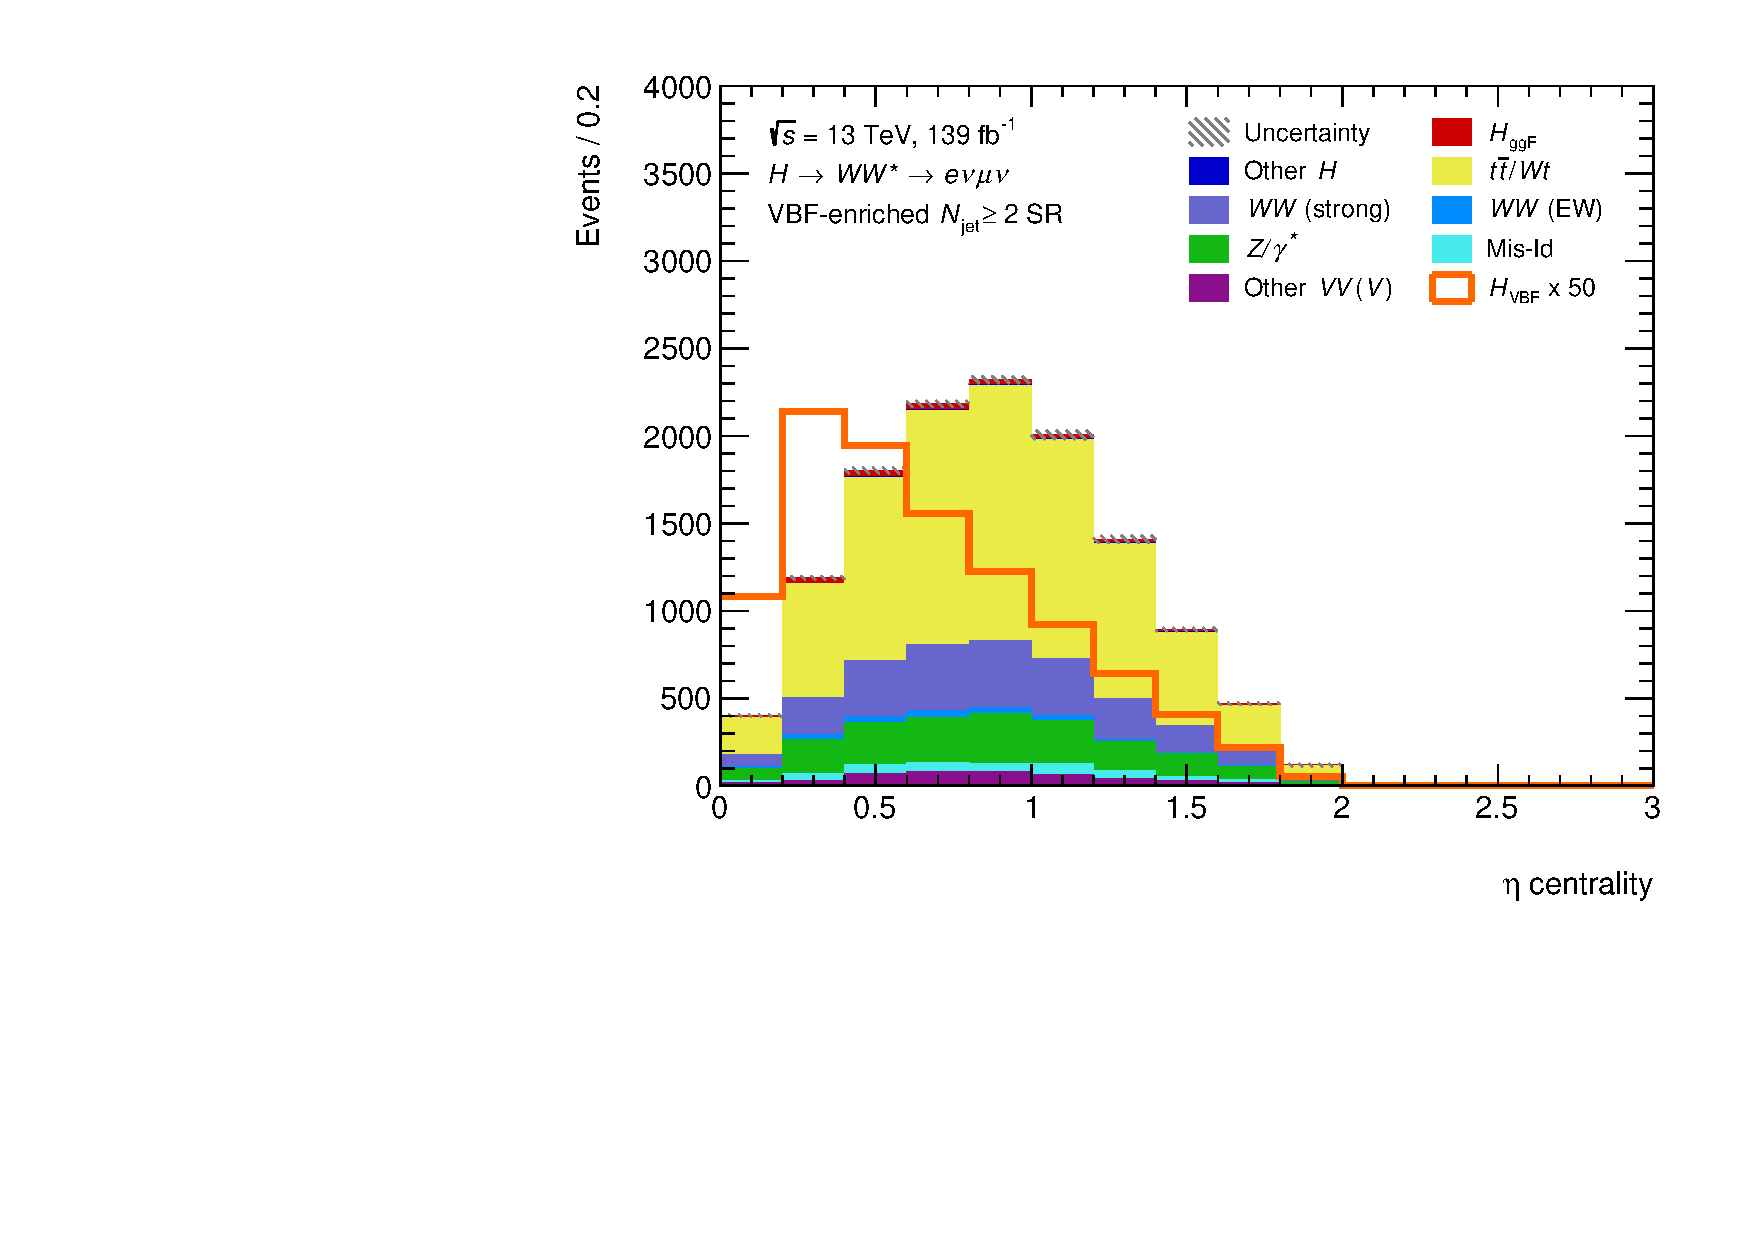
\includegraphics[width=0.32\textwidth]{figures/hww/dnn/blinded/run2-emme-CutVBF_SR-contOLV-lin.pdf} \hfill
        \label{fig:dnn-inputs-post-fit-3}
    } \\
    \subfloat[$\mlonejtwo$]{
        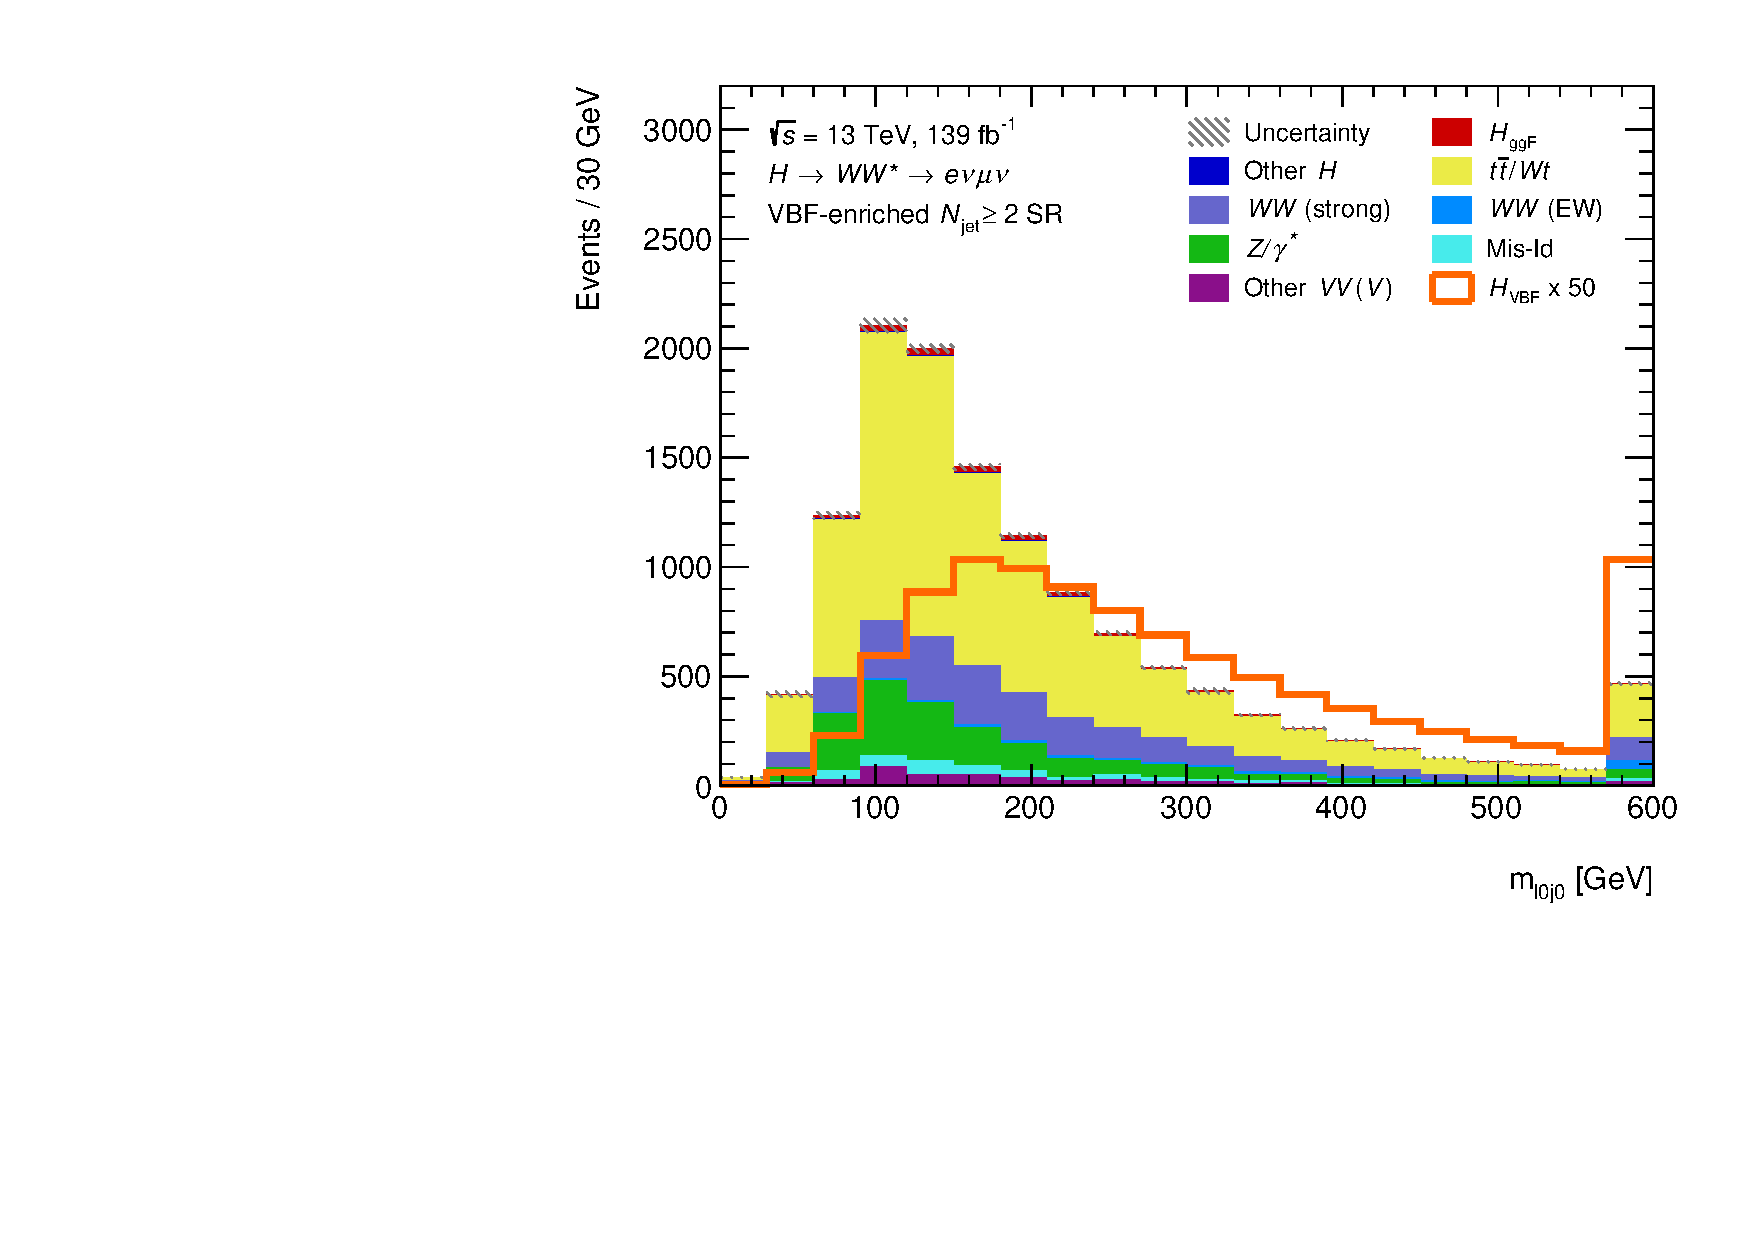
\includegraphics[width=0.32\textwidth]{figures/hww/dnn/blinded/run2-emme-CutVBF_SR-Ml0j0-lin.pdf} \hfill
        \label{fig:dnn-inputs-post-fit-4}
    } 
    \subfloat[$\mltwojone$]{
        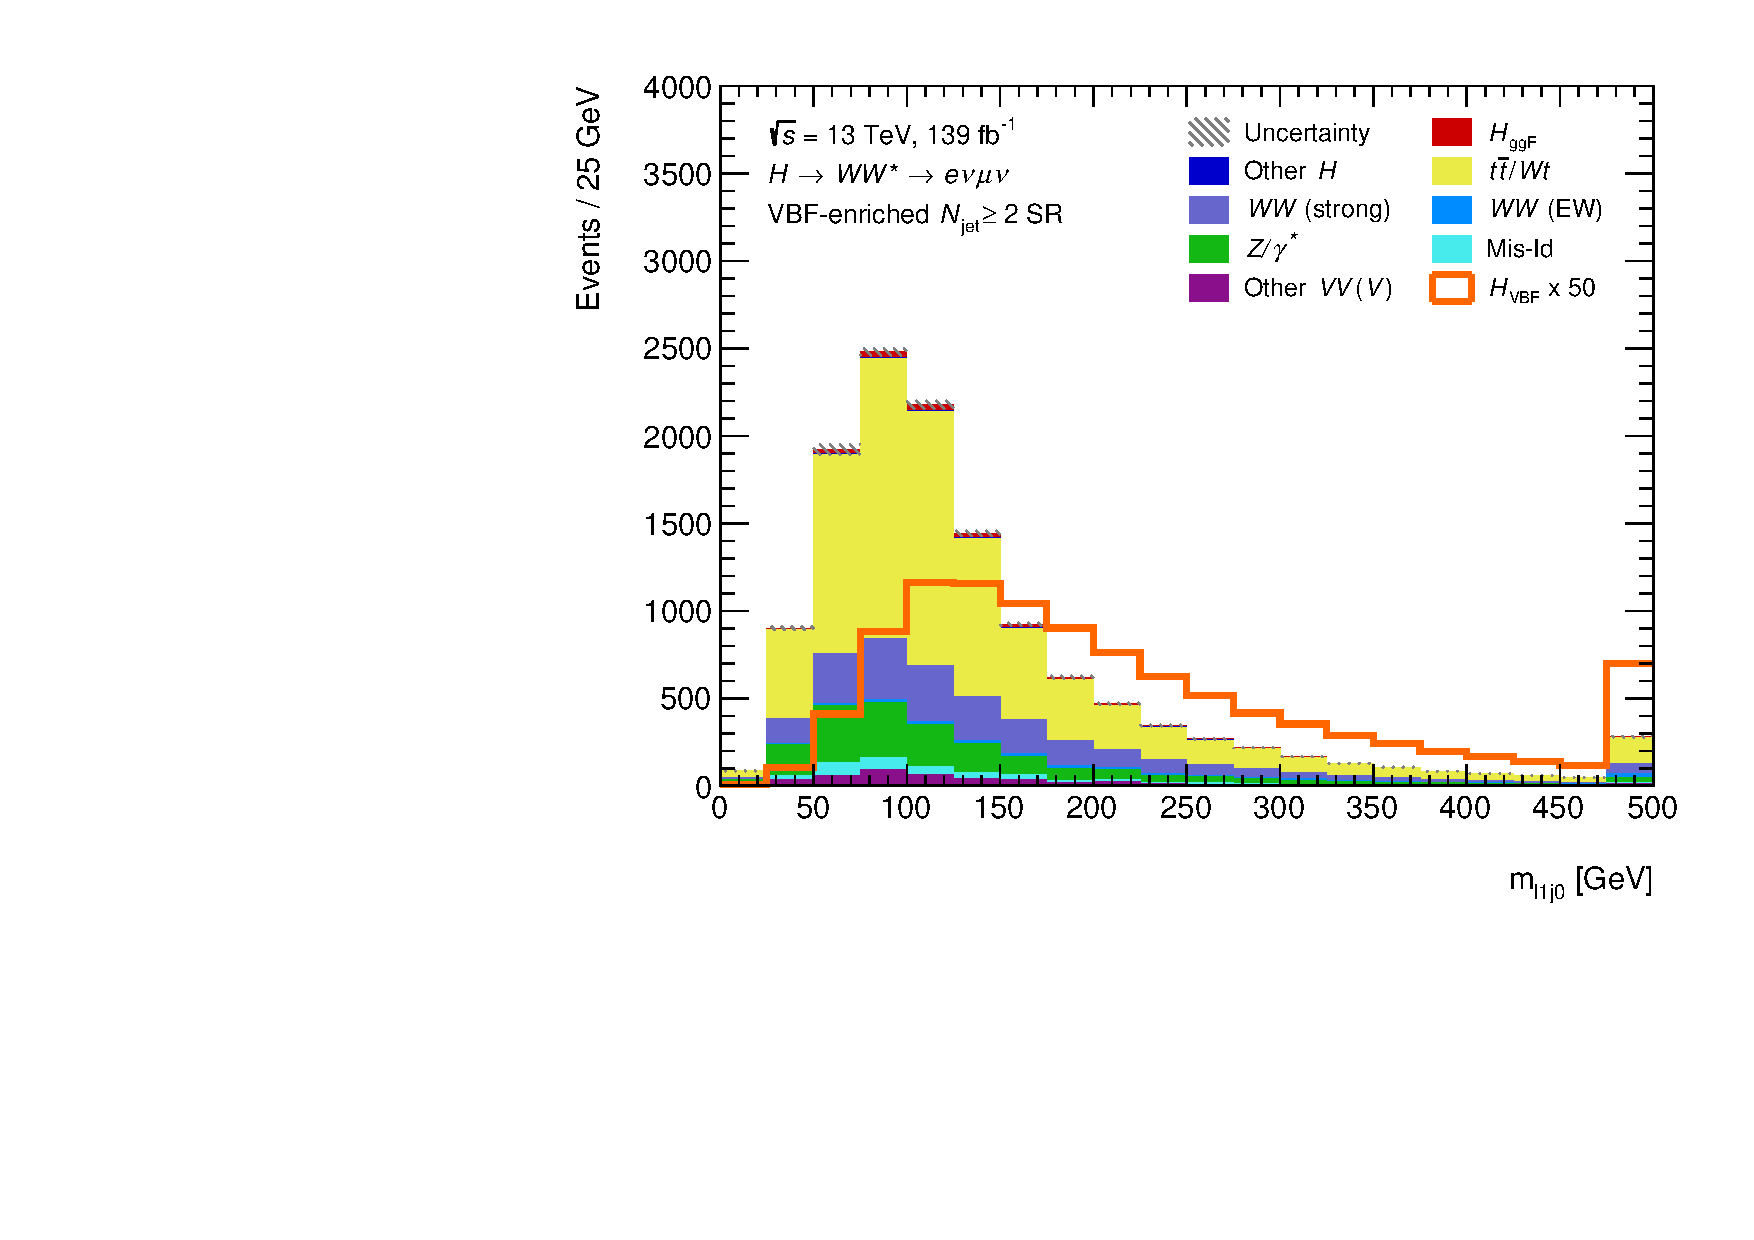
\includegraphics[width=0.32\textwidth]{figures/hww/dnn/blinded/run2-emme-CutVBF_SR-Ml1j0-lin.pdf} \hfill
        \label{fig:dnn-inputs-post-fit-5}
    } 
    \subfloat[$\mlonejtwo$]{
        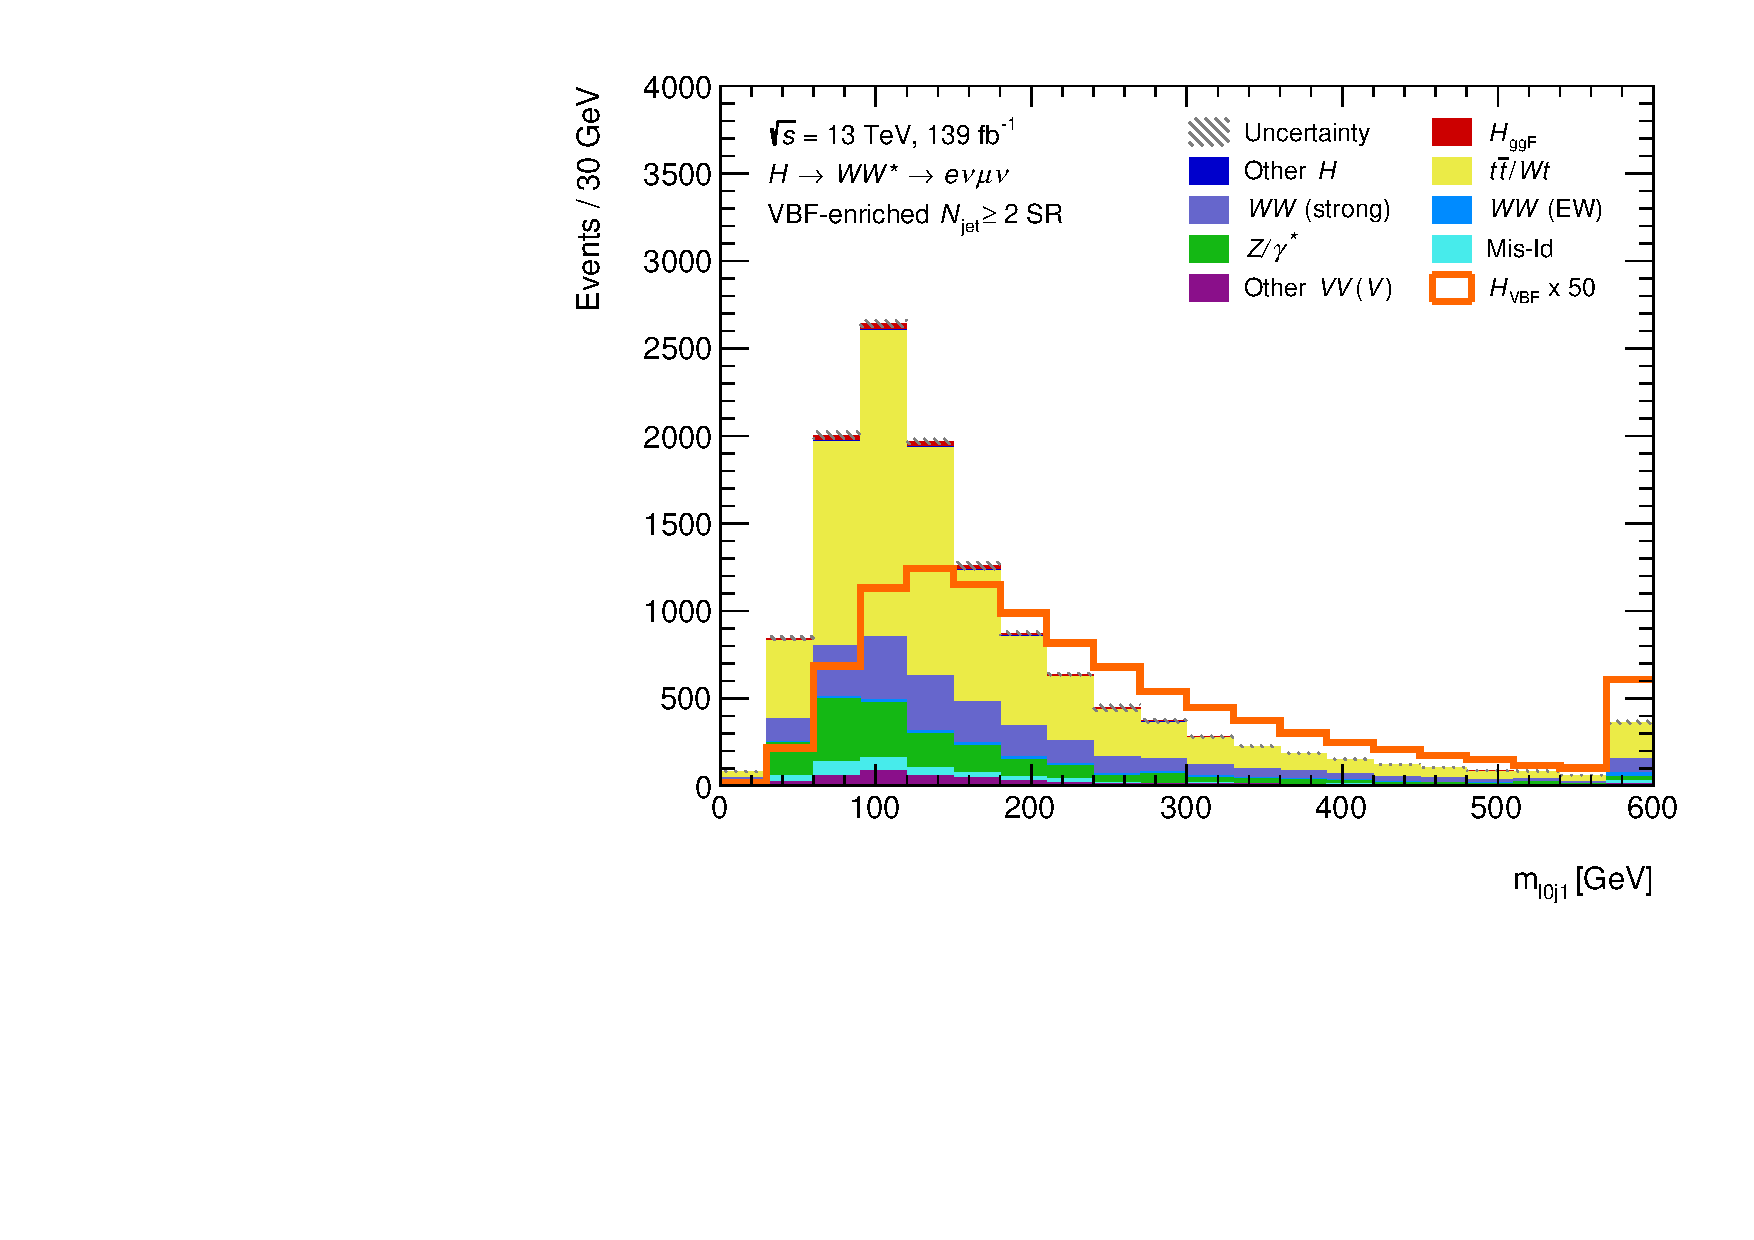
\includegraphics[width=0.32\textwidth]{figures/hww/dnn/blinded/run2-emme-CutVBF_SR-Ml0j1-lin.pdf} \hfill
        \label{fig:dnn-inputs-post-fit-6}
    } \\
    \subfloat[$\mltwojtwo$]{
        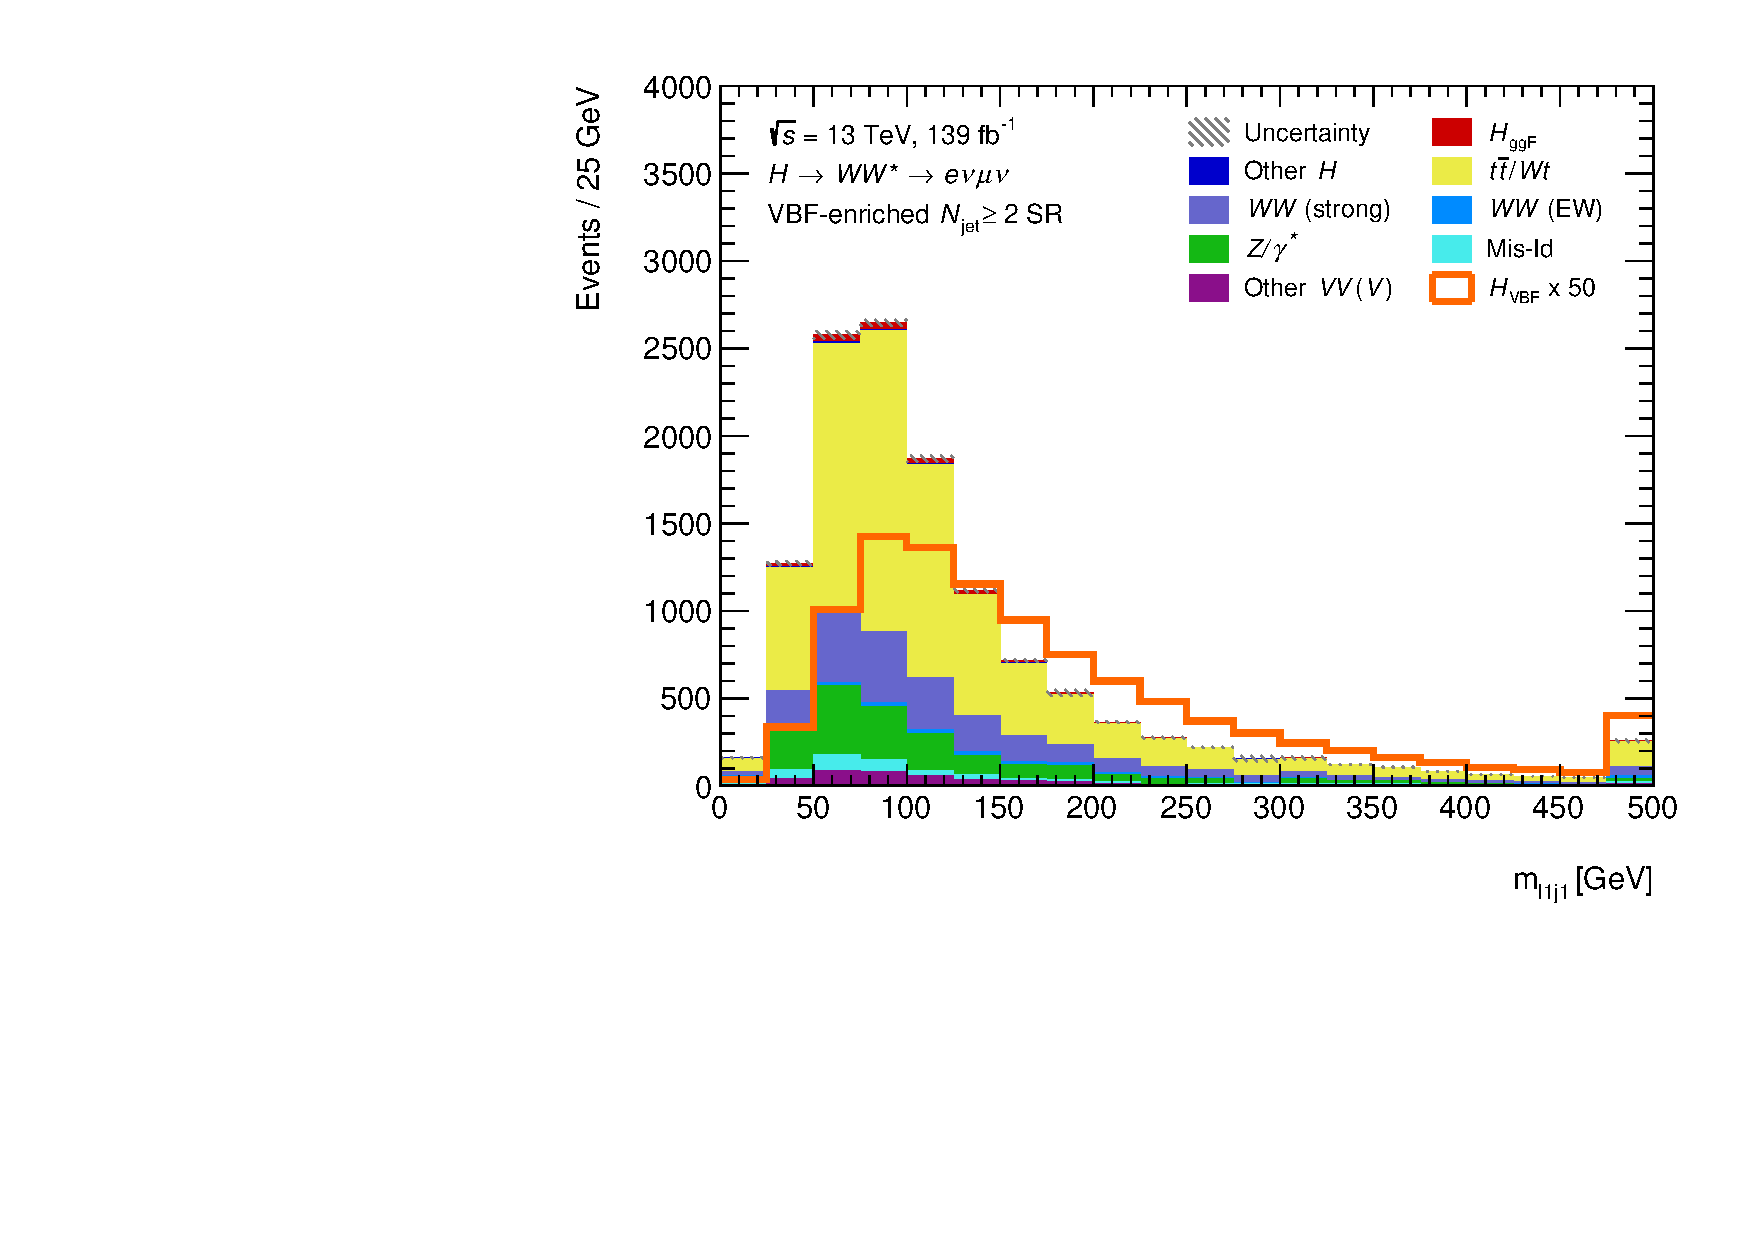
\includegraphics[width=0.32\textwidth]{figures/hww/dnn/blinded/run2-emme-CutVBF_SR-Ml1j1-lin.pdf} \hfill
        \label{fig:dnn-inputs-post-fit-7}
    } 
    \subfloat[$\pTjone$]{
        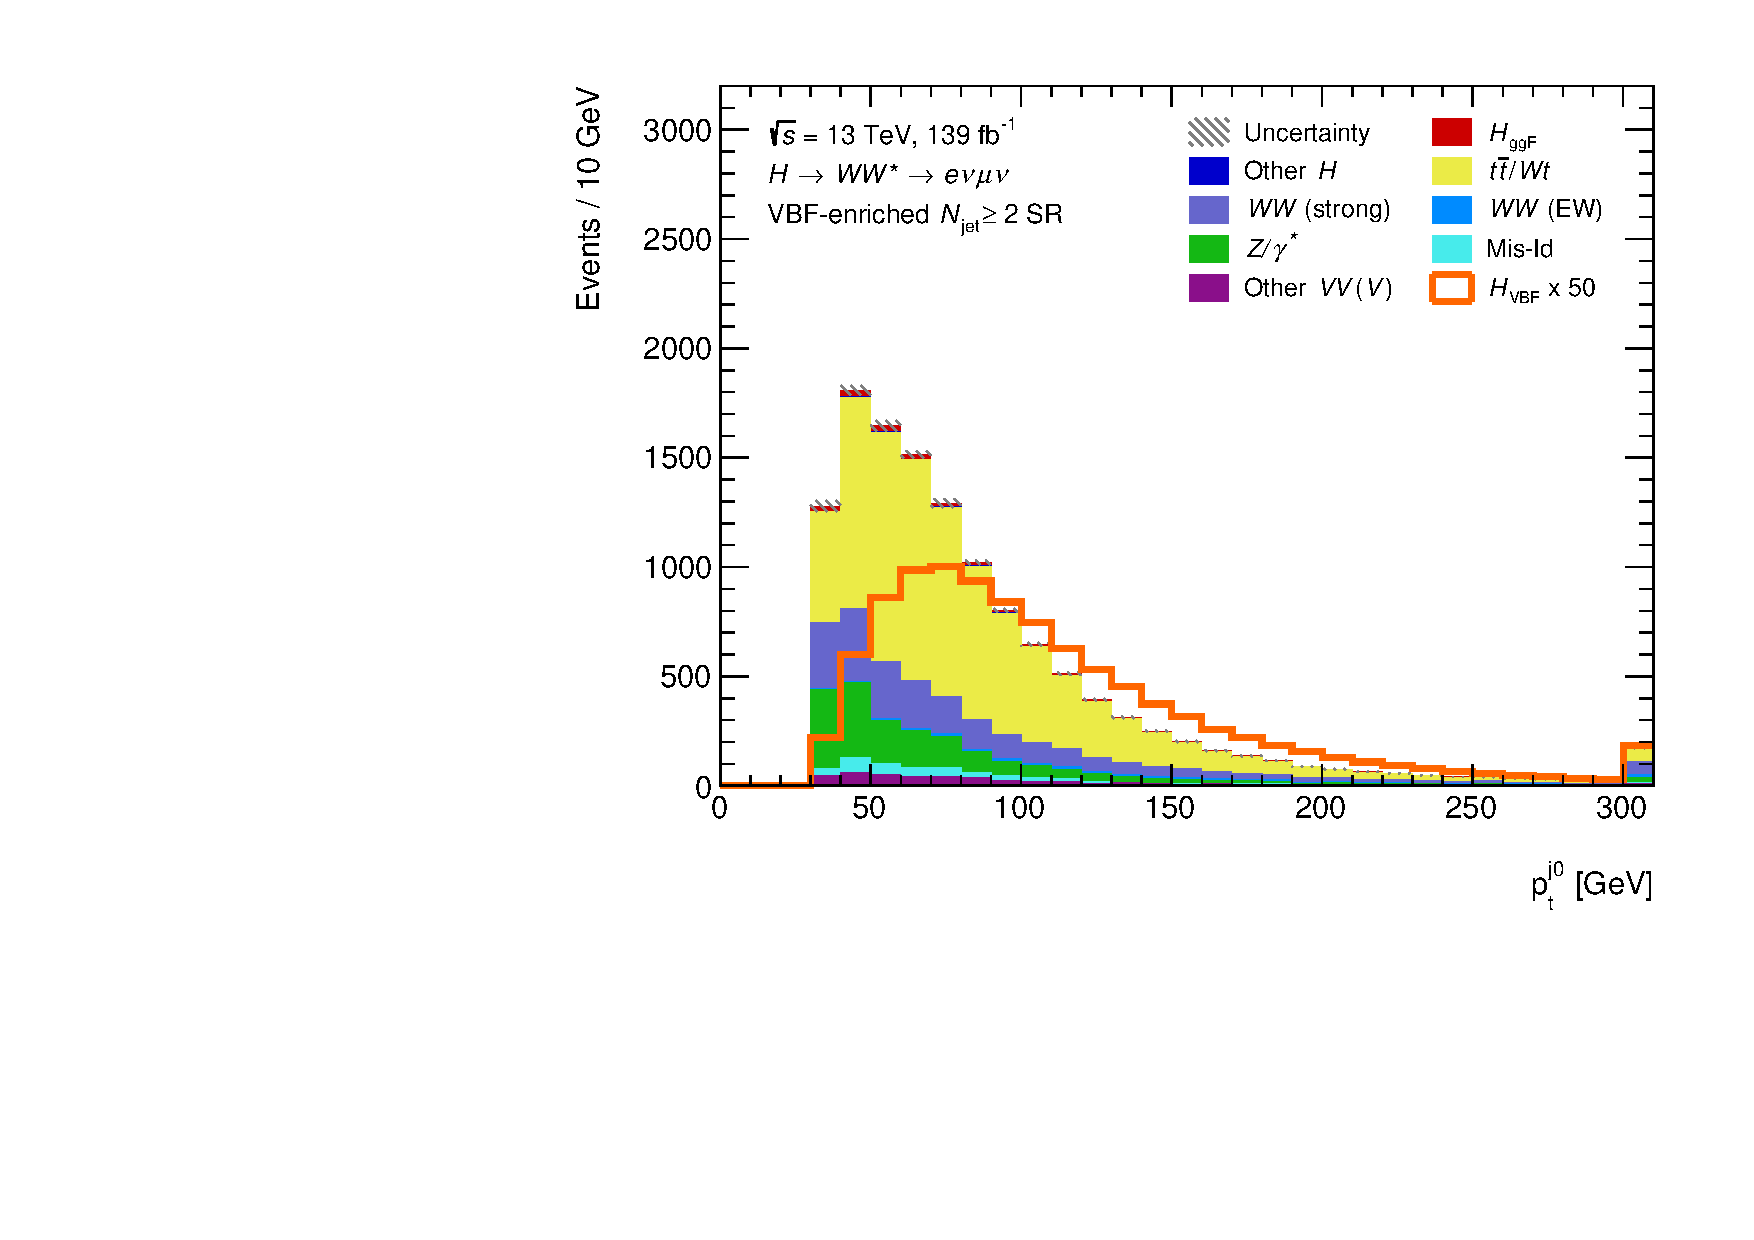
\includegraphics[width=0.32\textwidth]{figures/hww/dnn/blinded/run2-emme-CutVBF_SR-leadJetPt-lin.pdf} \hfill
        \label{fig:dnn-inputs-post-fit-8}
    } 
    \subfloat[$\pTjtwo$]{
        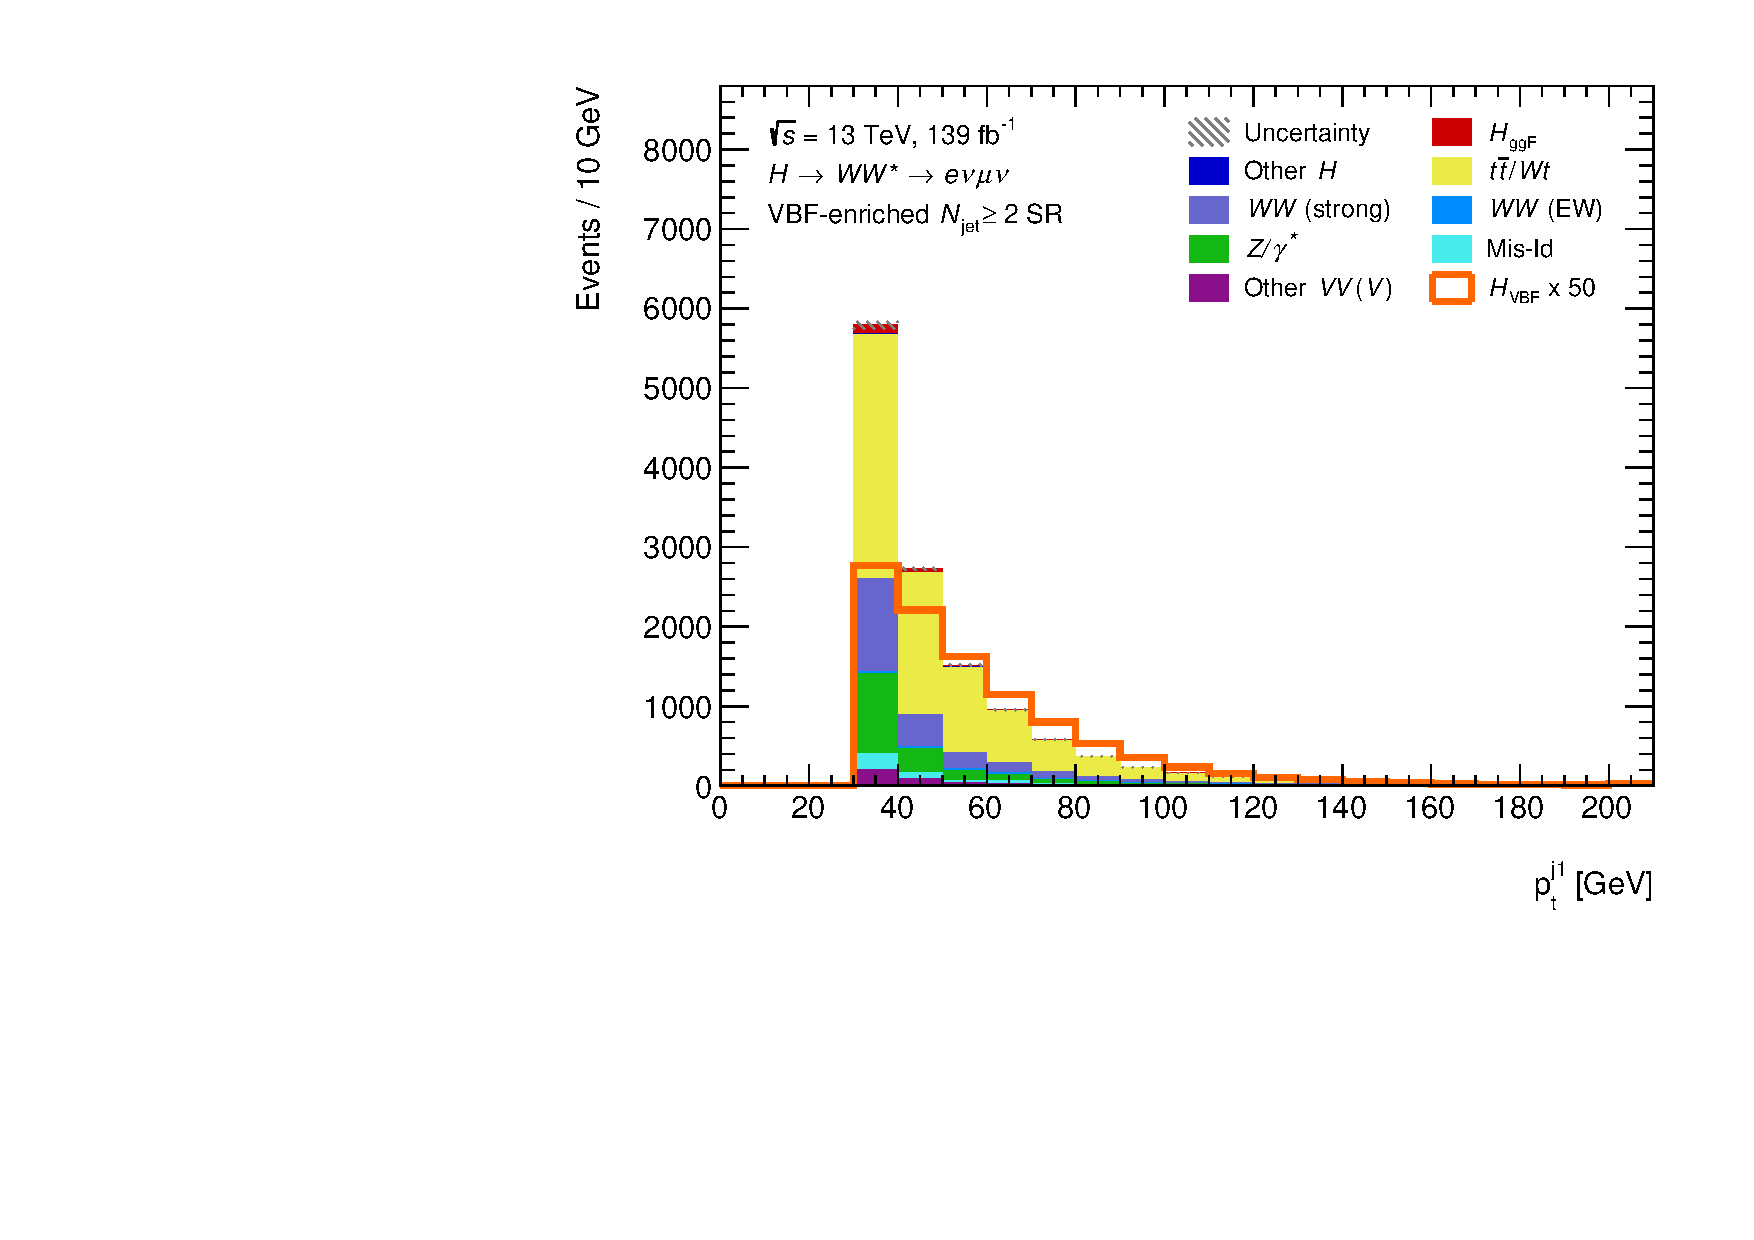
\includegraphics[width=0.32\textwidth]{figures/hww/dnn/blinded/run2-emme-CutVBF_SR-subleadJetPt-lin.pdf} \hfill
        \label{fig:dnn-inputs-post-fit-9}
    } \\
    \subfloat[$\pTjthree$]{
        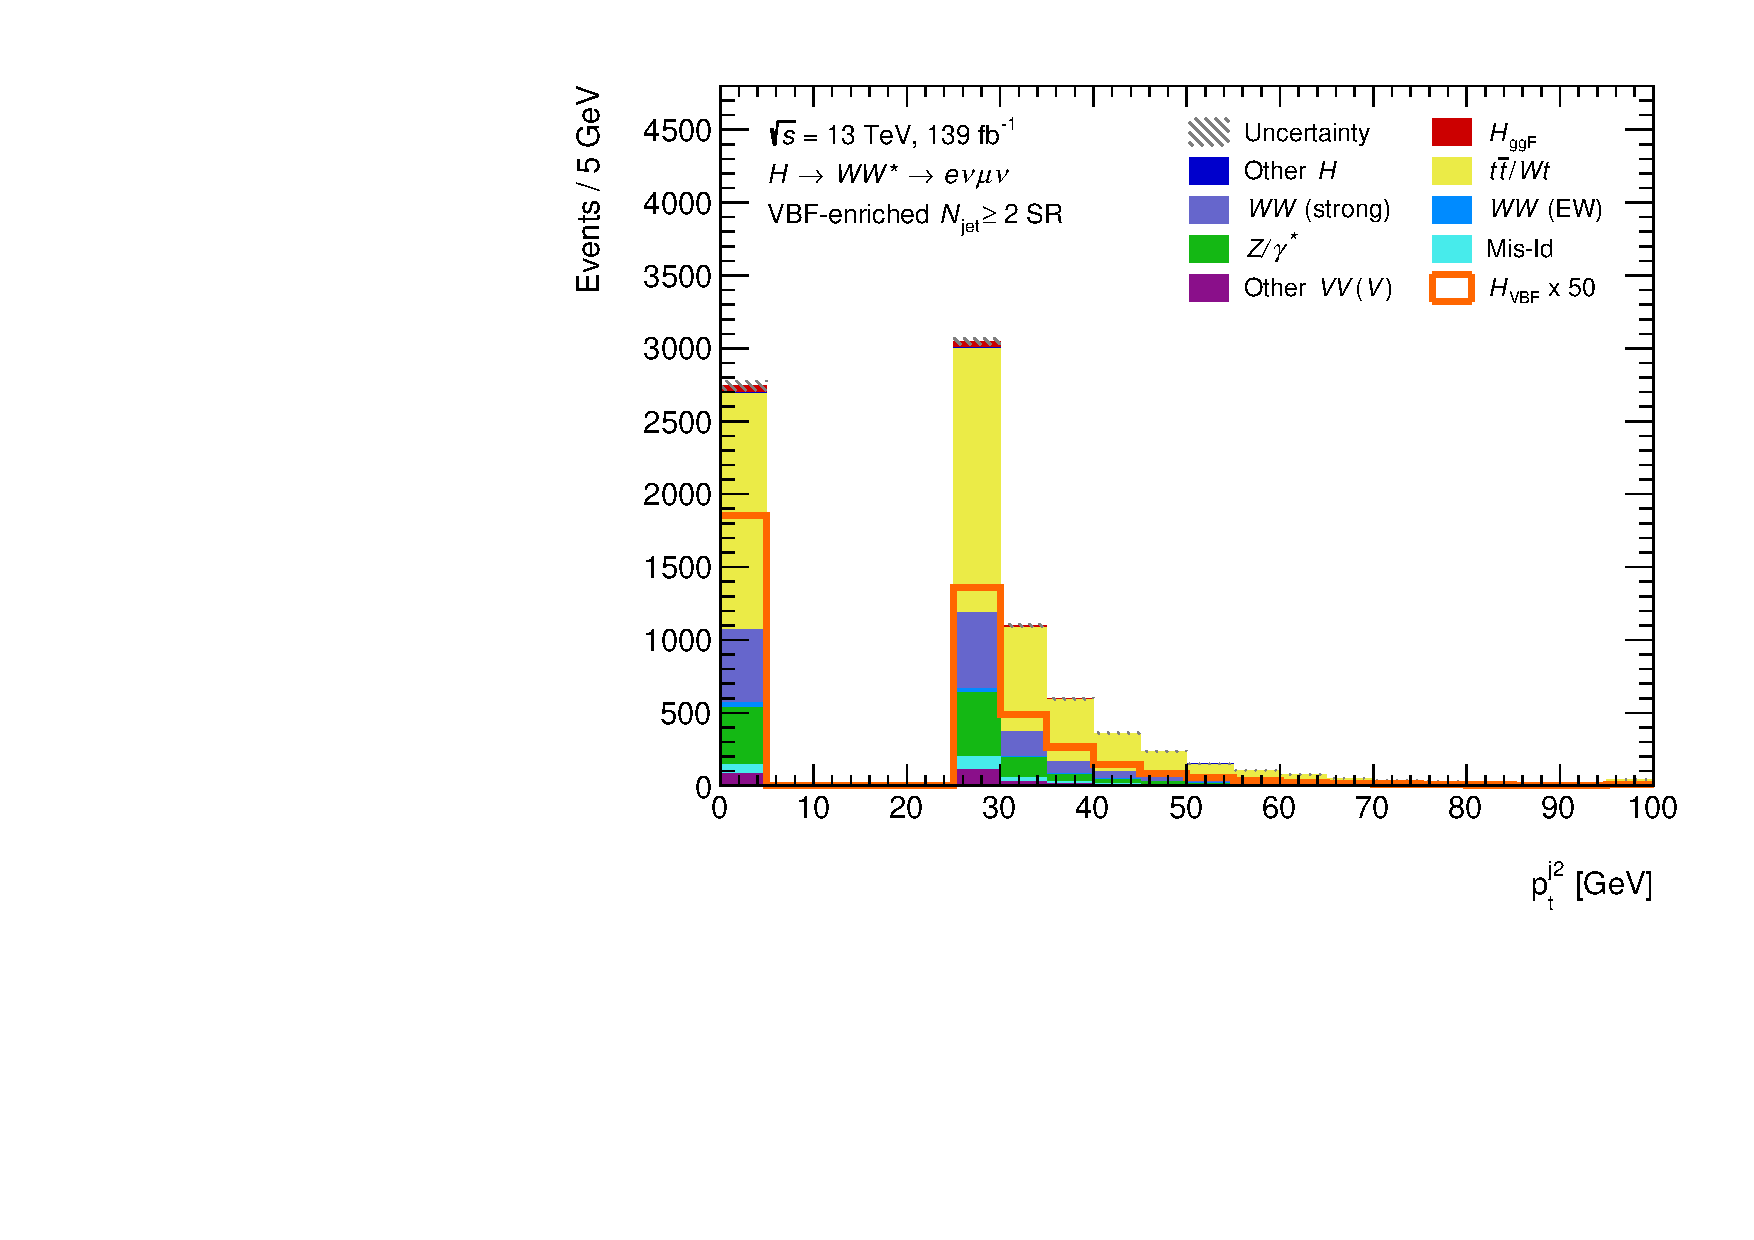
\includegraphics[width=0.32\textwidth]{figures/hww/dnn/blinded/run2-emme-CutVBF_SR-thirdJetPt-lin.pdf} \hfill
        \label{fig:dnn-inputs-post-fit-10}
    } 
    {\caption{Distributions of $\dphill$, $\mll$, $\lepetacent$, \pTjone, \pTjtwo, \pTjthree in the VBF signal region.
        Each row corresponds to one variable with different selections made on the DNN output.
        \label{fig:dnn-inputs-post-fit1} }}
\end{figure}


% \begin{figure}[h]
%     \centering
%     {\caption{Distributions of $\mlonejone$, $\mltwojone$, $\mlonejtwo$, and $\mltwojtwo$ in the VBF signal region.
%             Each row shows one variable with different cuts on the DNN output distribution being applied in different columns.
%             \label{app:fig:dnn-inputs-vbf-top2} }}
% \end{figure}


\begin{figure}[h]
    \centering
    \subfloat[$\dphill$]{
        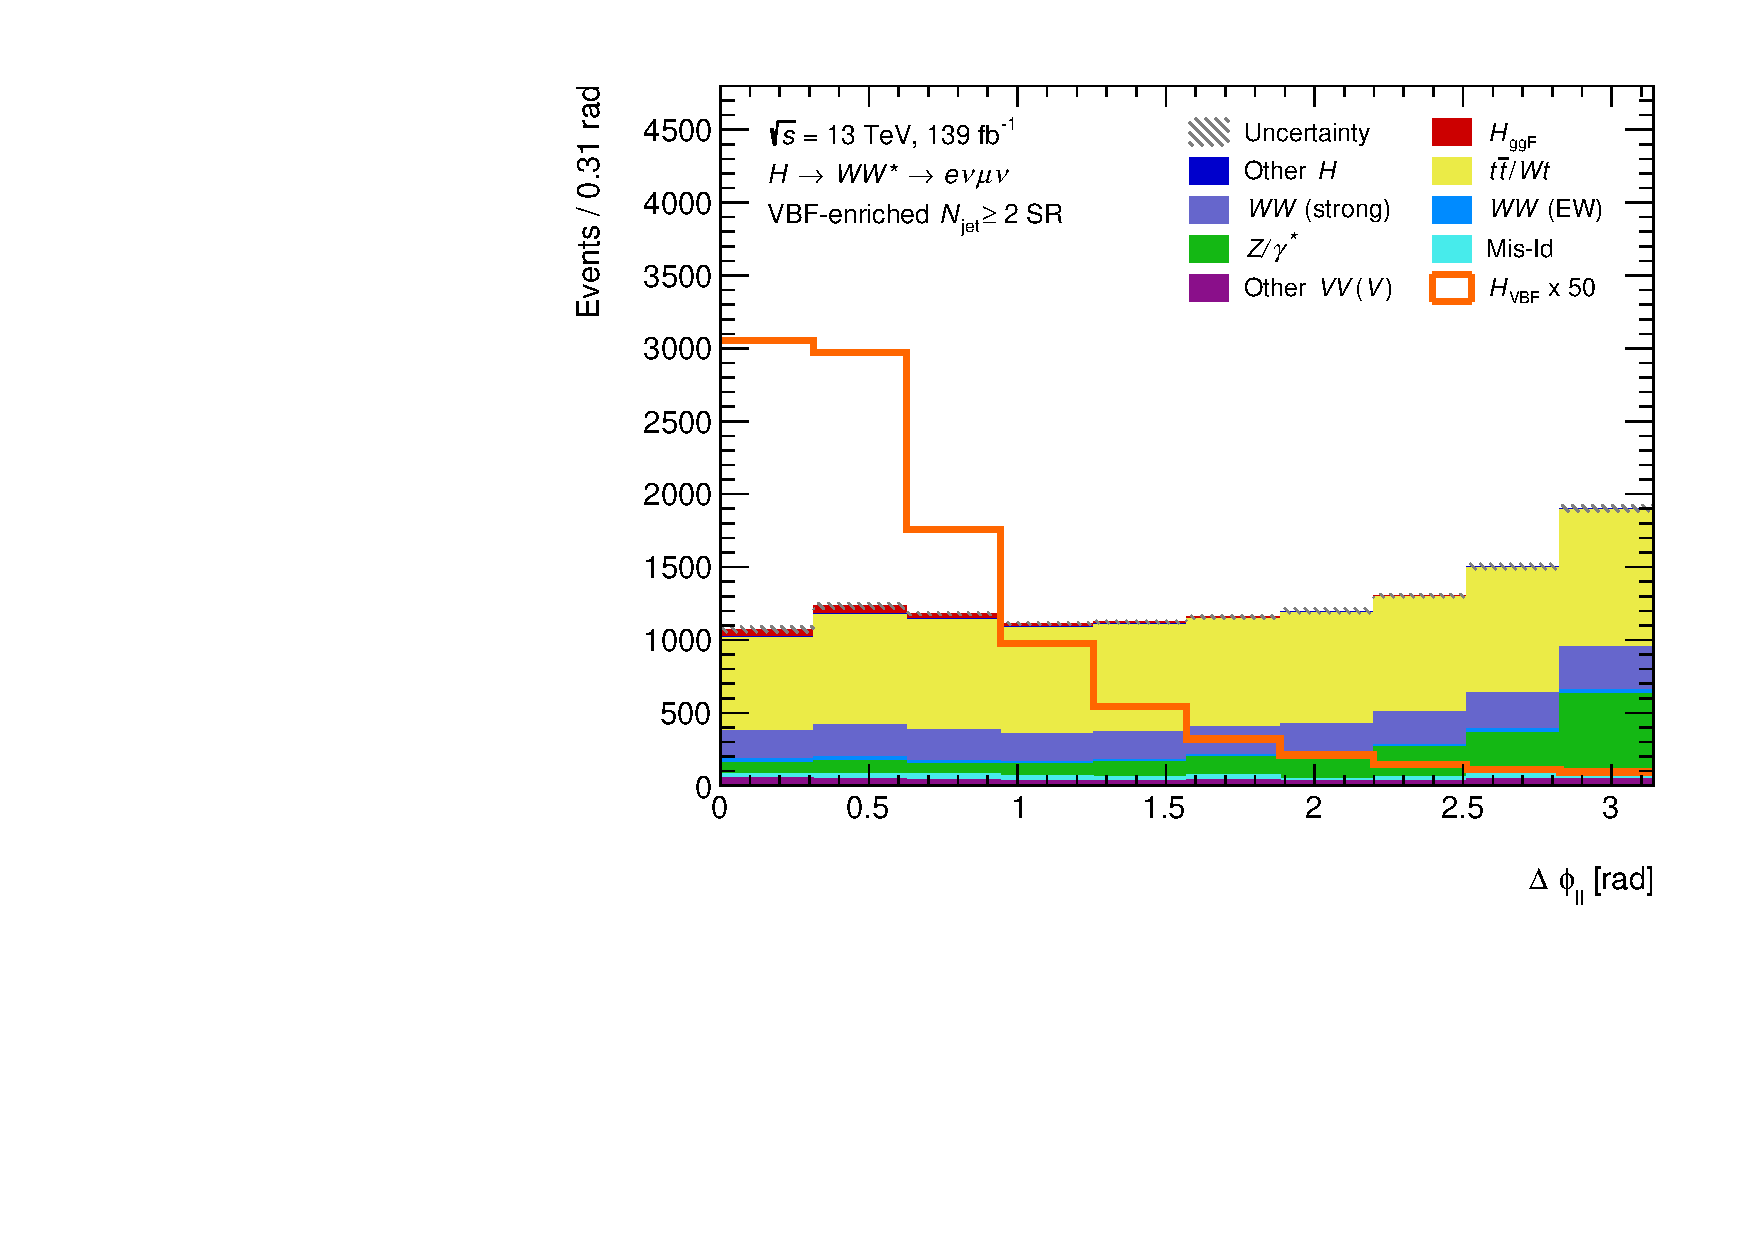
\includegraphics[width=0.32\textwidth]{figures/hww/dnn/blinded/run2-emme-CutVBF_SR-DPhill-lin.pdf} \hfill
        \label{fig:dnn-inputs-post-fit2-1}
    } 
    \subfloat[$\mll$]{
        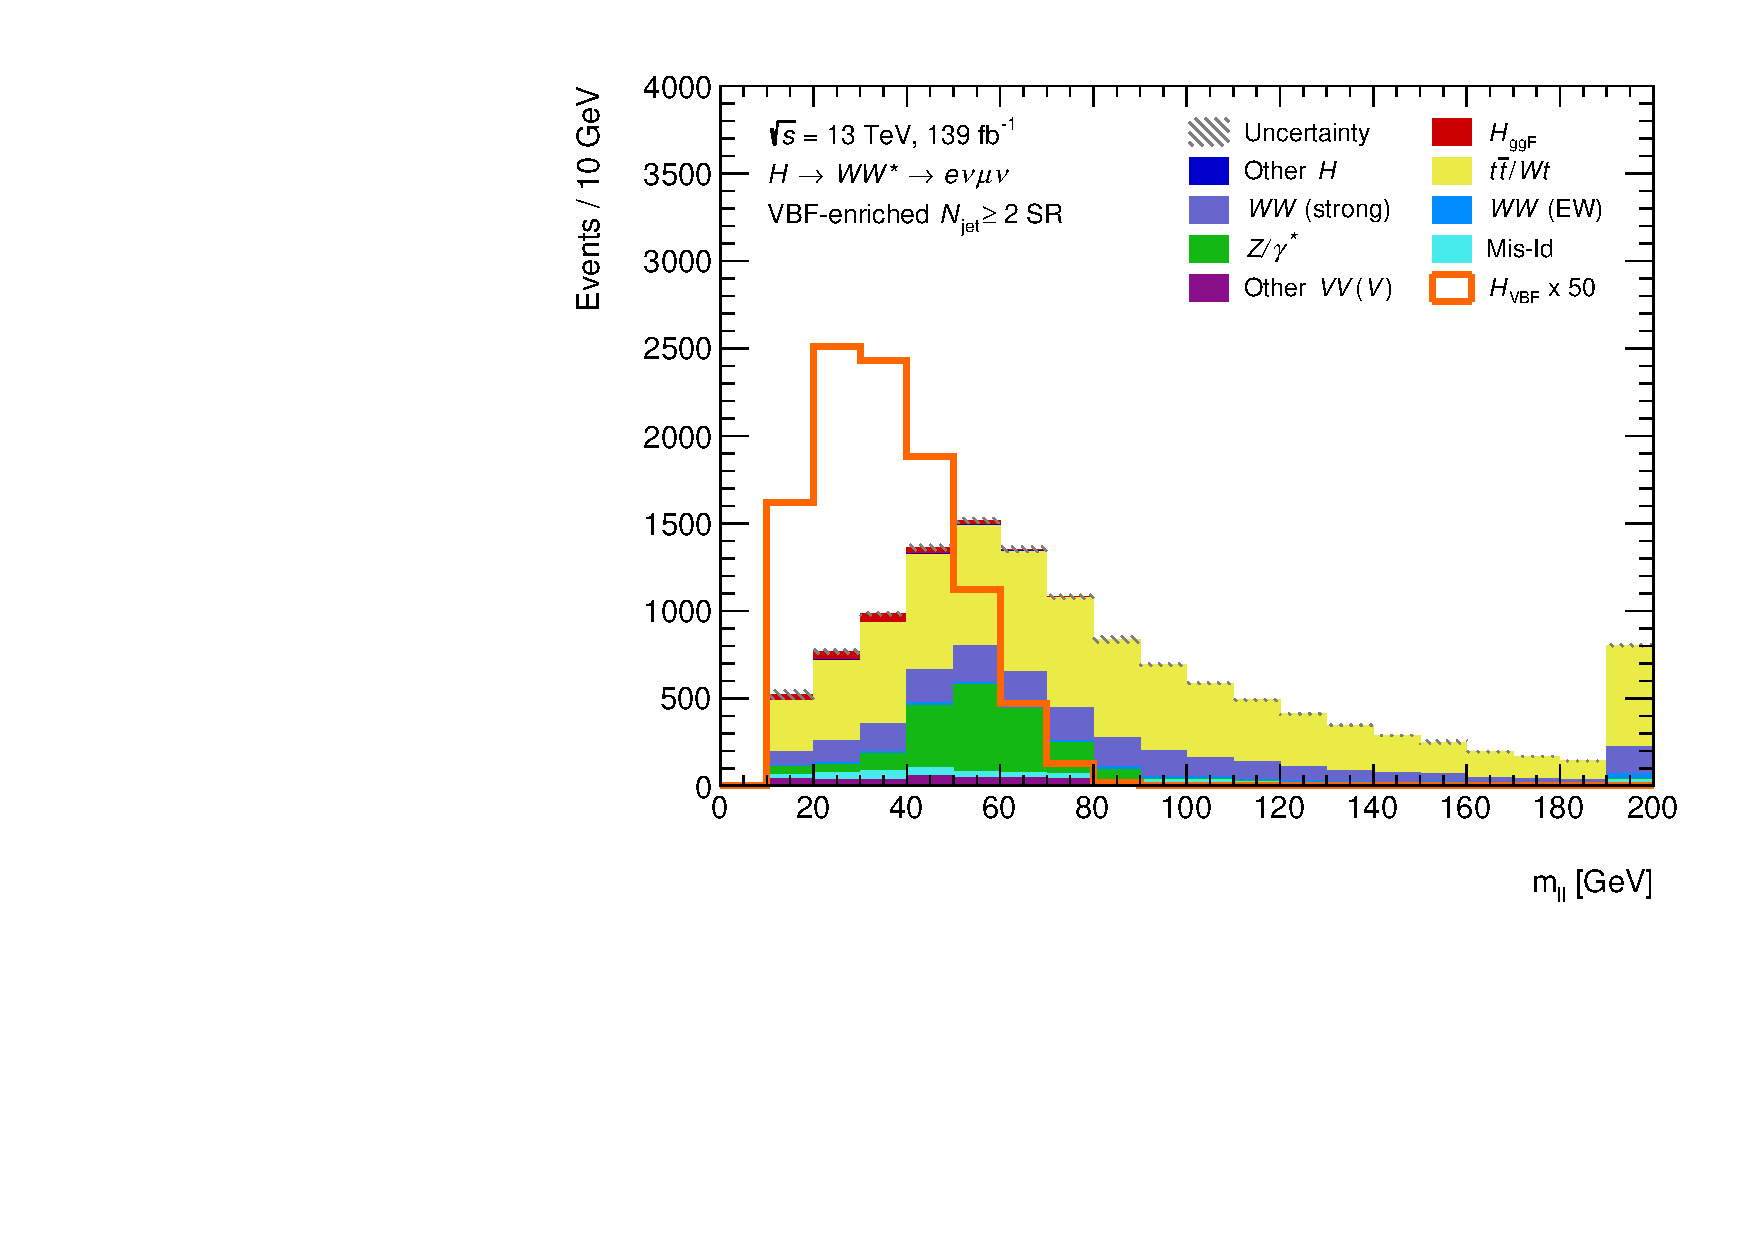
\includegraphics[width=0.32\textwidth]{figures/hww/dnn/blinded/run2-emme-CutVBF_SR-Mll-lin.pdf}
        \label{fig:dnn-inputs-post-fit2-2}
    } 
    \subfloat[$\mT$]{
        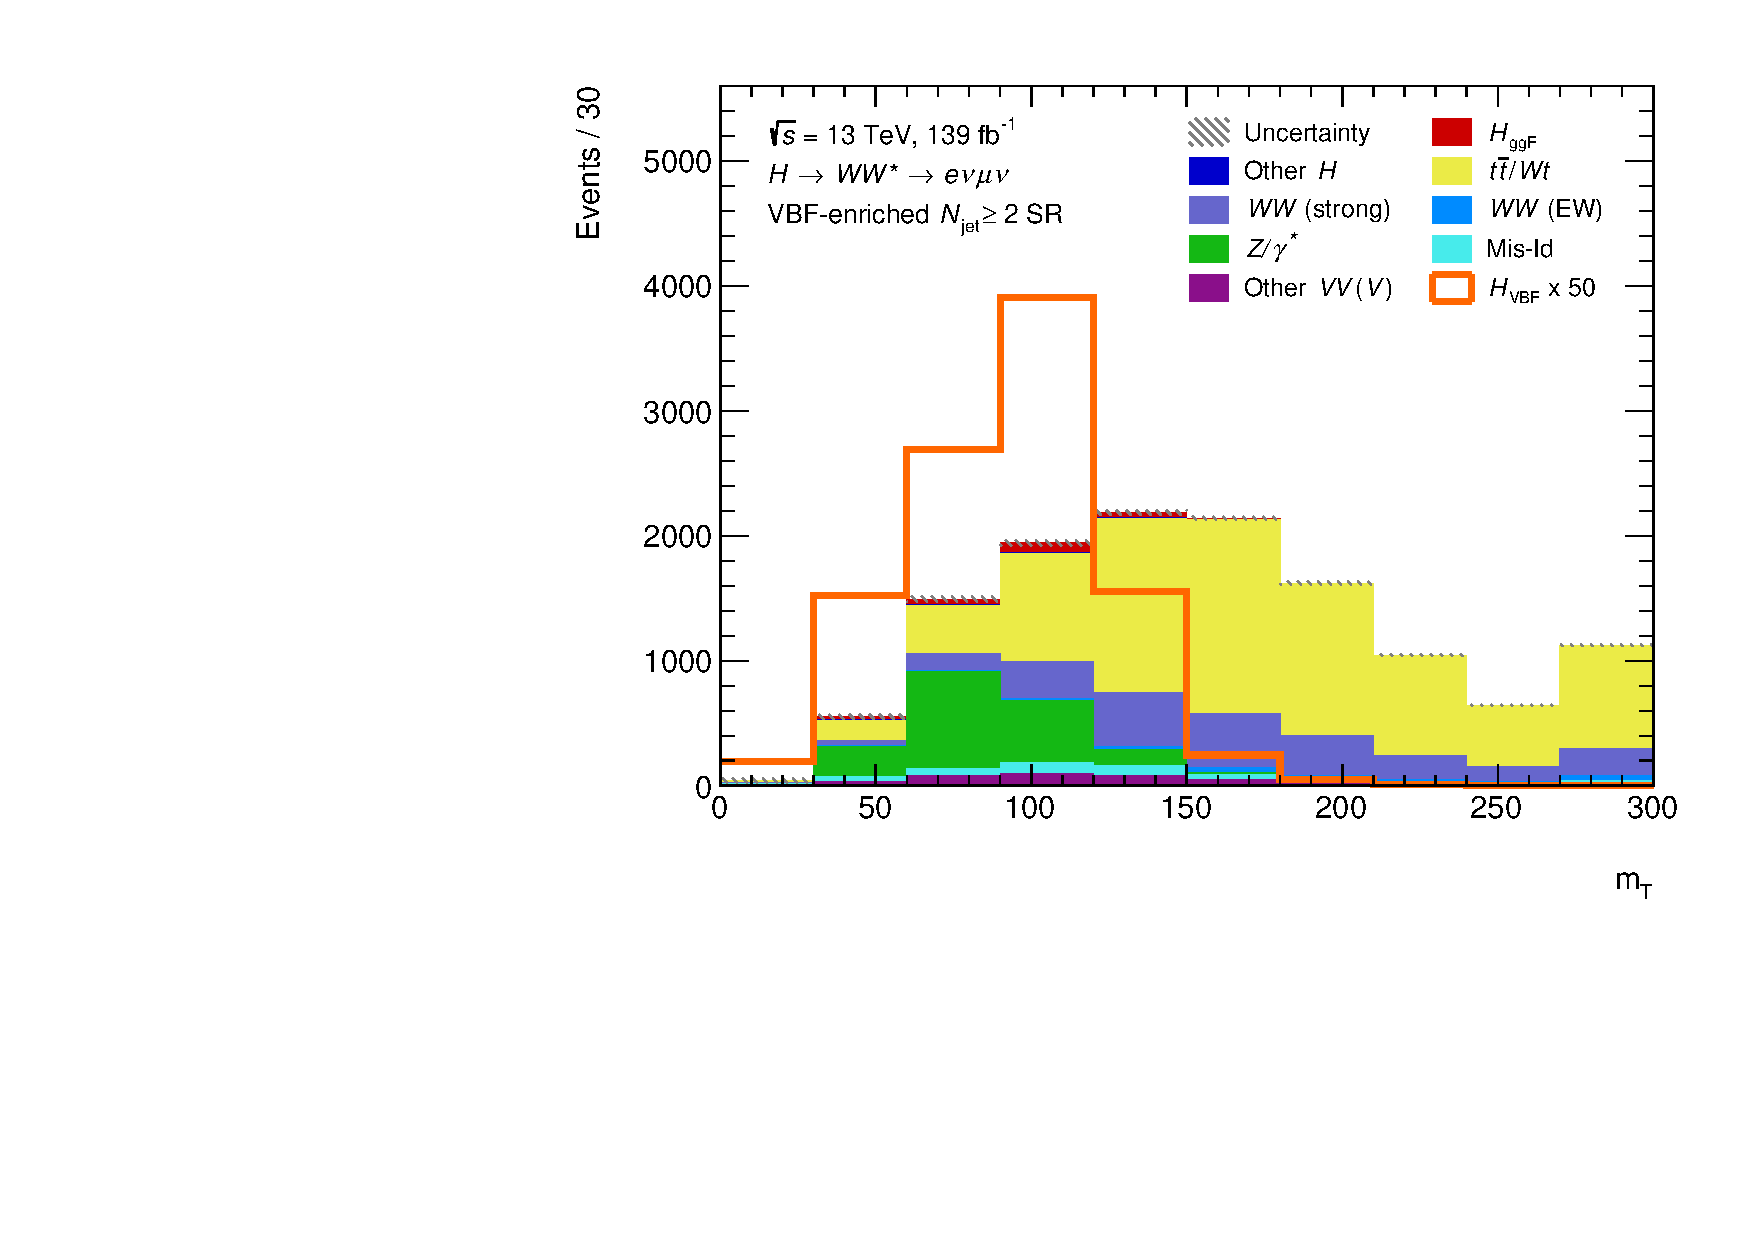
\includegraphics[width=0.32\textwidth]{figures/hww/dnn/blinded/run2-emme-CutVBF_SR-MT-lin.pdf} \hfill
        \label{fig:dnn-inputs-post-fit2-3}
    } \\
    \subfloat[$\pttot$]{
        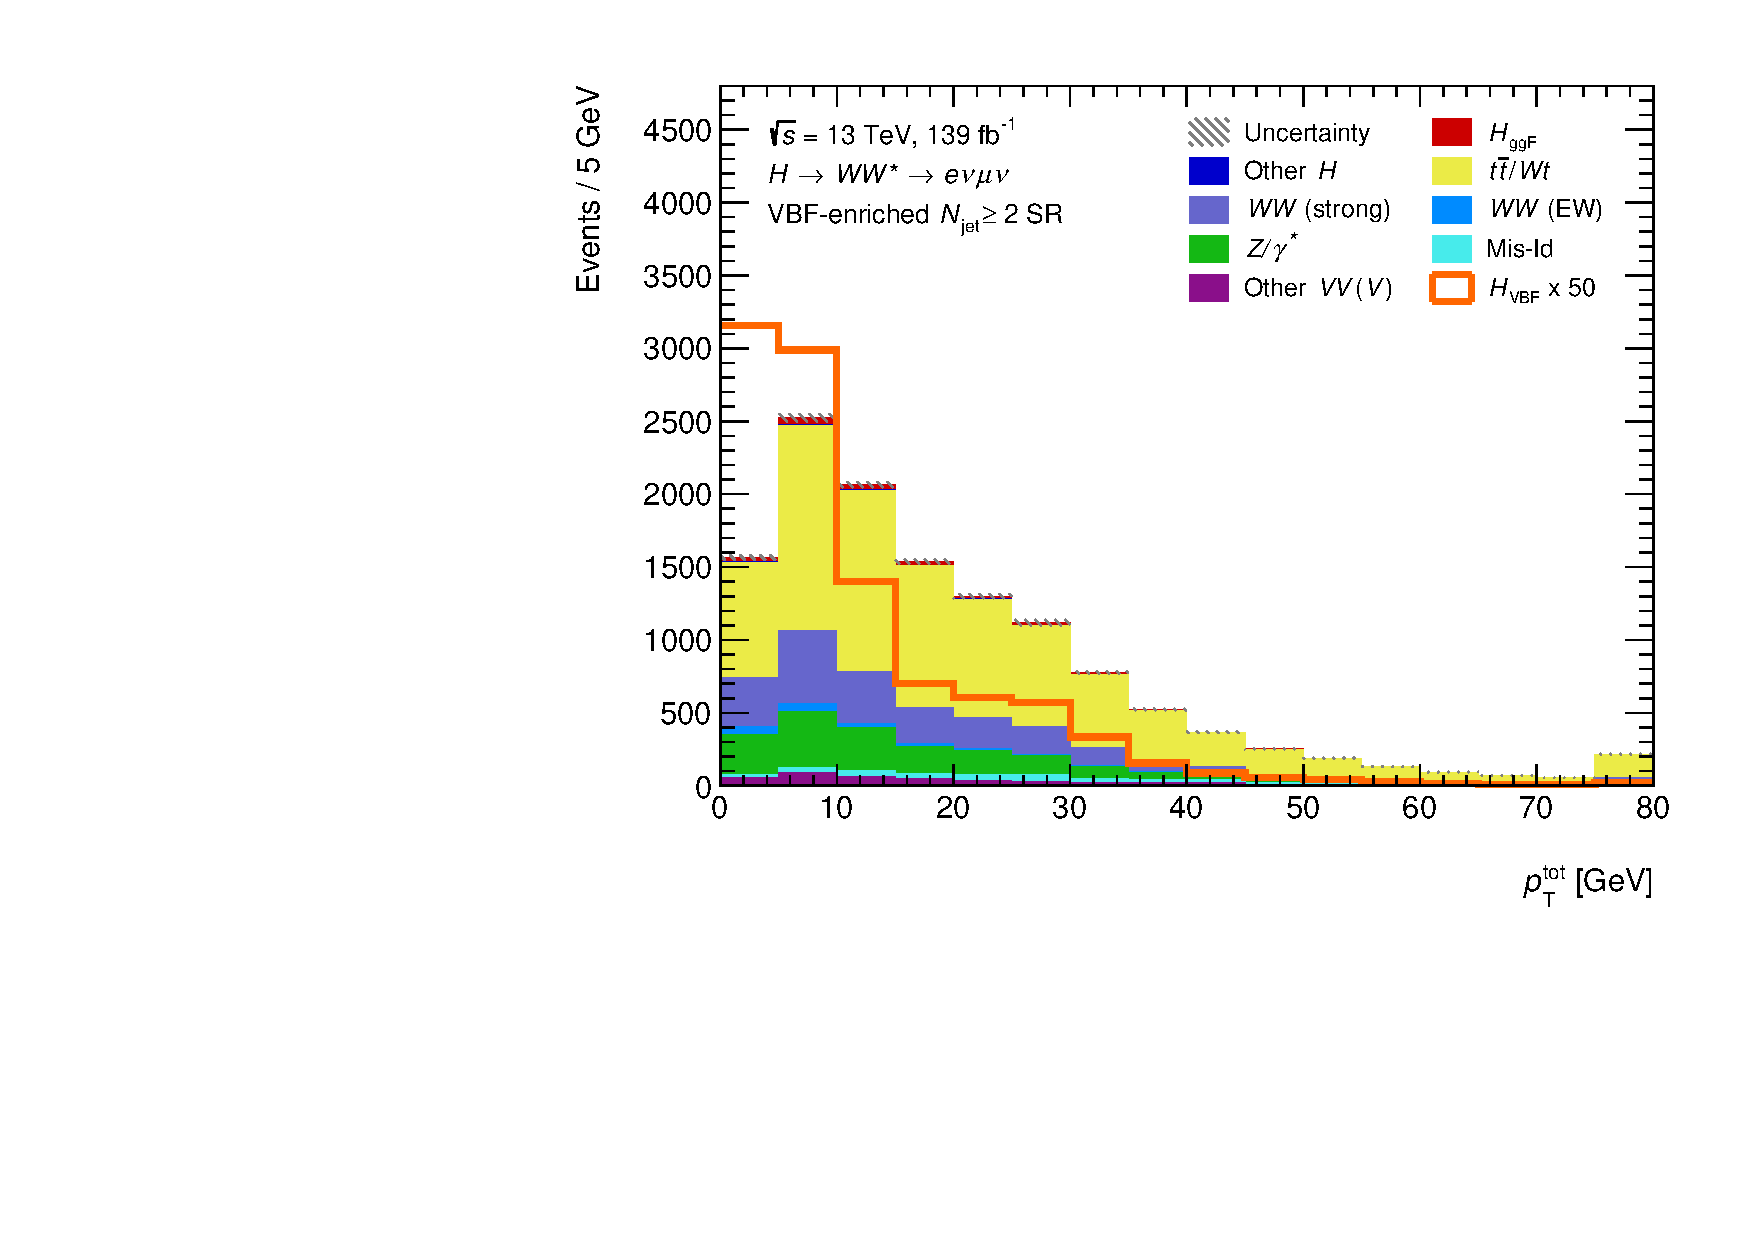
\includegraphics[width=0.32\textwidth]{figures/hww/dnn/blinded/run2-emme-CutVBF_SR-PtTot-lin.pdf} \hfill
        \label{fig:dnn-inputs-post-fit2-4}
    } 
    \subfloat[$\METSig$]{
        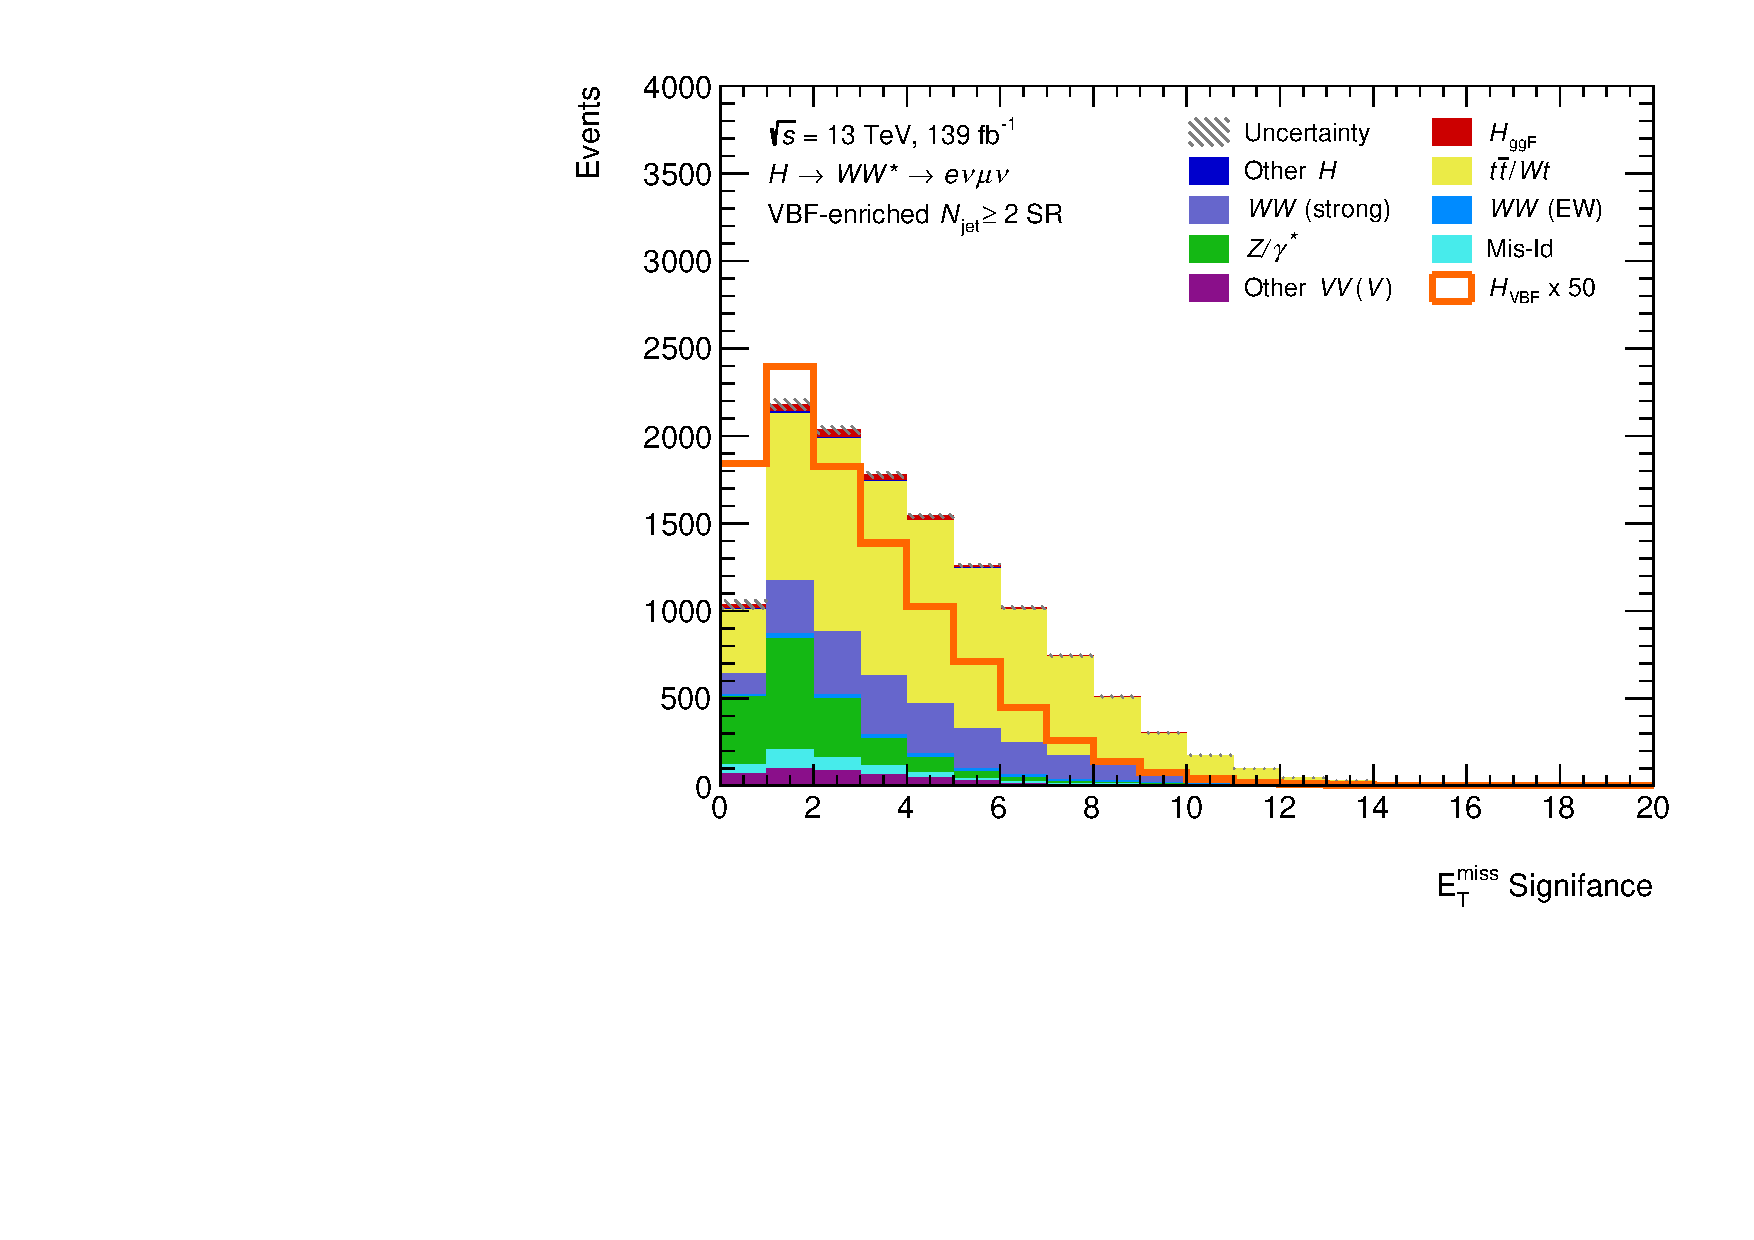
\includegraphics[width=0.32\textwidth]{figures/hww/dnn/blinded/run2-emme-CutVBF_SR-METSig_broad-lin.pdf} \hfill
        \label{fig:dnn-inputs-post-fit2-5}
    } 
    {\caption{Distributions of $\dphill$, $\mll$, $\mT$ in the VBF signal region.
        Each row corresponds to one variable with different selections made on the DNN output.
        \label{fig:dnn-inputs-post-fit2} }}
\end{figure}
}


\newcommand{\dnnfigures}{
\begin{figure}[h]
    \centering
    \subfloat[$\mjj$]{
        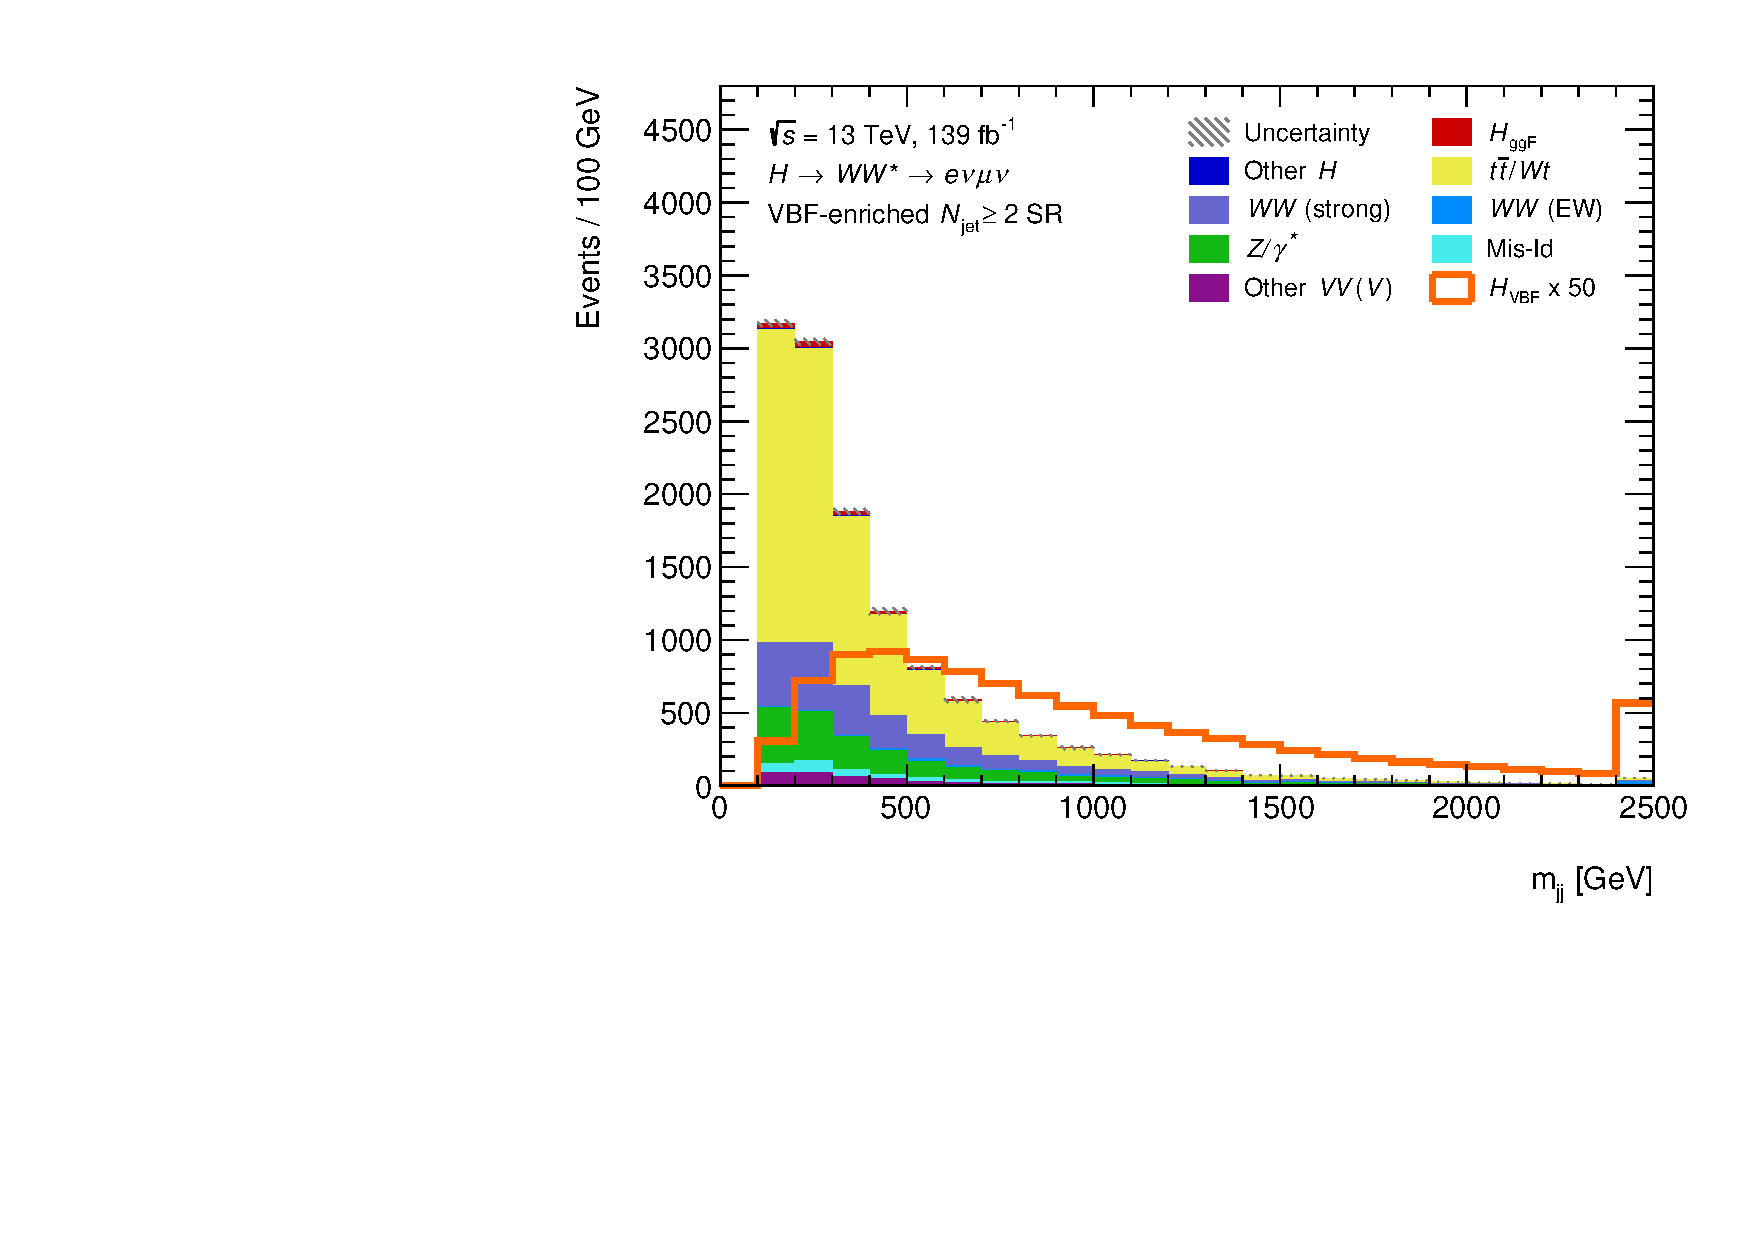
\includegraphics[width=0.32\textwidth]{figures/hww/dnn/blinded/run2-emme-CutVBF_SR-Mjj-lin.pdf} \hfill
        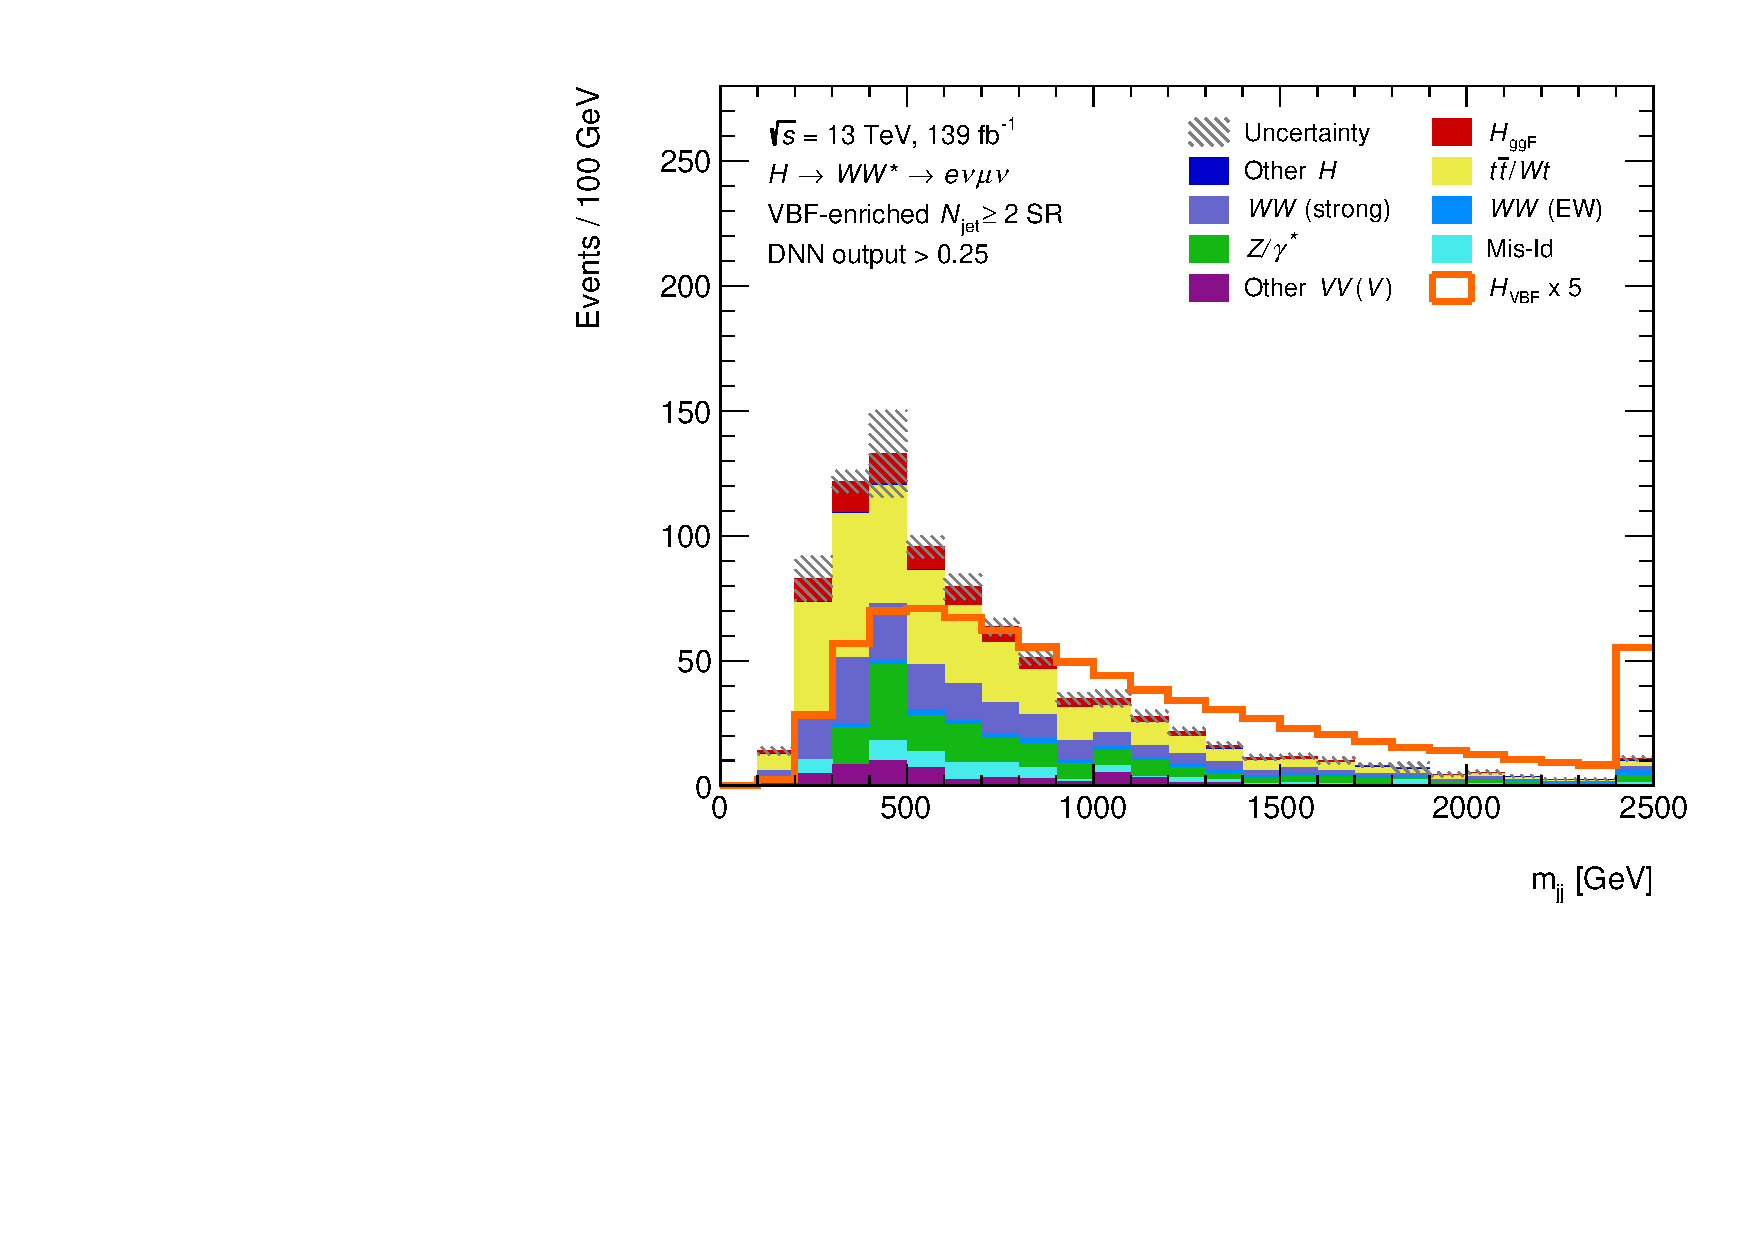
\includegraphics[width=0.32\textwidth]{figures/hww/dnn/blinded/run2-emme-CutVBFSR_DNN25-Mjj-lin.pdf} \hfill
        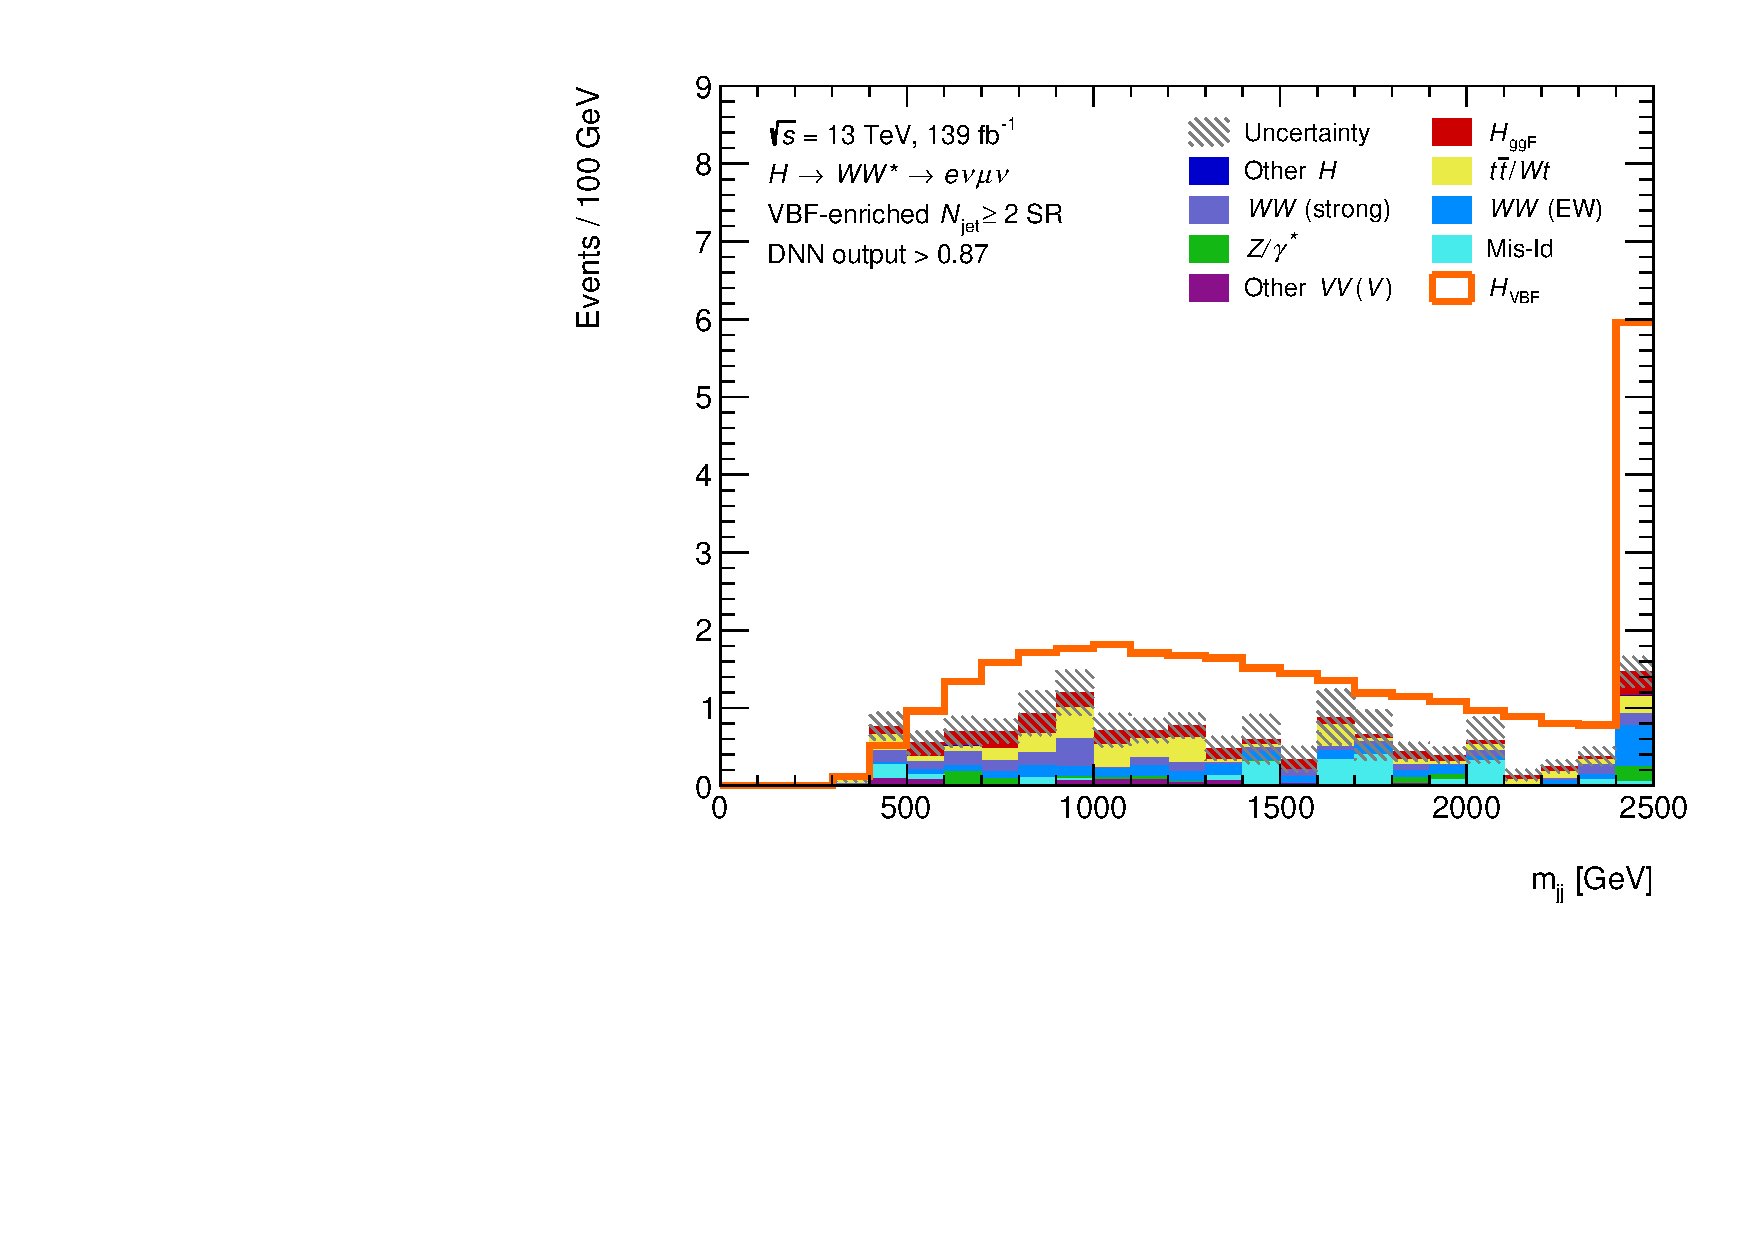
\includegraphics[width=0.32\textwidth]{figures/hww/dnn/blinded/run2-emme-CutVBFSR_DNN87-Mjj-lin.pdf}
    } \\
    \subfloat[$\dyjj$]{
        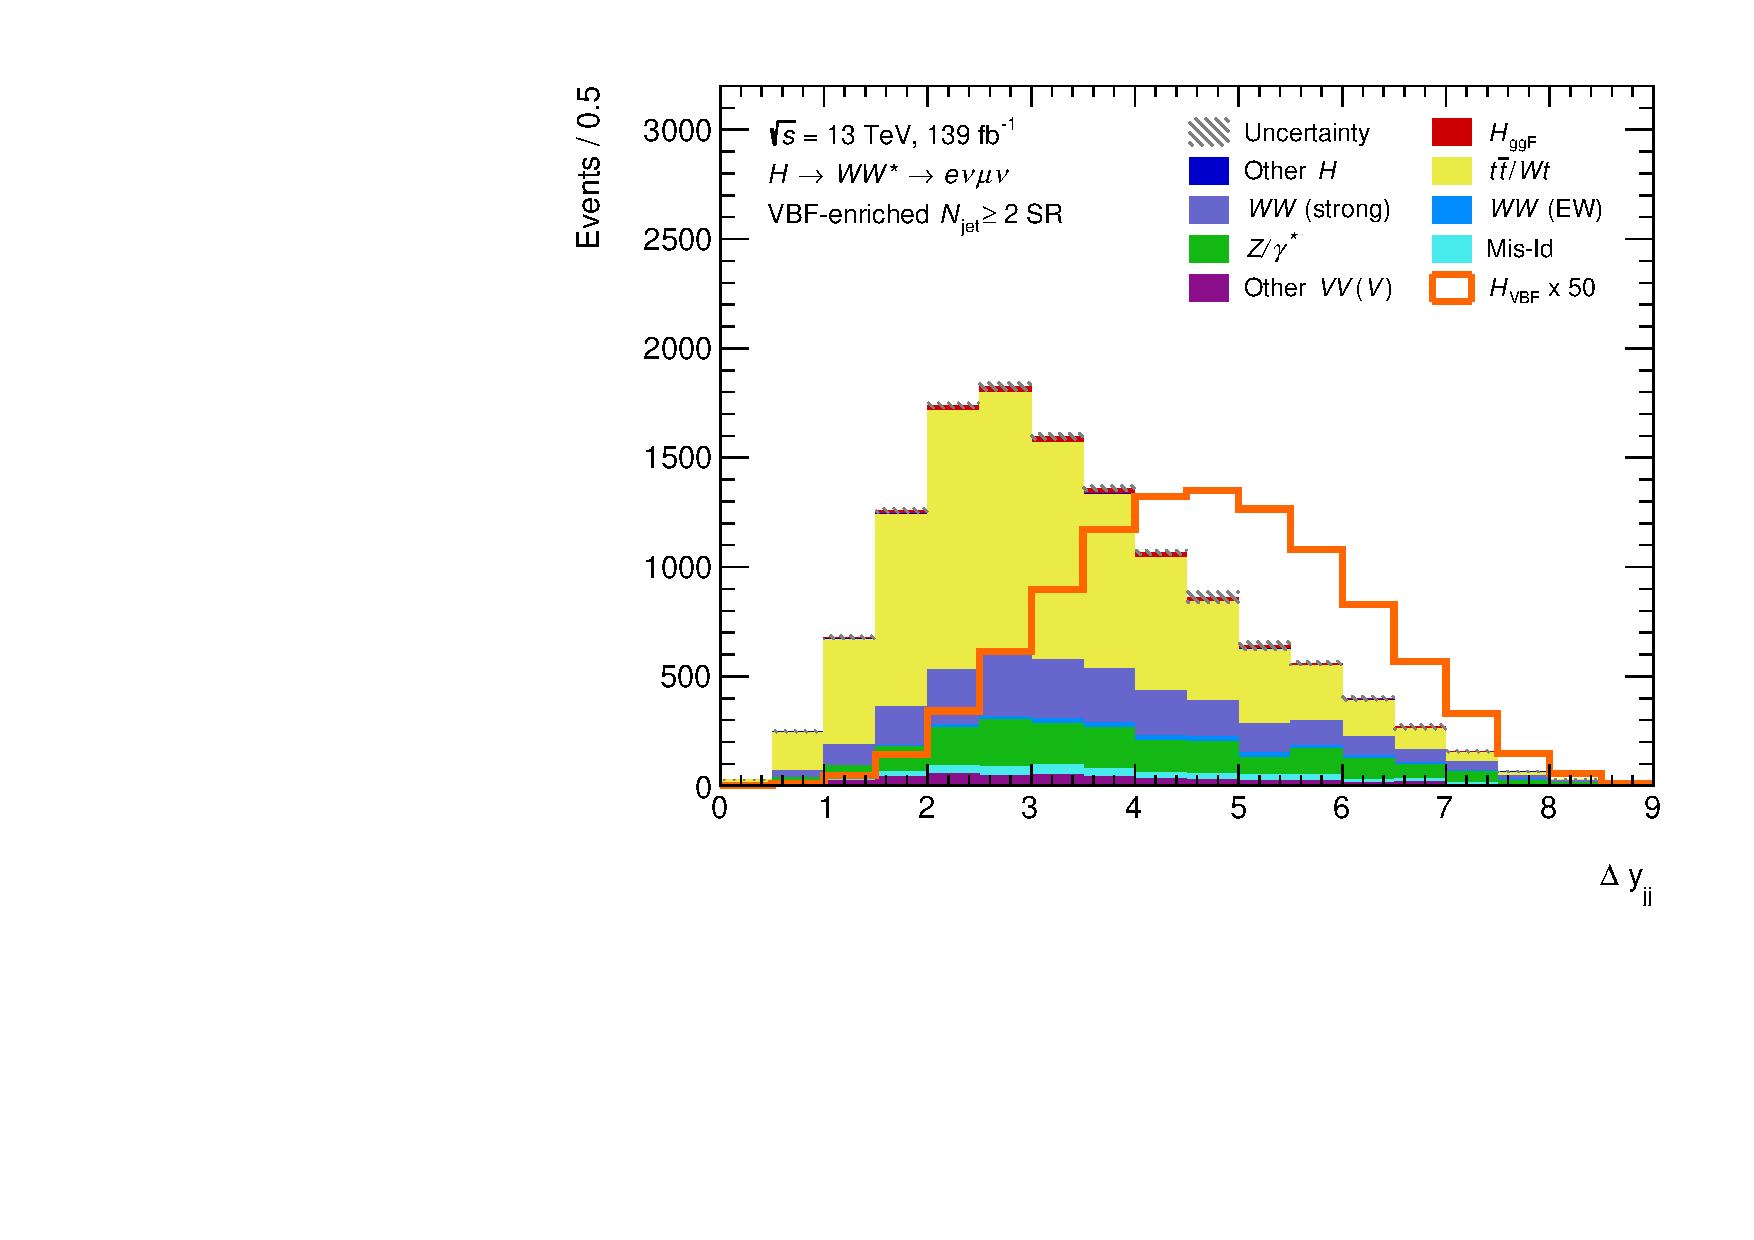
\includegraphics[width=0.32\textwidth]{figures/hww/dnn/blinded/run2-emme-CutVBF_SR-DYjj-lin.pdf} \hfill
        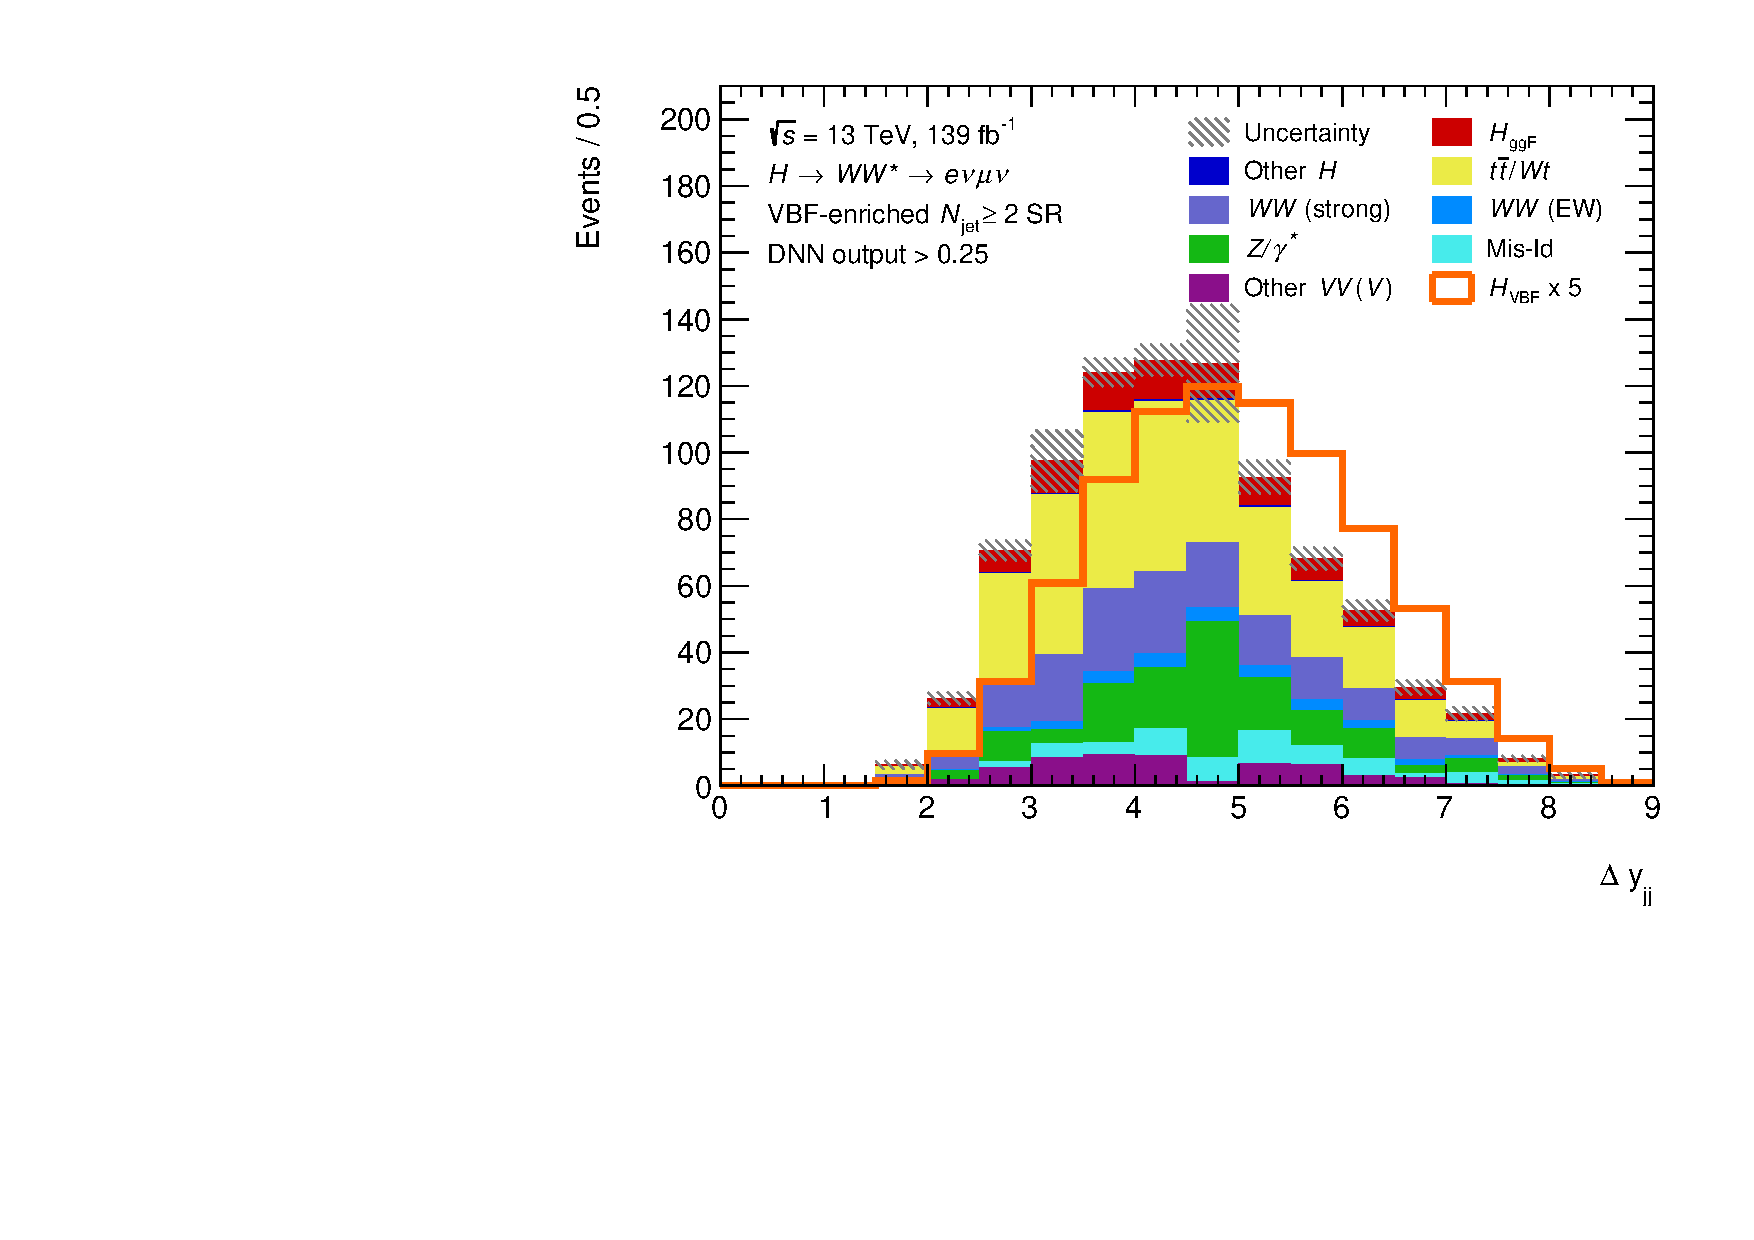
\includegraphics[width=0.32\textwidth]{figures/hww/dnn/blinded/run2-emme-CutVBFSR_DNN25-DYjj-lin.pdf} \hfill
        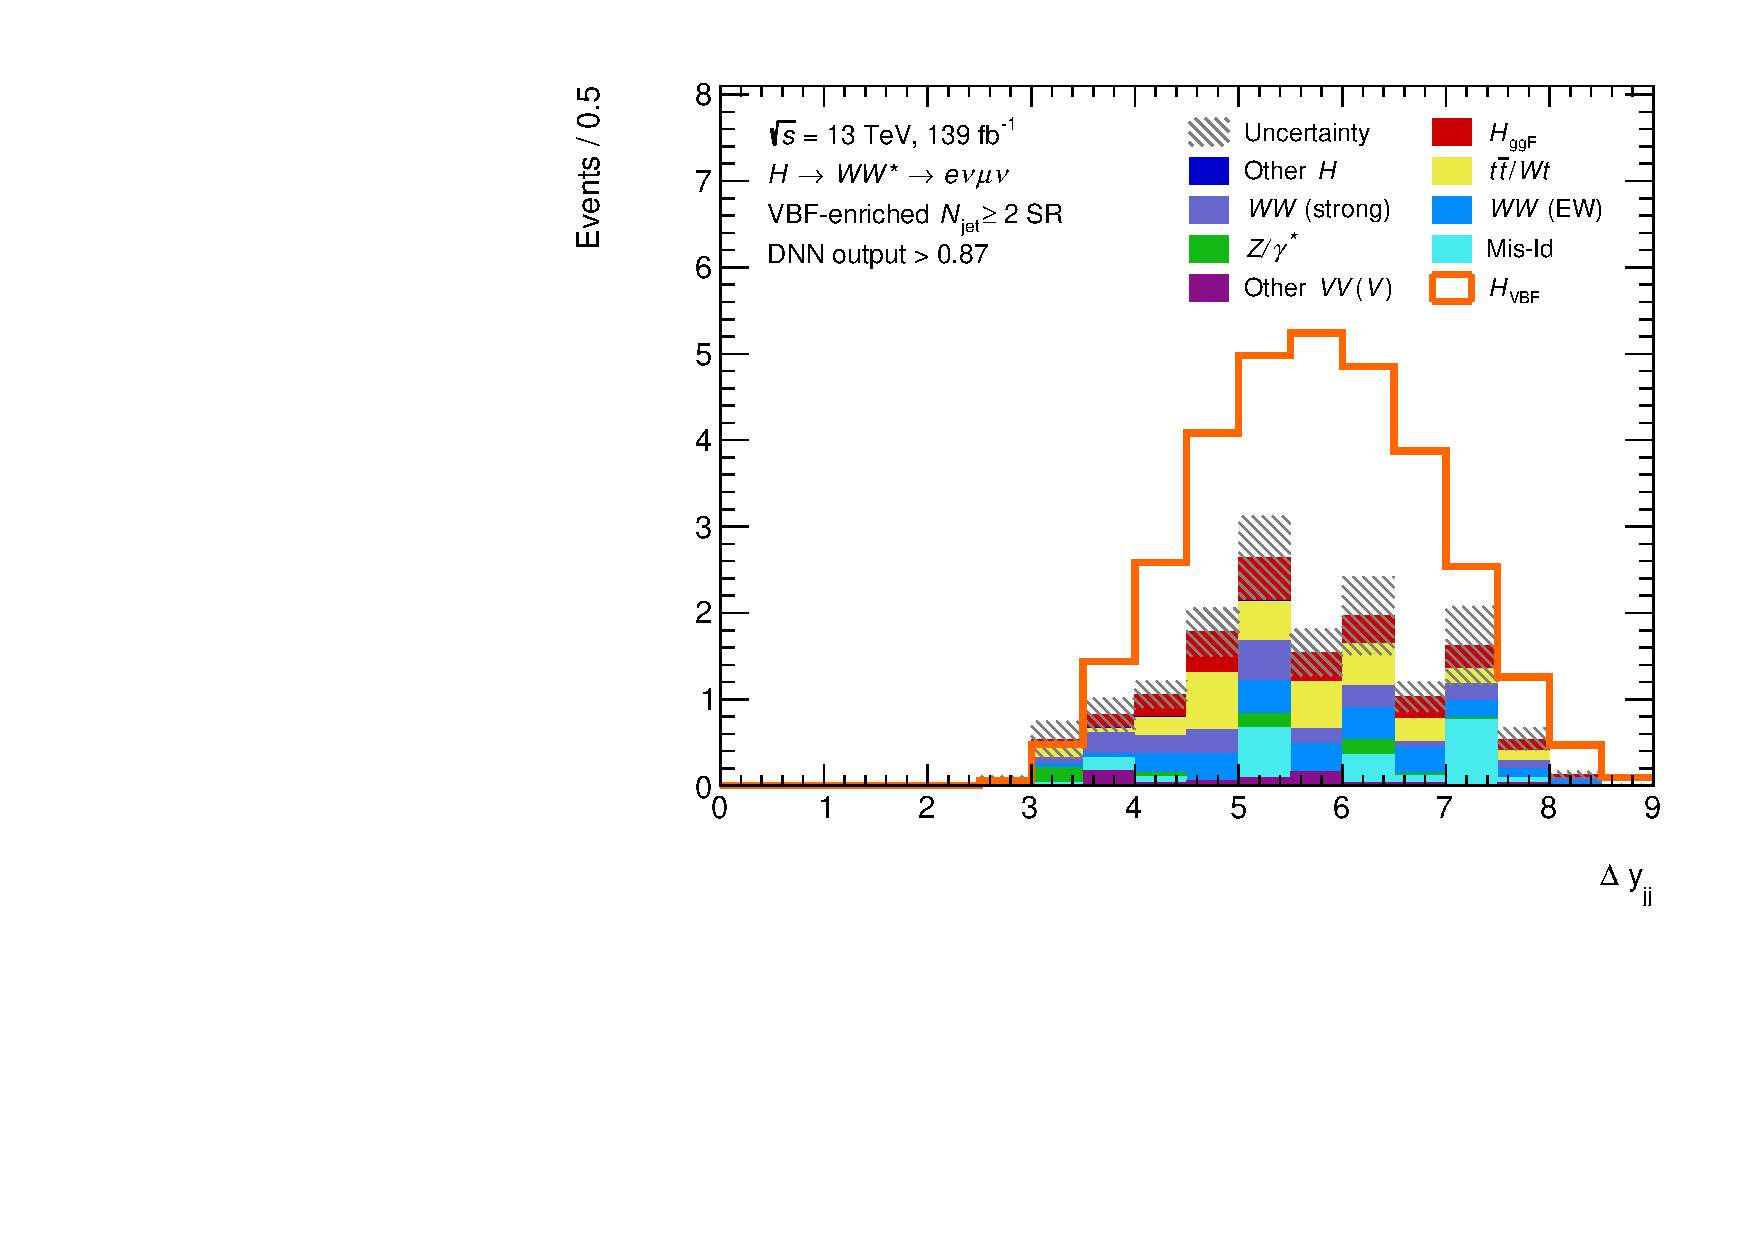
\includegraphics[width=0.32\textwidth]{figures/hww/dnn/blinded/run2-emme-CutVBFSR_DNN87-DYjj-lin.pdf}
    } \\
    \subfloat[$\lepetacent$]{
        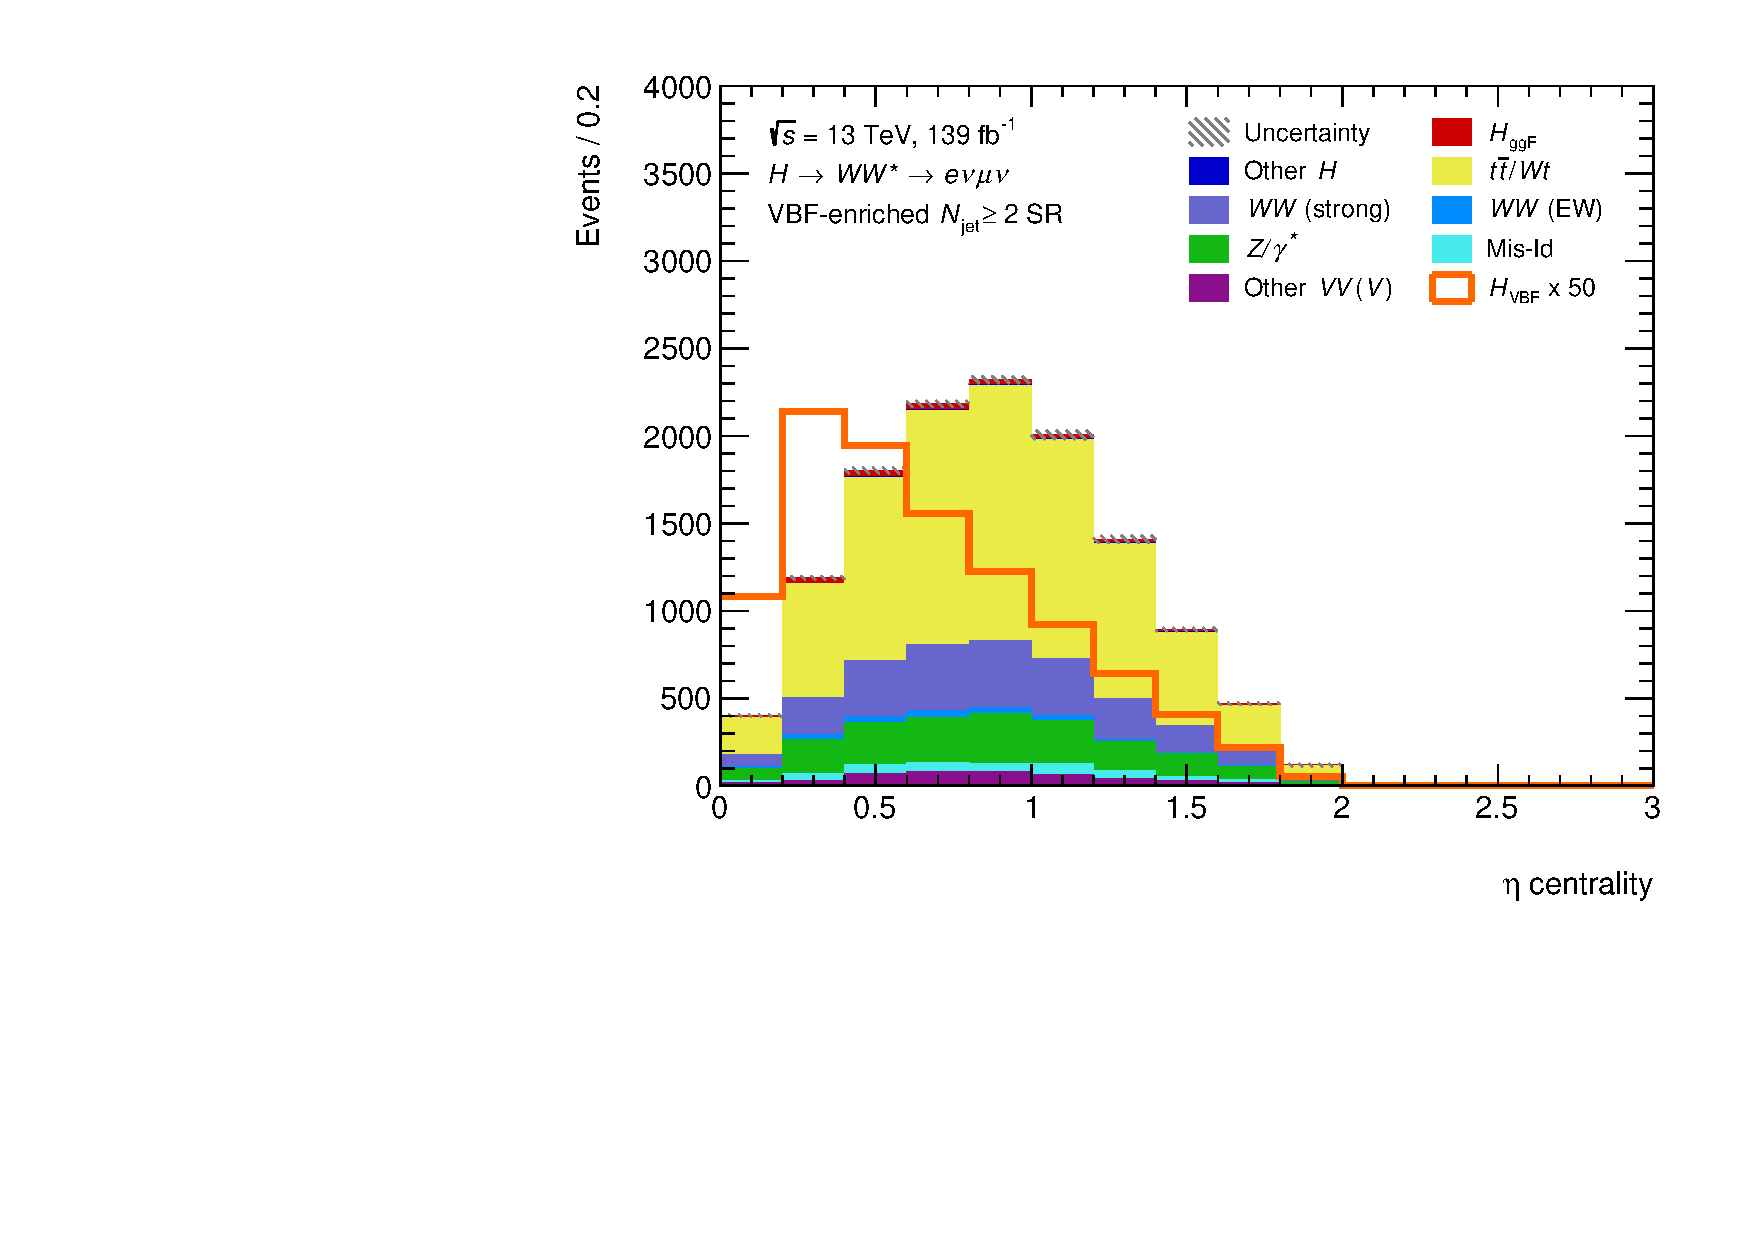
\includegraphics[width=0.32\textwidth]{figures/hww/dnn/blinded/run2-emme-CutVBF_SR-contOLV-lin.pdf} \hfill
        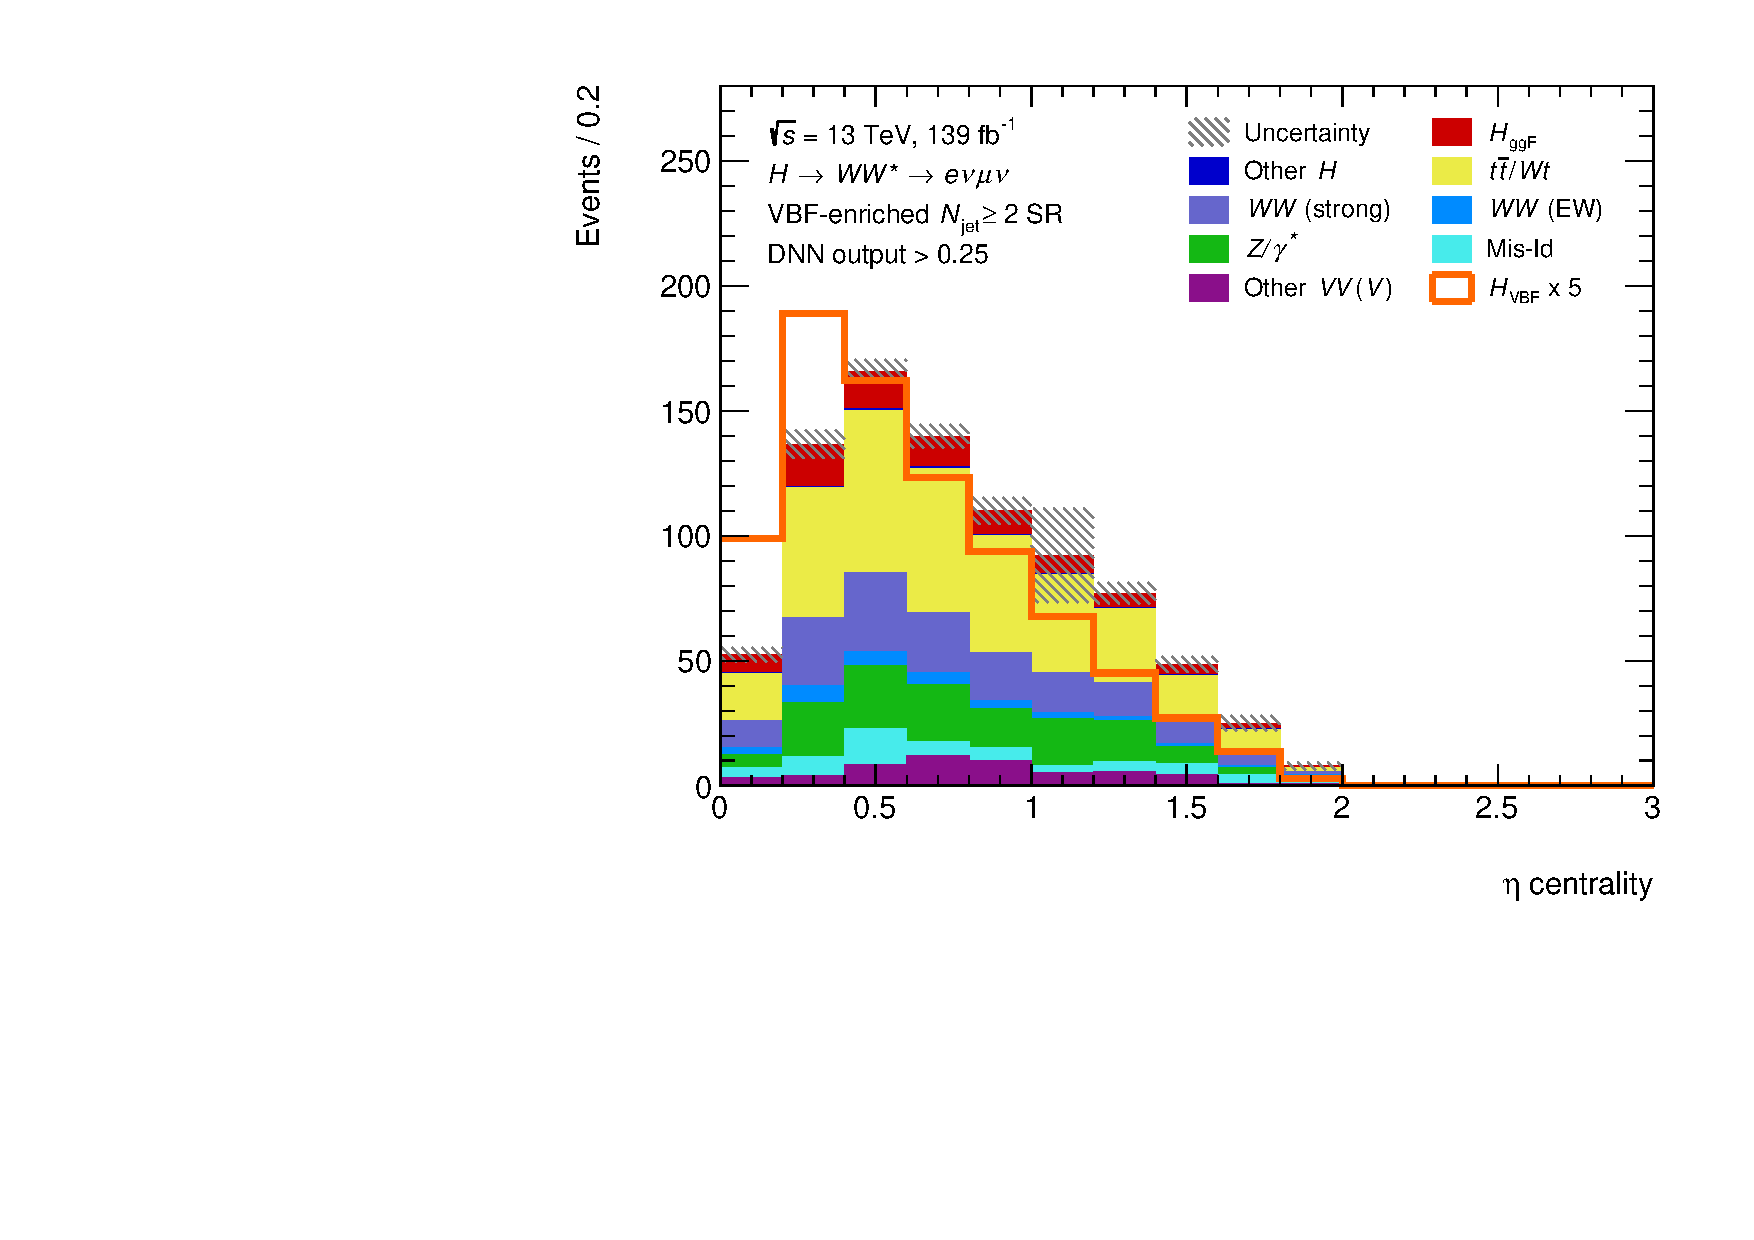
\includegraphics[width=0.32\textwidth]{figures/hww/dnn/blinded/run2-emme-CutVBFSR_DNN25-contOLV-lin.pdf} \hfill
        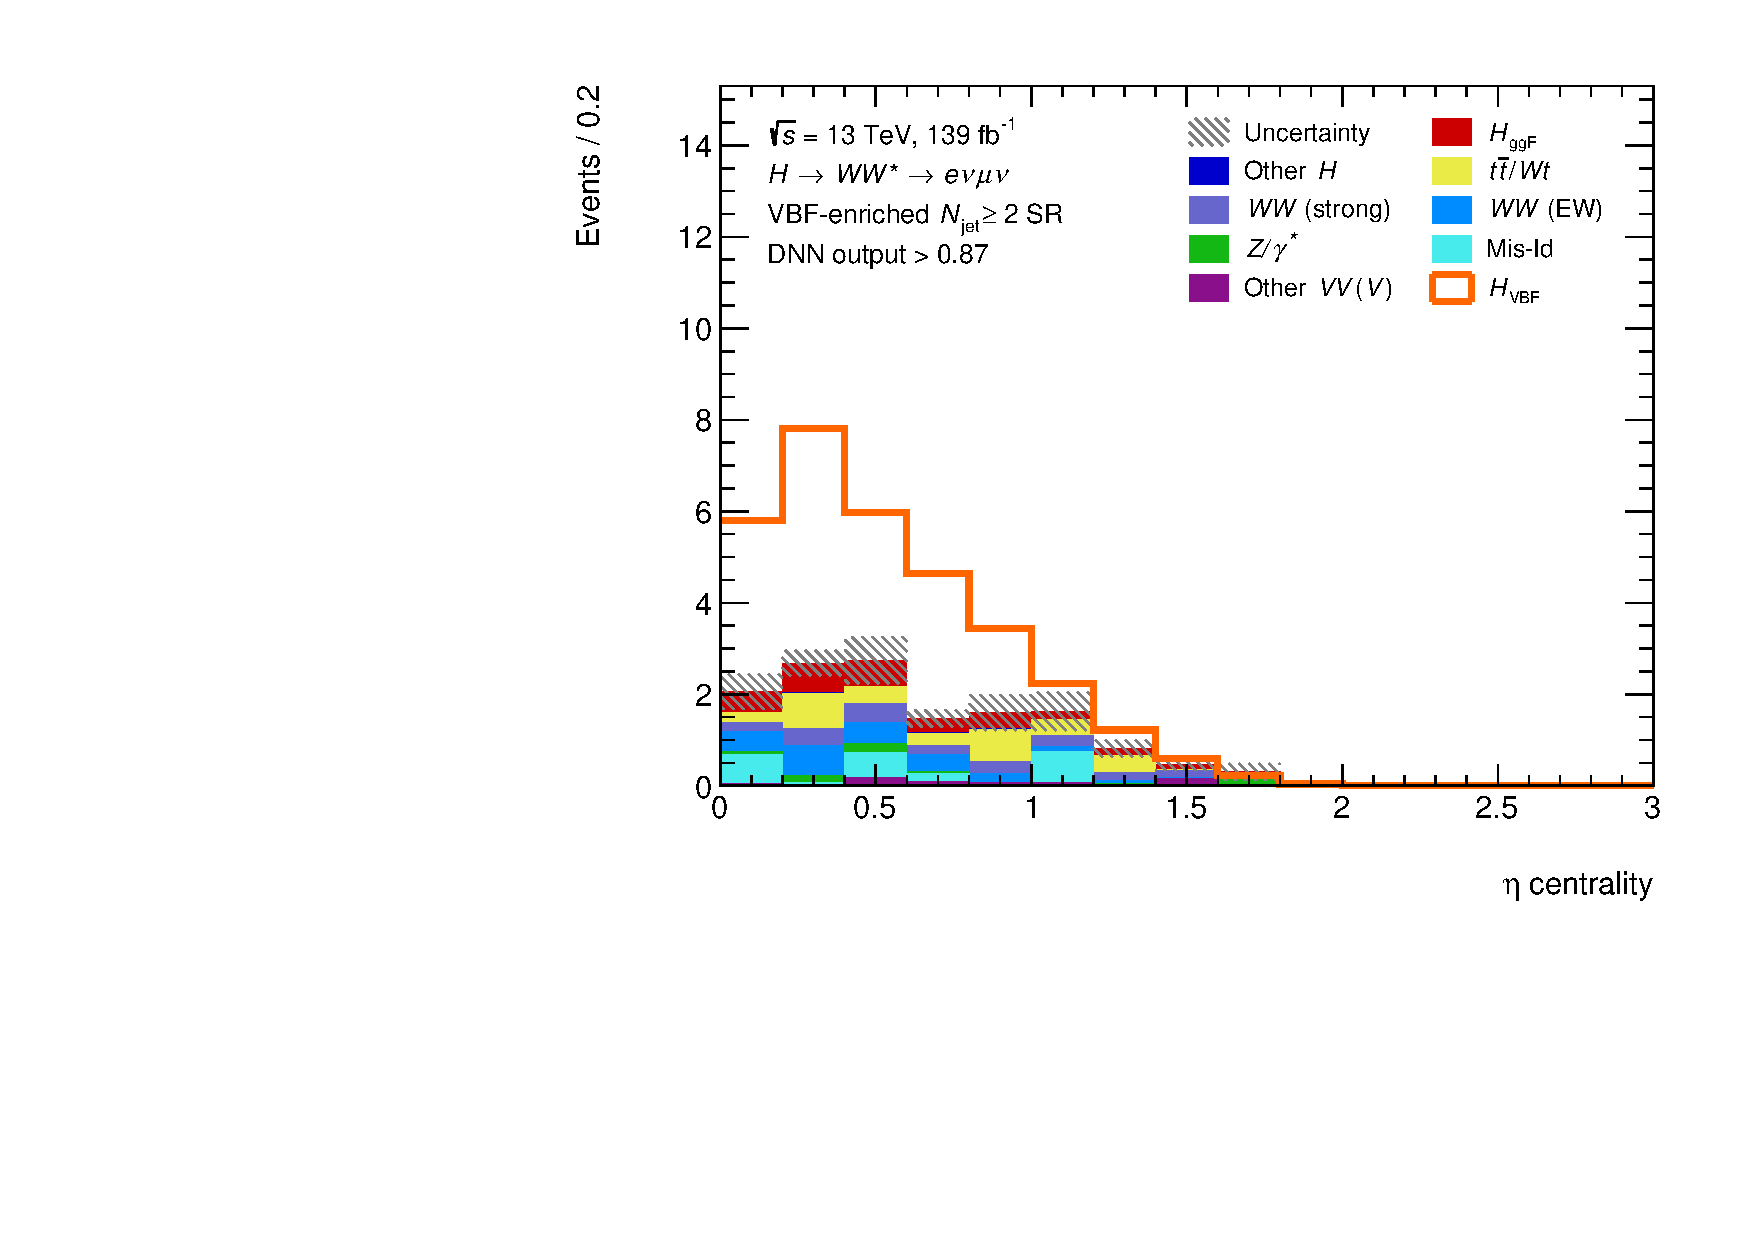
\includegraphics[width=0.32\textwidth]{figures/hww/dnn/blinded/run2-emme-CutVBFSR_DNN87-contOLV-lin.pdf}
    } \\
    {\caption{Distributions of $\dphill$, $\mll$, $\lepetacent$ in the VBF signal region.
        Each row corresponds to one variable with different selections made on the DNN output.
        \label{app:fig:dnn-inputs-vbf-top1} }}
\end{figure}


\begin{figure}[h]
    \centering
    \subfloat[$\mlonejtwo$]{
        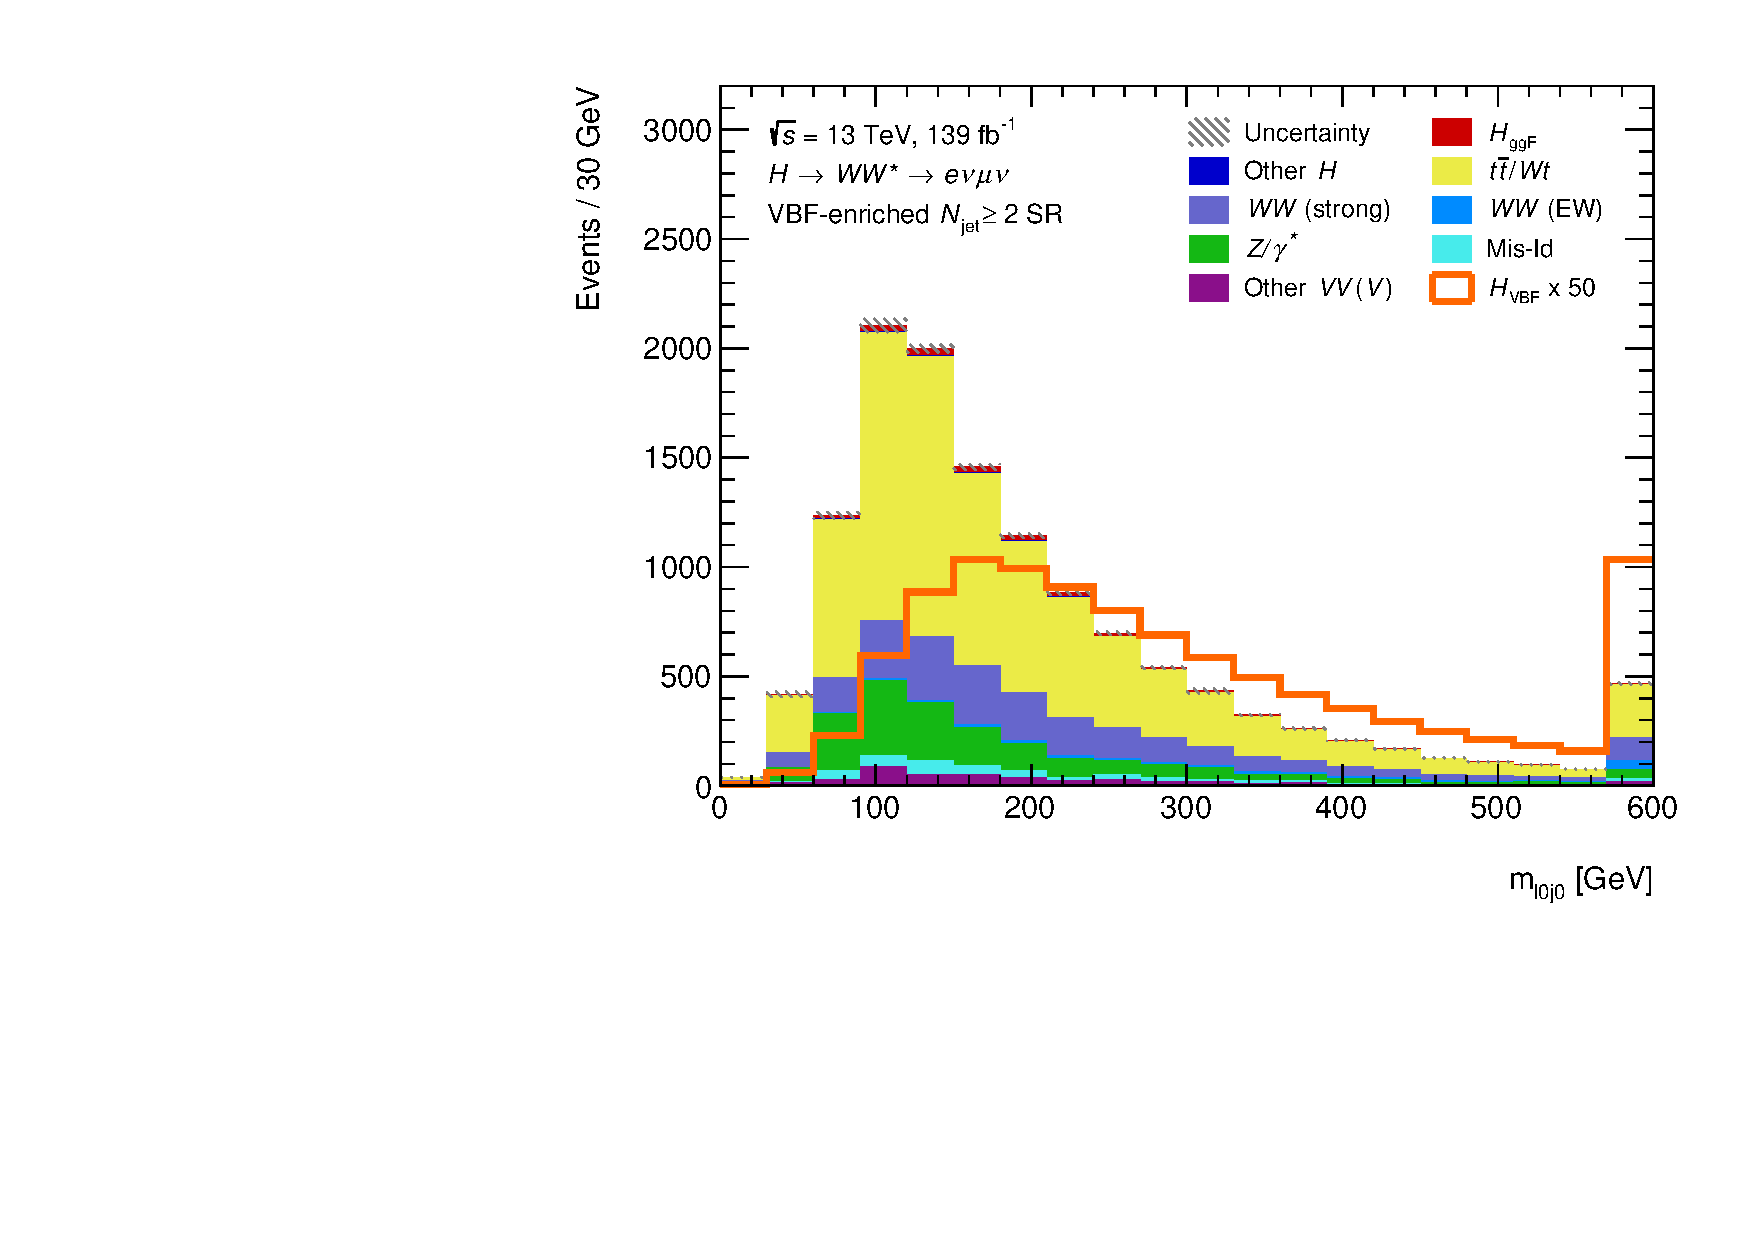
\includegraphics[width=0.32\textwidth]{figures/hww/dnn/blinded/run2-emme-CutVBF_SR-Ml0j0-lin.pdf} \hfill
        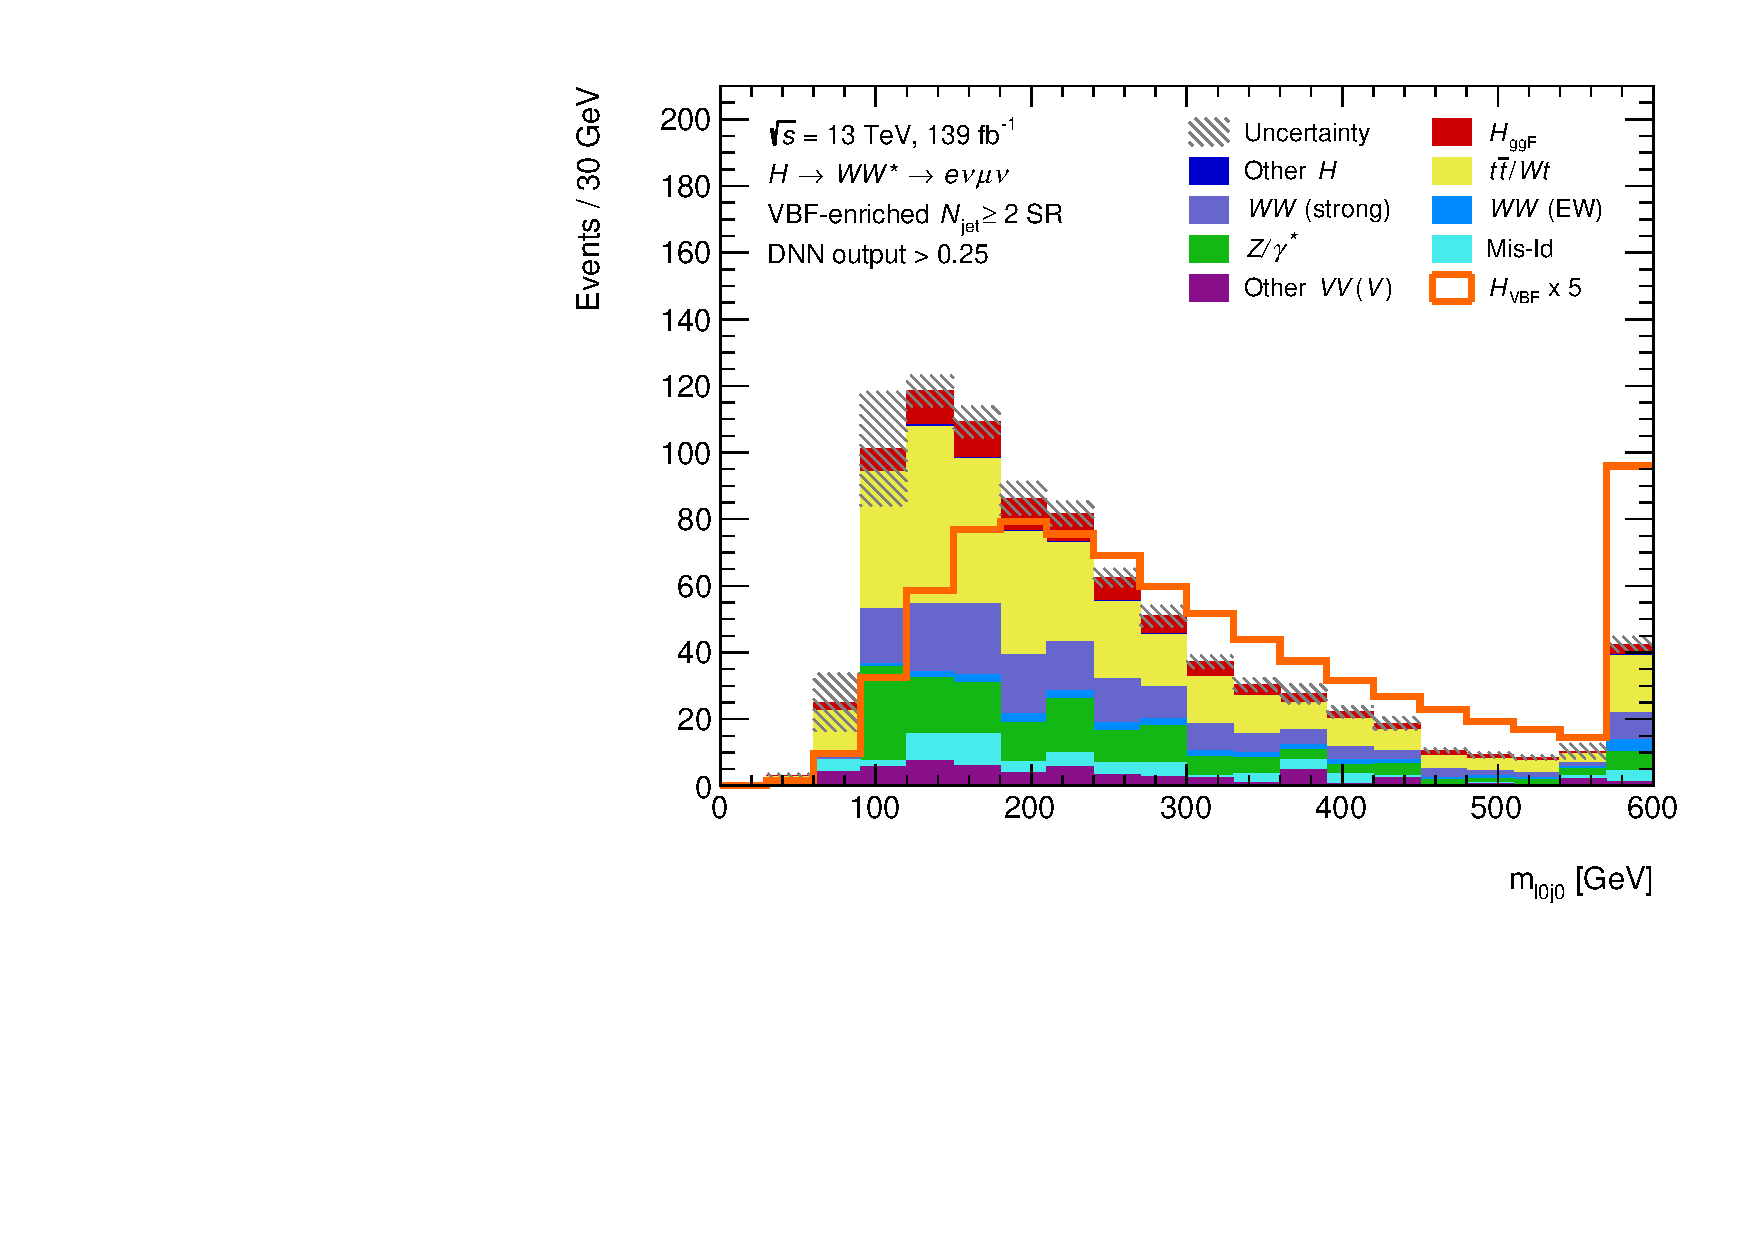
\includegraphics[width=0.32\textwidth]{figures/hww/dnn/blinded/run2-emme-CutVBFSR_DNN25-Ml0j0-lin.pdf} \hfill
        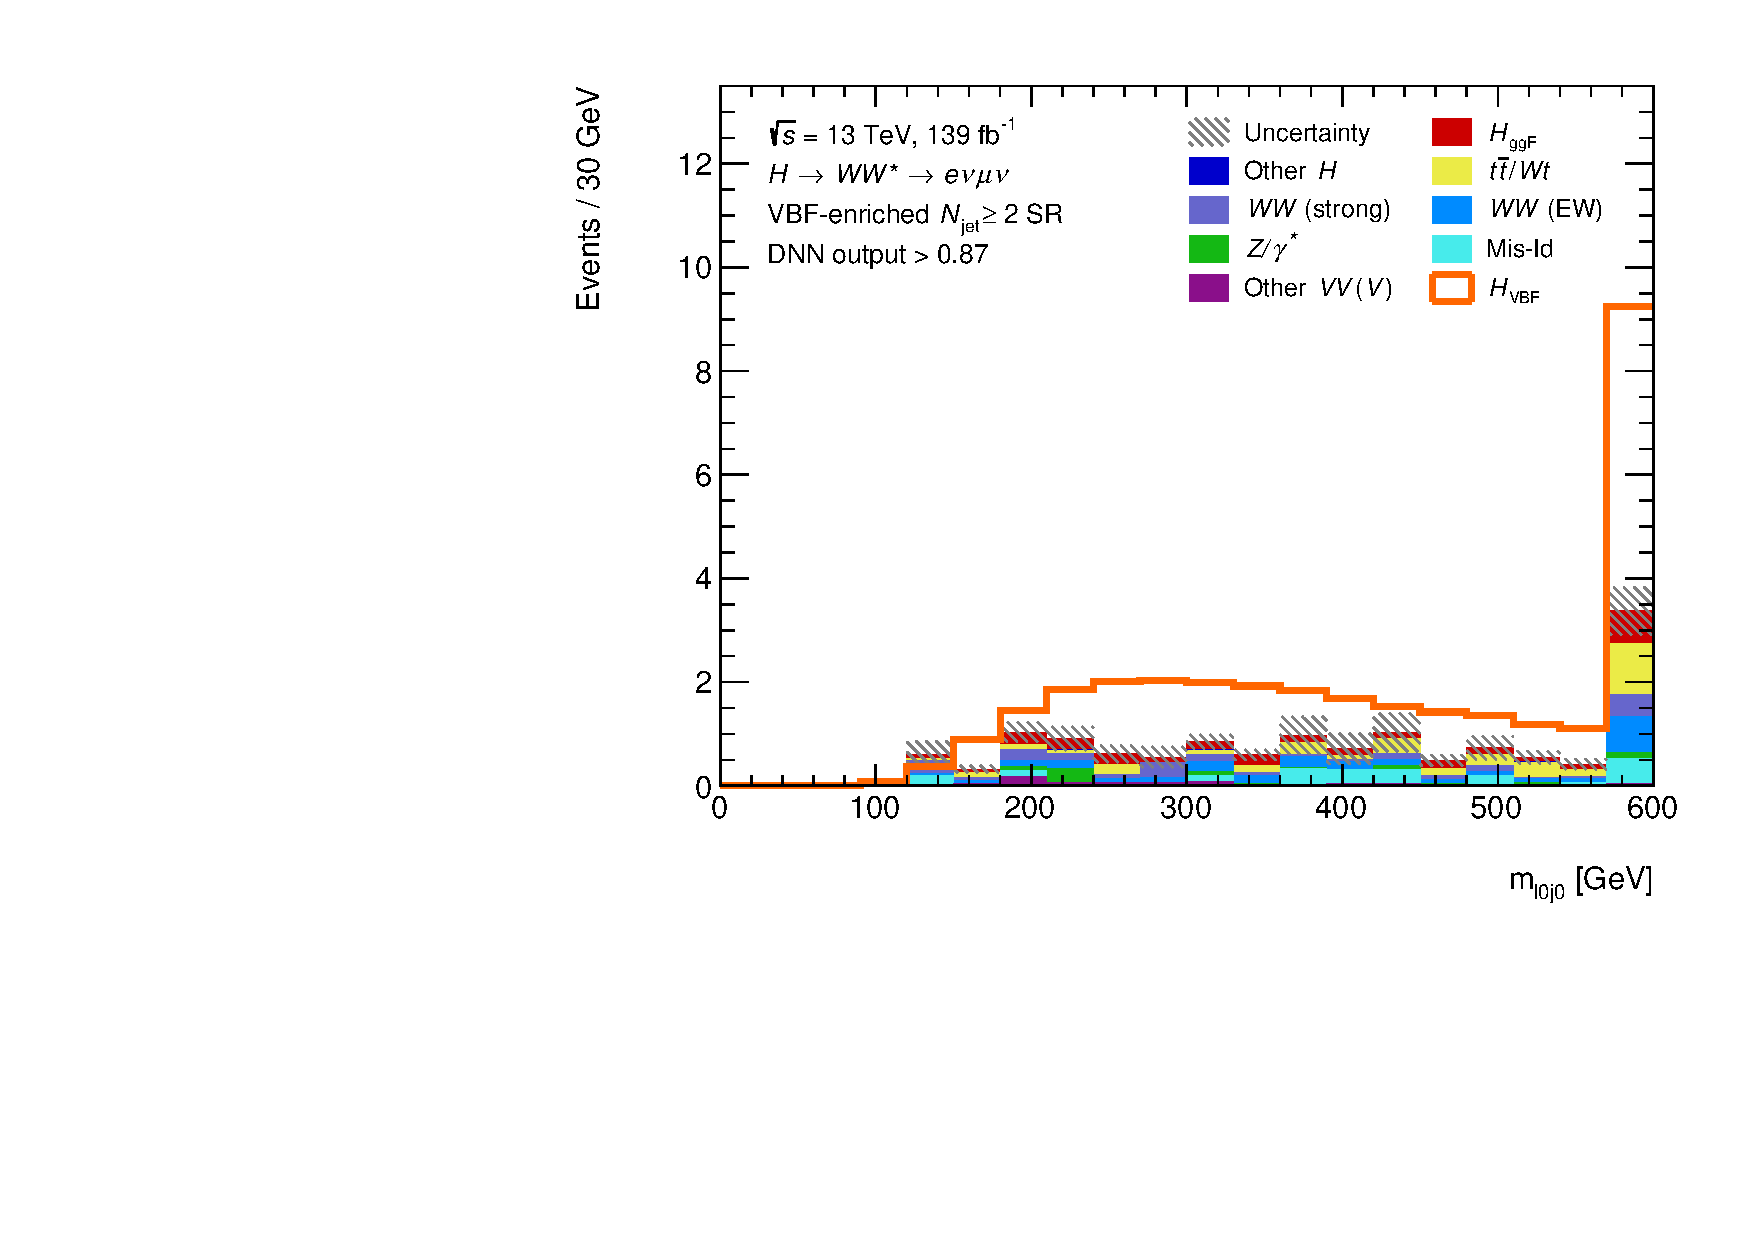
\includegraphics[width=0.32\textwidth]{figures/hww/dnn/blinded/run2-emme-CutVBFSR_DNN87-Ml0j0-lin.pdf}
    } \\
    \subfloat[$\mltwojone$]{
        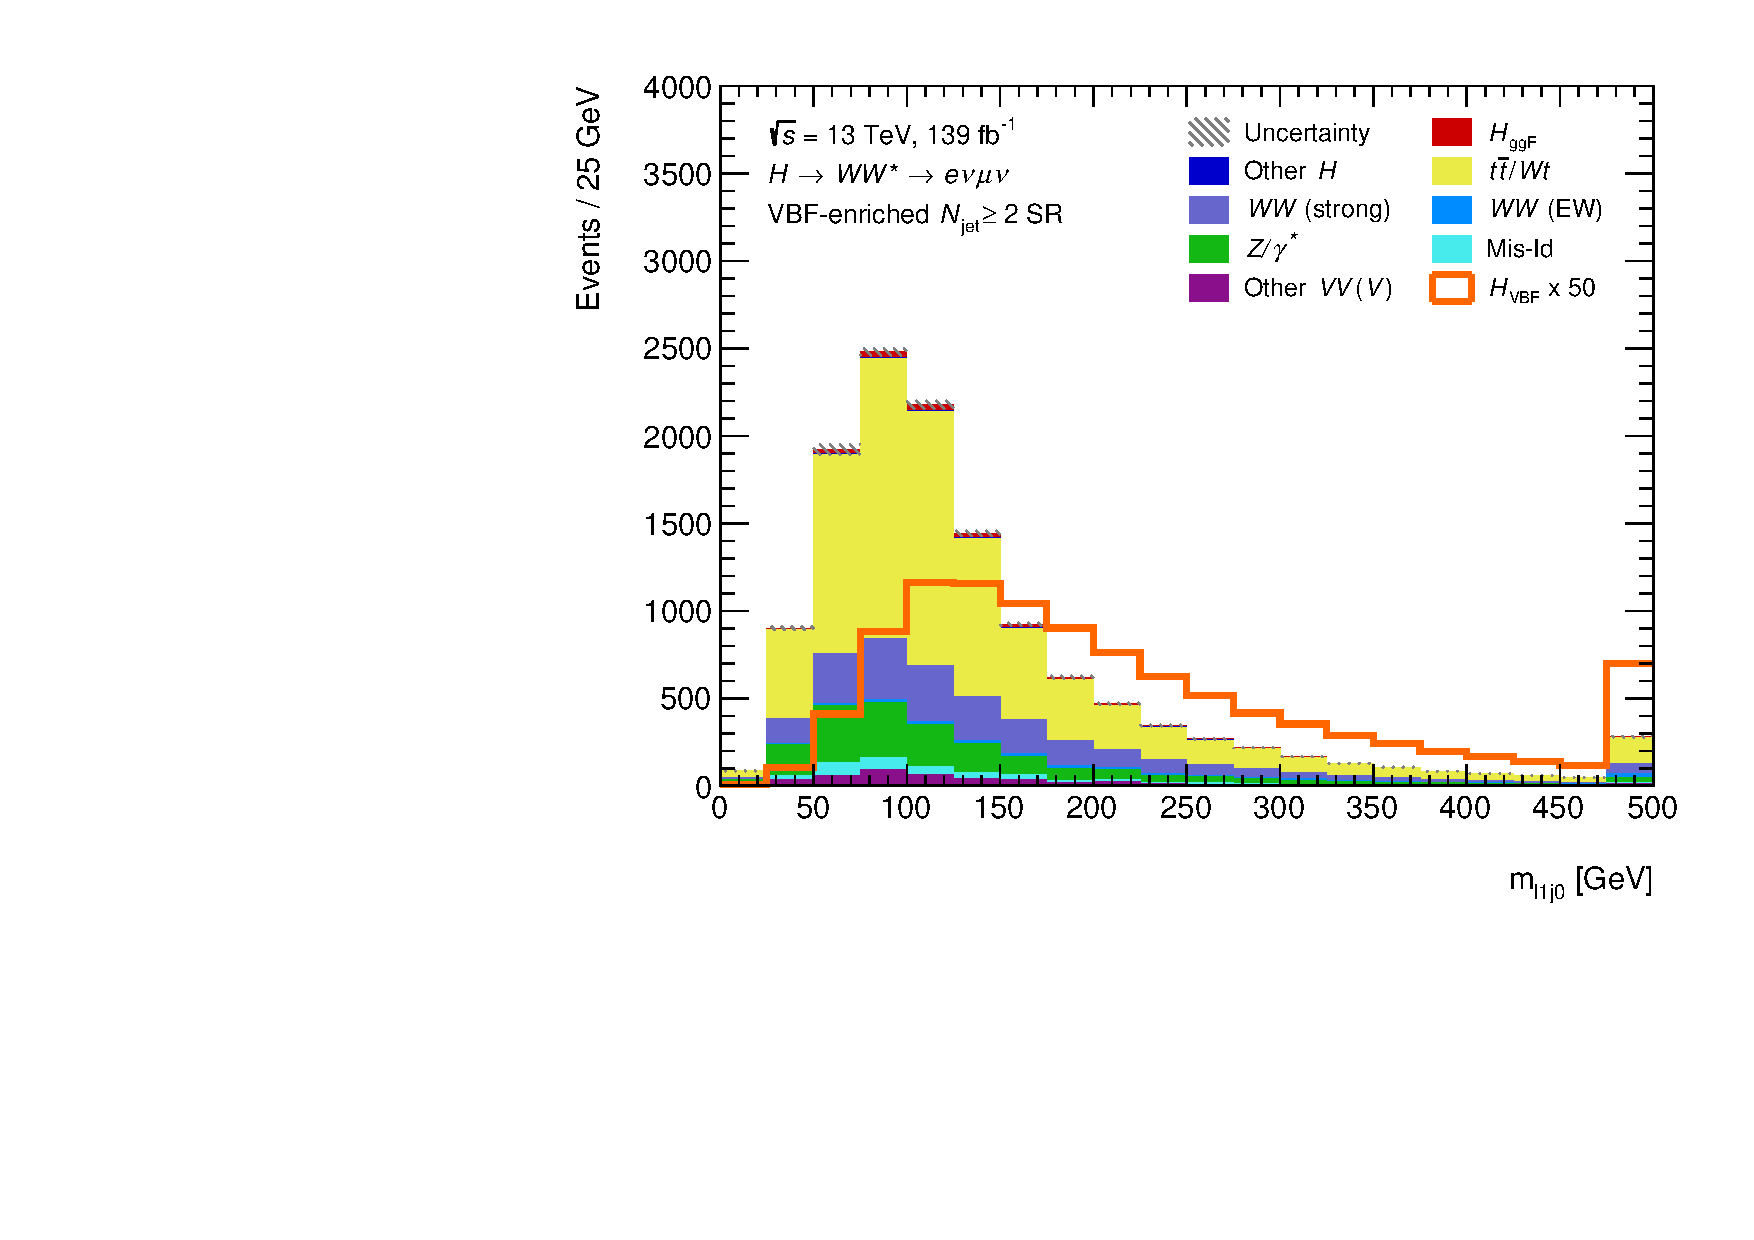
\includegraphics[width=0.32\textwidth]{figures/hww/dnn/blinded/run2-emme-CutVBF_SR-Ml1j0-lin.pdf} \hfill
        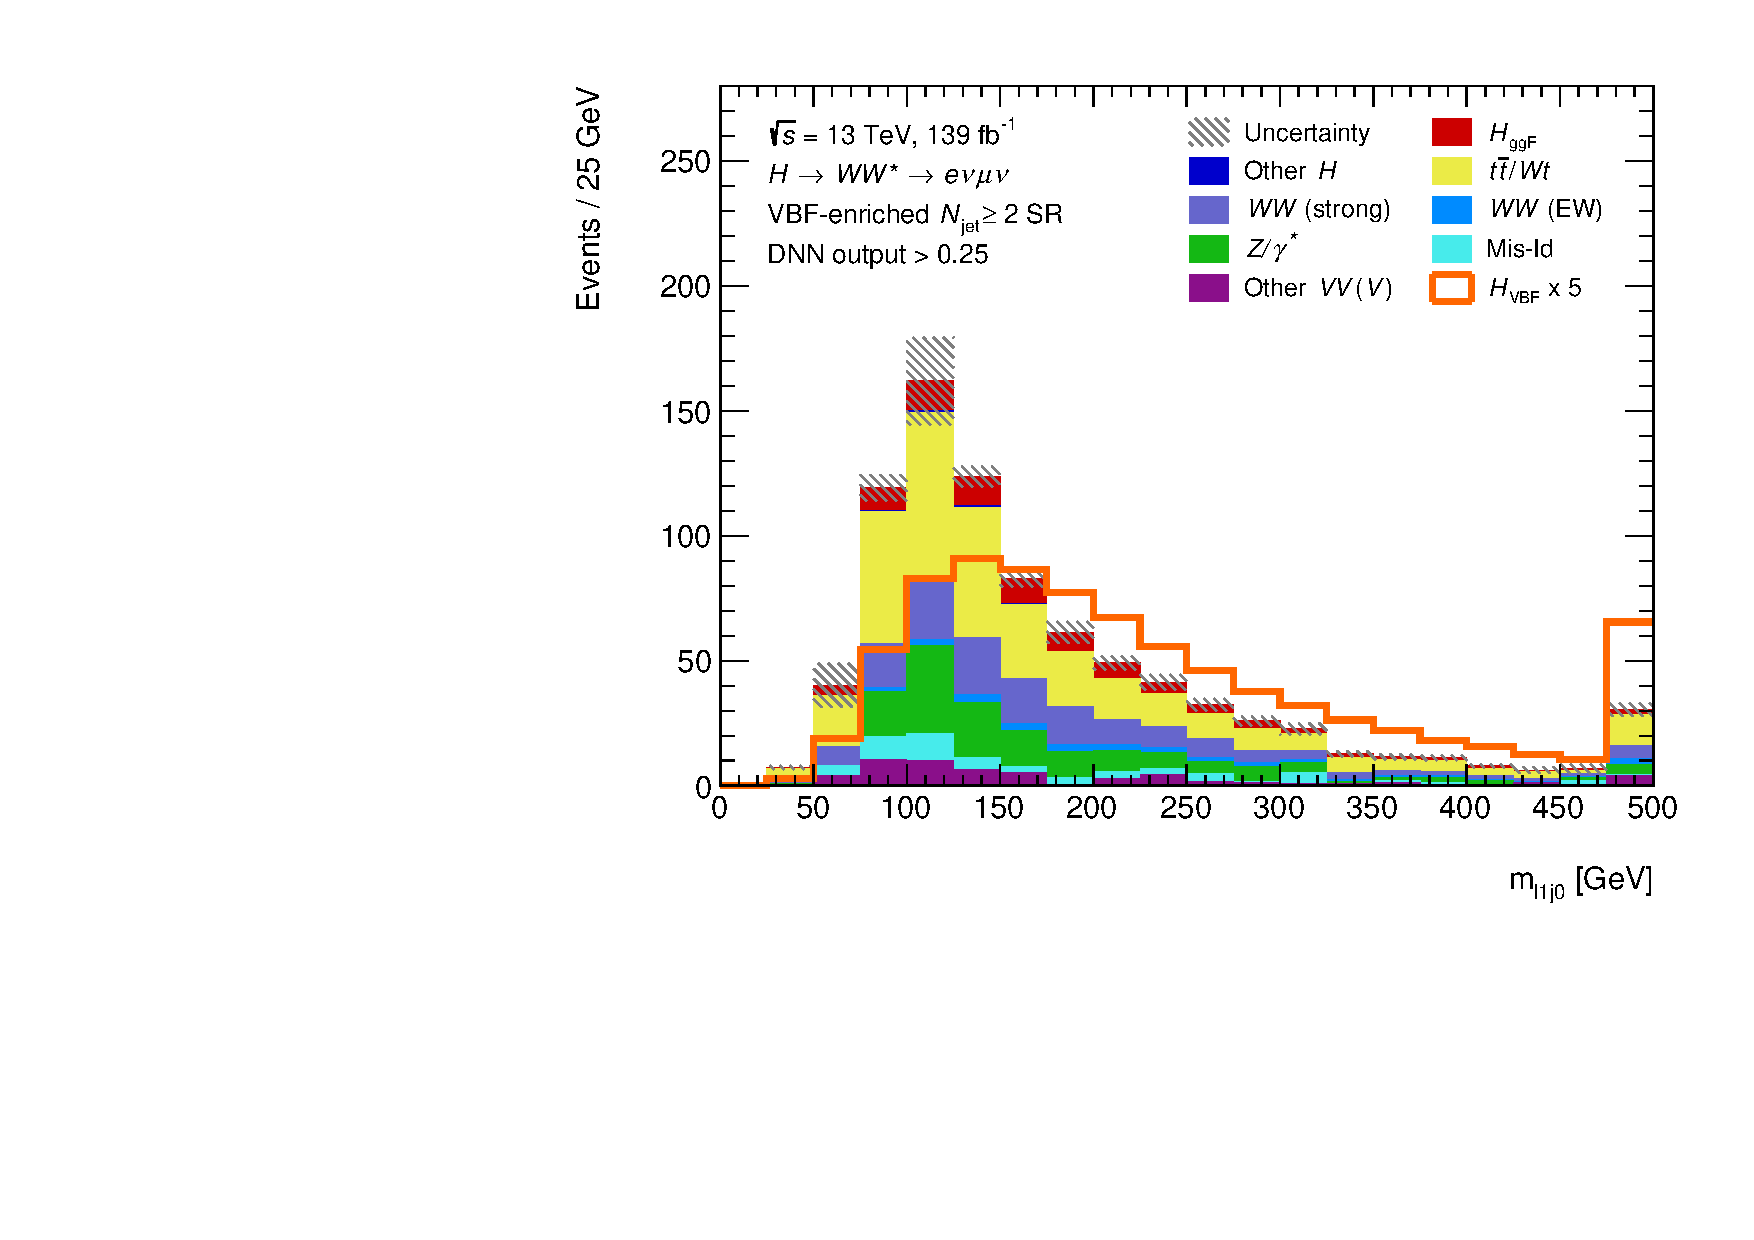
\includegraphics[width=0.32\textwidth]{figures/hww/dnn/blinded/run2-emme-CutVBFSR_DNN25-Ml1j0-lin.pdf} \hfill
        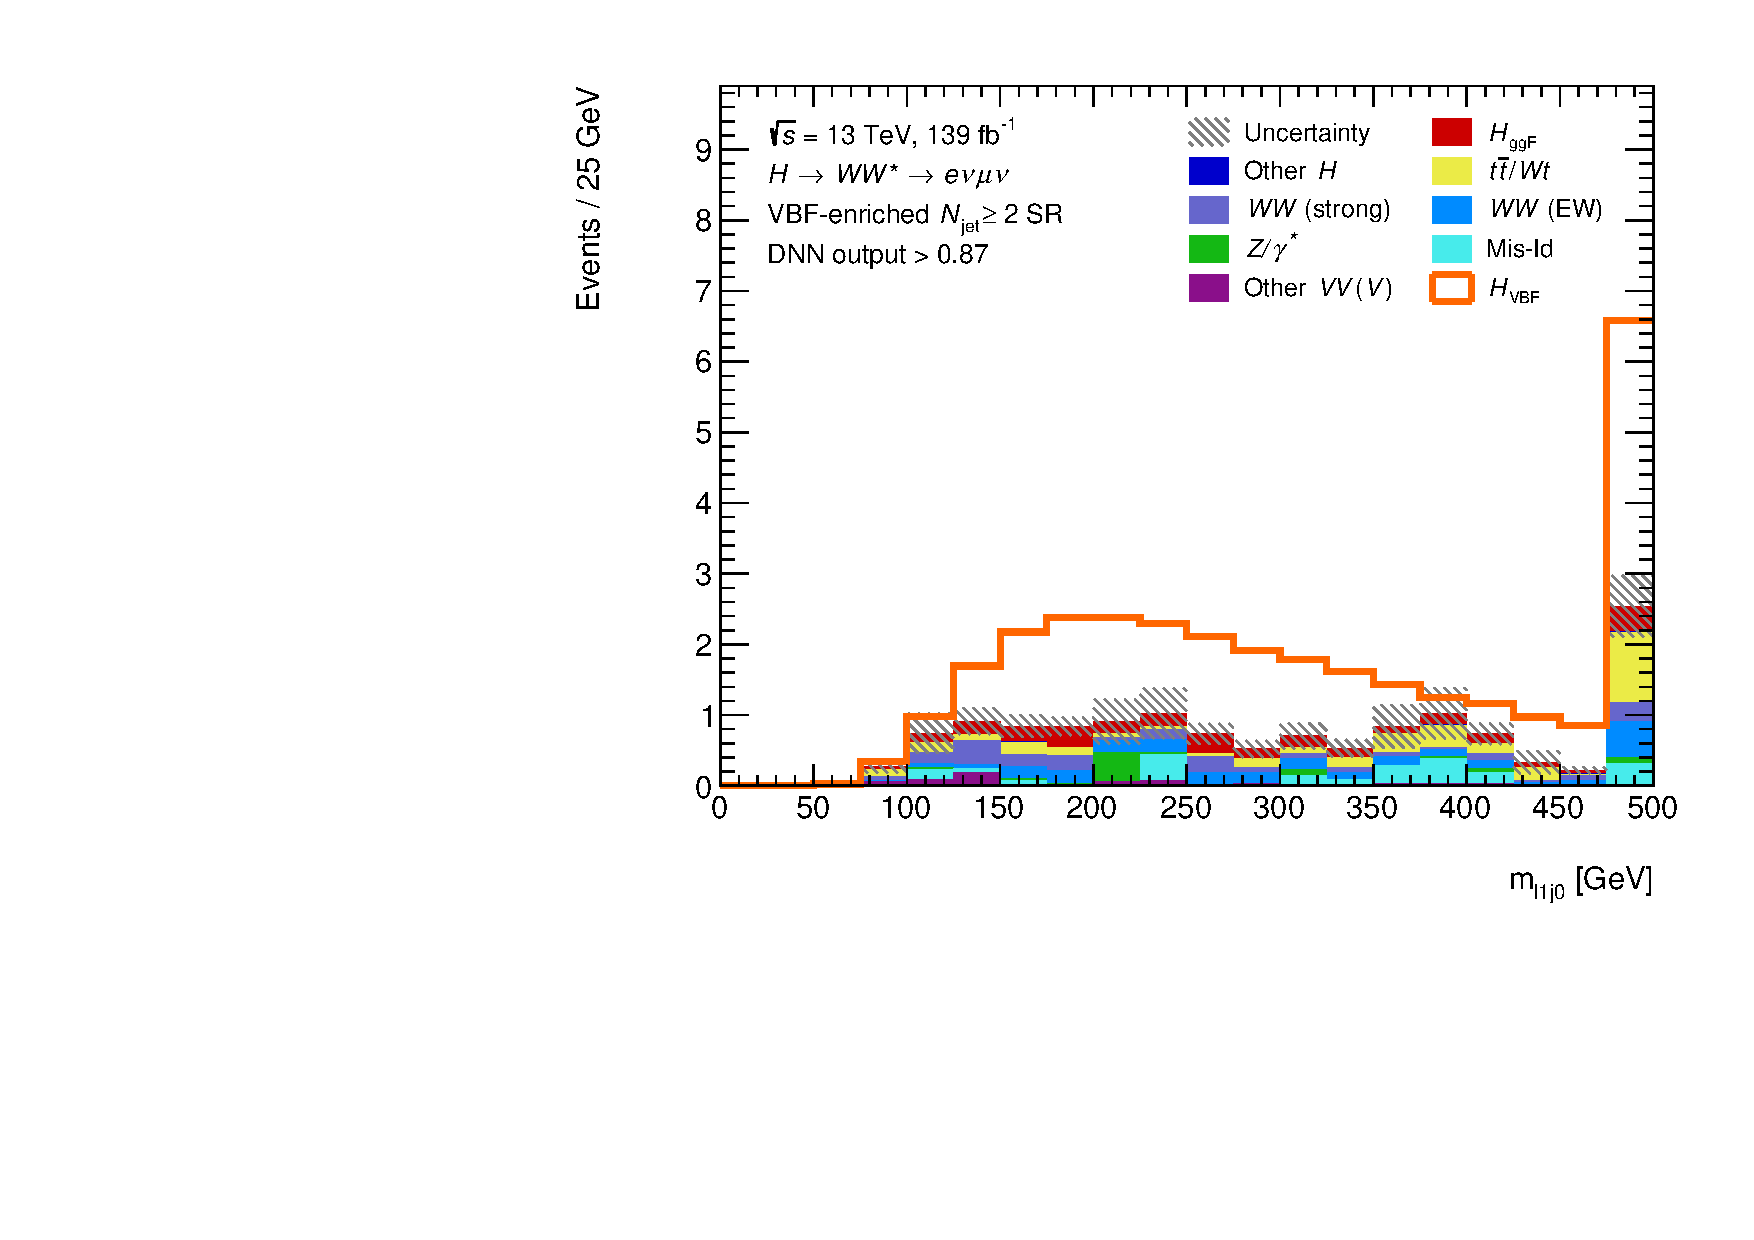
\includegraphics[width=0.32\textwidth]{figures/hww/dnn/blinded/run2-emme-CutVBFSR_DNN87-Ml1j0-lin.pdf}
    } \\
    \subfloat[$\mlonejtwo$]{
        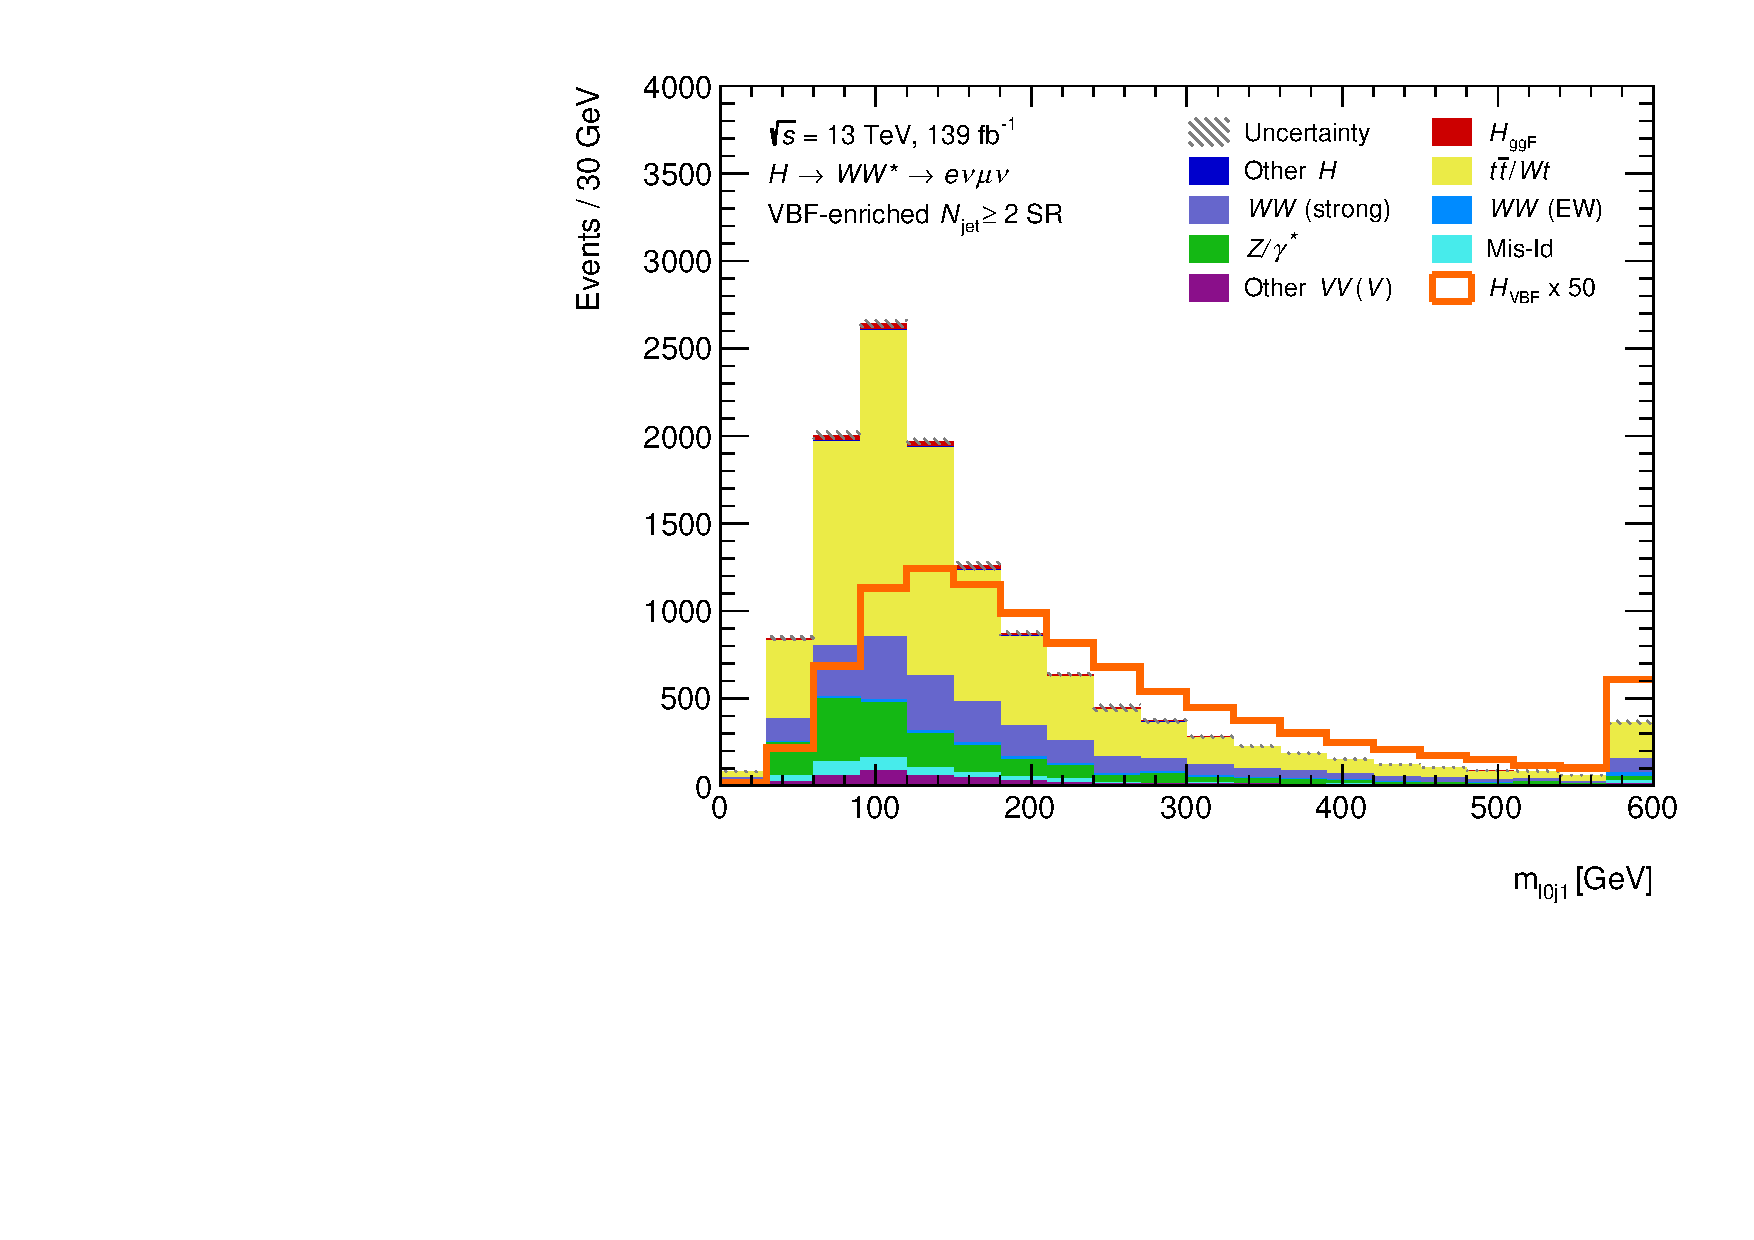
\includegraphics[width=0.32\textwidth]{figures/hww/dnn/blinded/run2-emme-CutVBF_SR-Ml0j1-lin.pdf} \hfill
        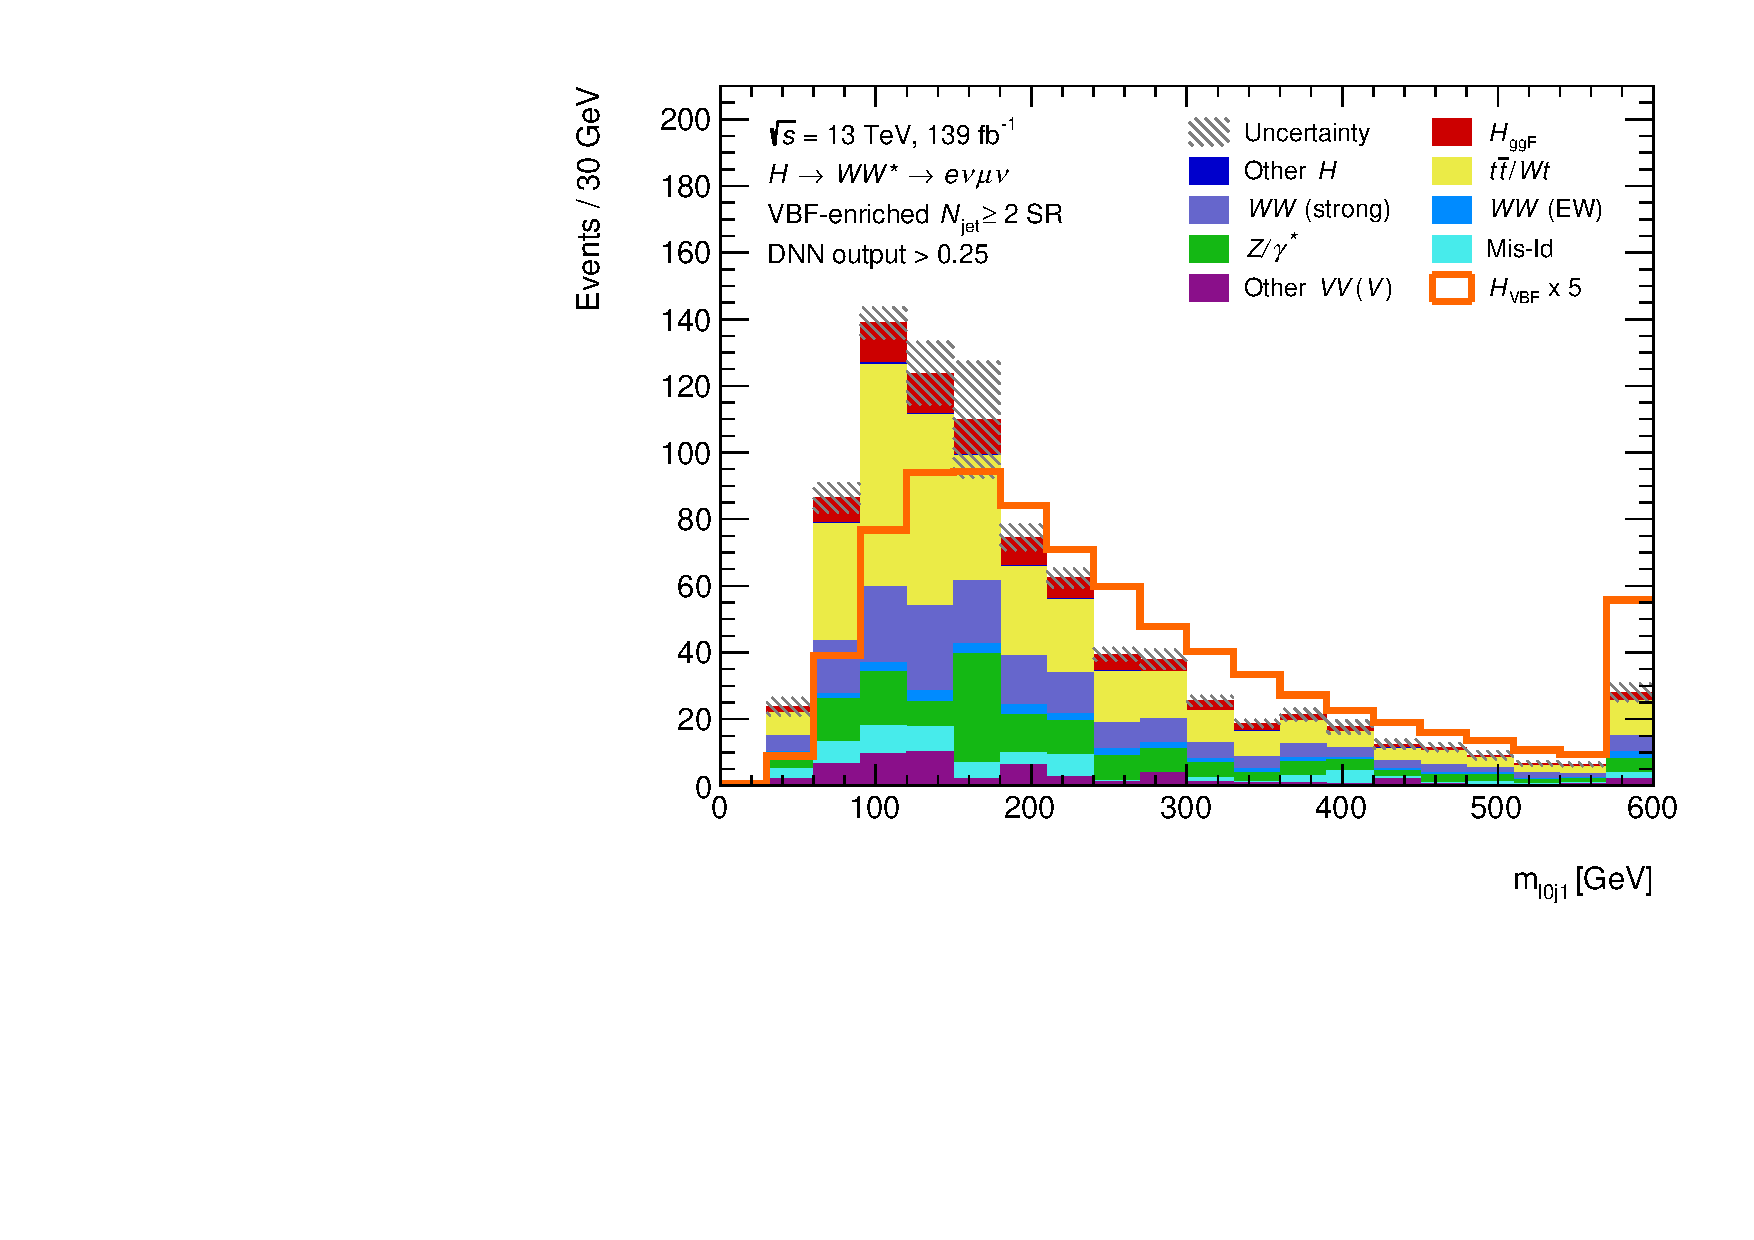
\includegraphics[width=0.32\textwidth]{figures/hww/dnn/blinded/run2-emme-CutVBFSR_DNN25-Ml0j1-lin.pdf} \hfill
        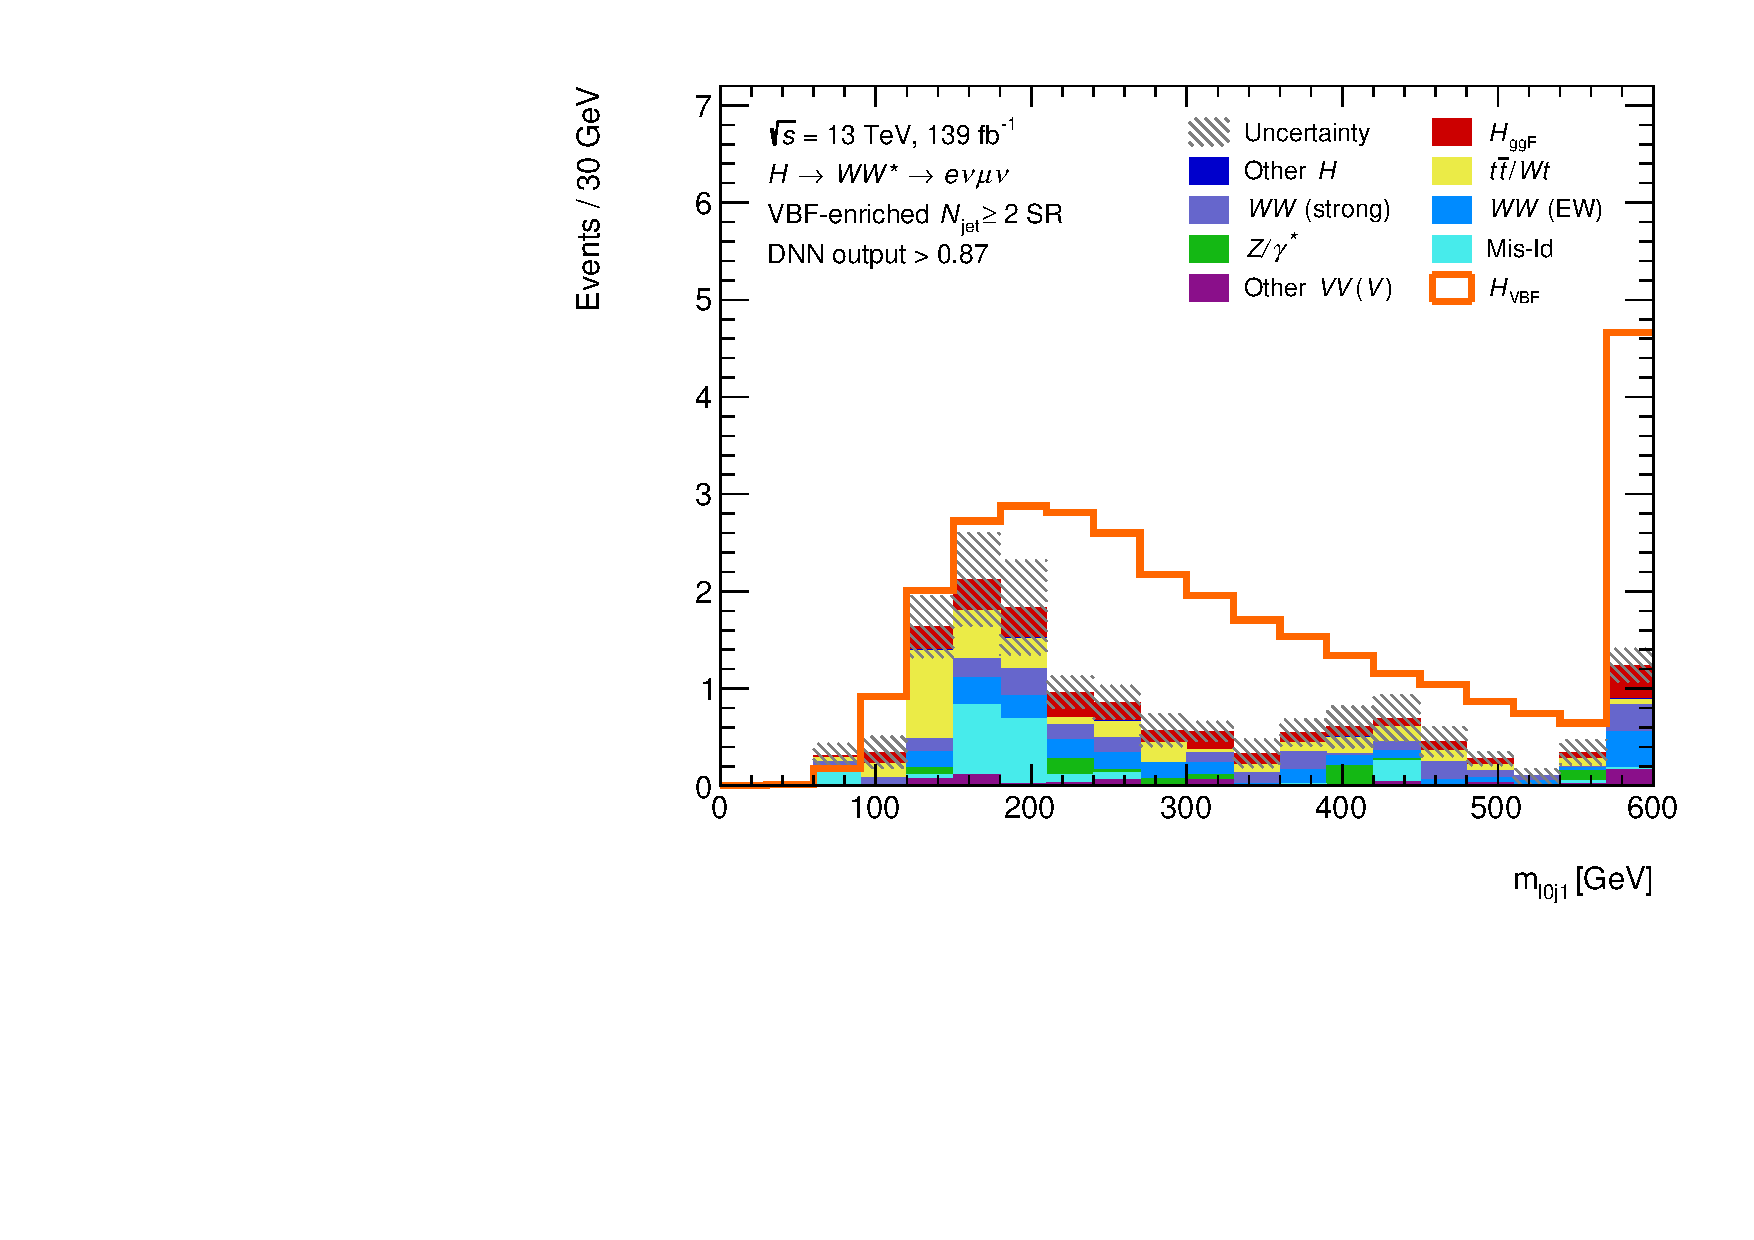
\includegraphics[width=0.32\textwidth]{figures/hww/dnn/blinded/run2-emme-CutVBFSR_DNN87-Ml0j1-lin.pdf}
    } \\
    \subfloat[$\mltwojtwo$]{
        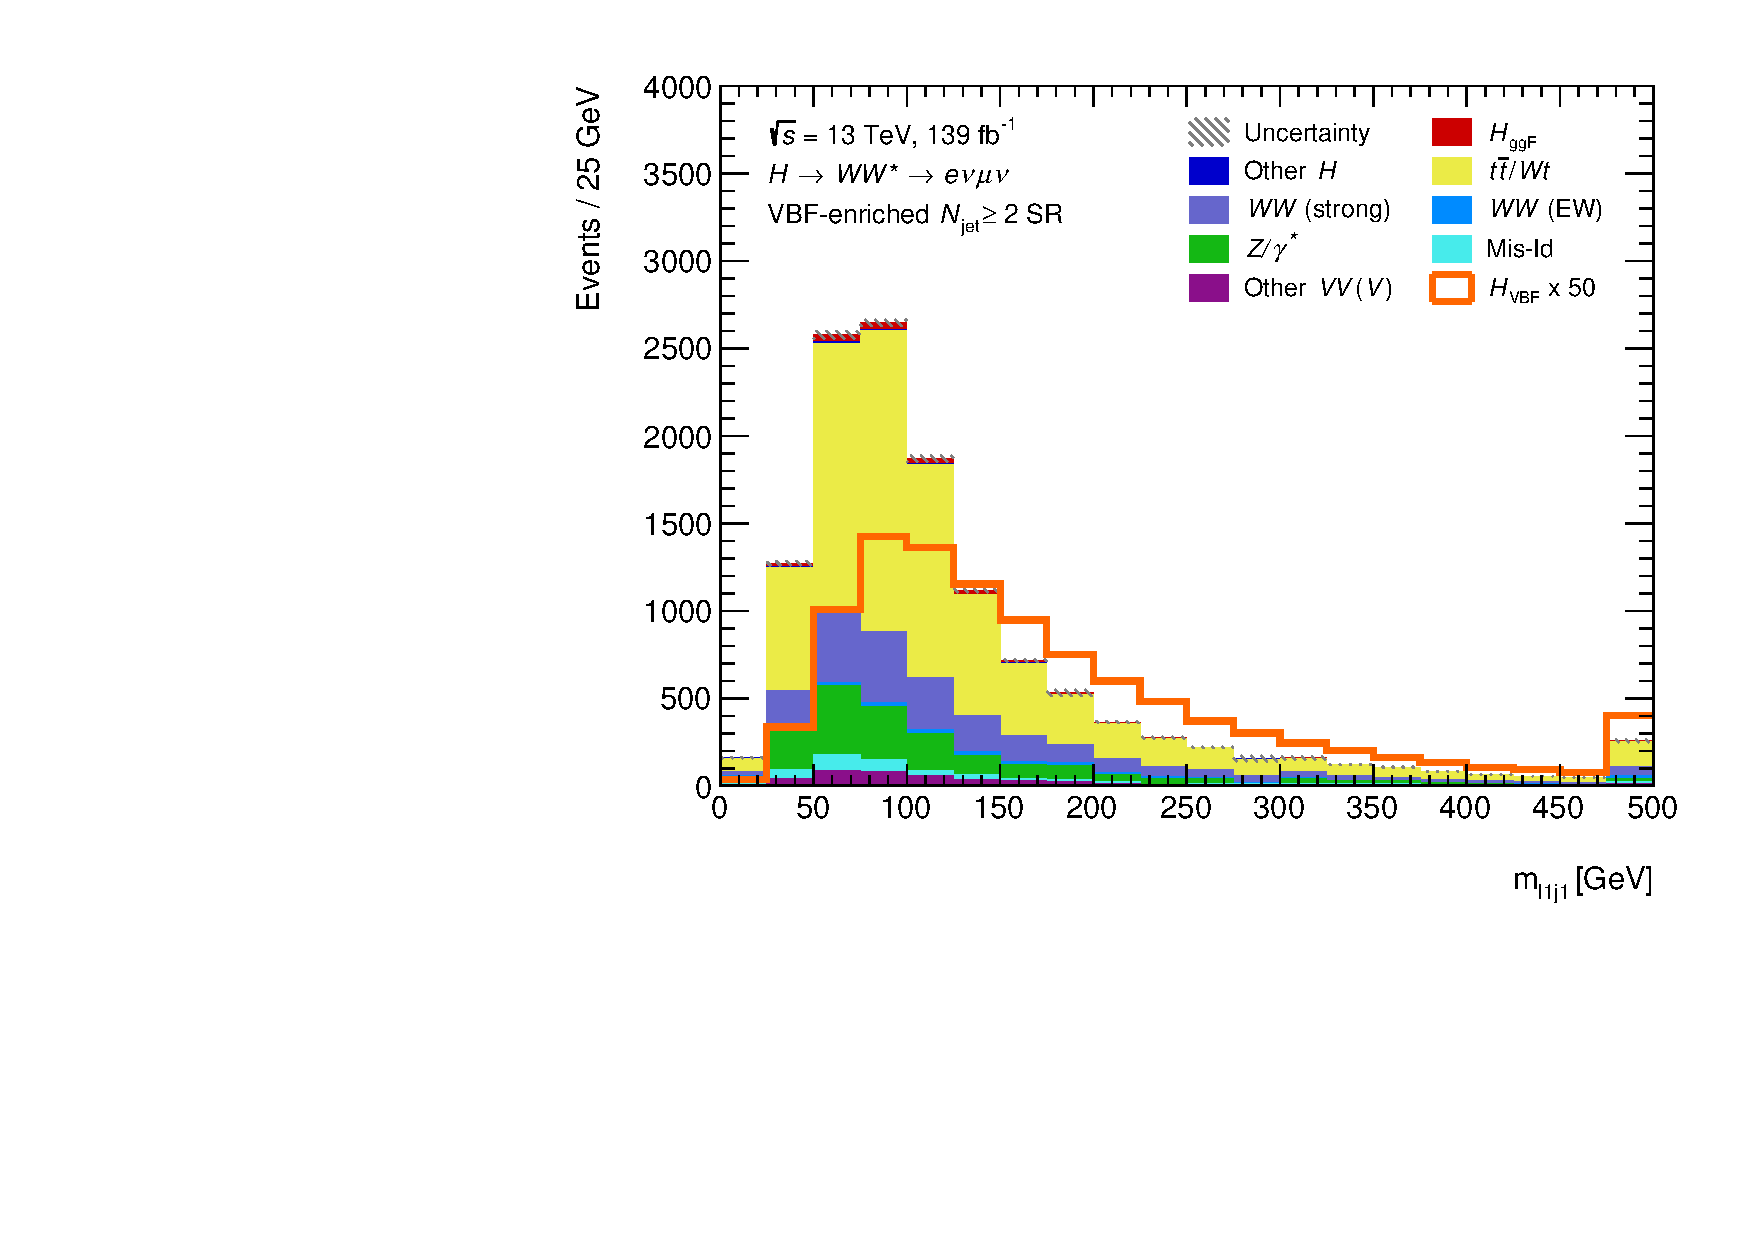
\includegraphics[width=0.32\textwidth]{figures/hww/dnn/blinded/run2-emme-CutVBF_SR-Ml1j1-lin.pdf} \hfill
        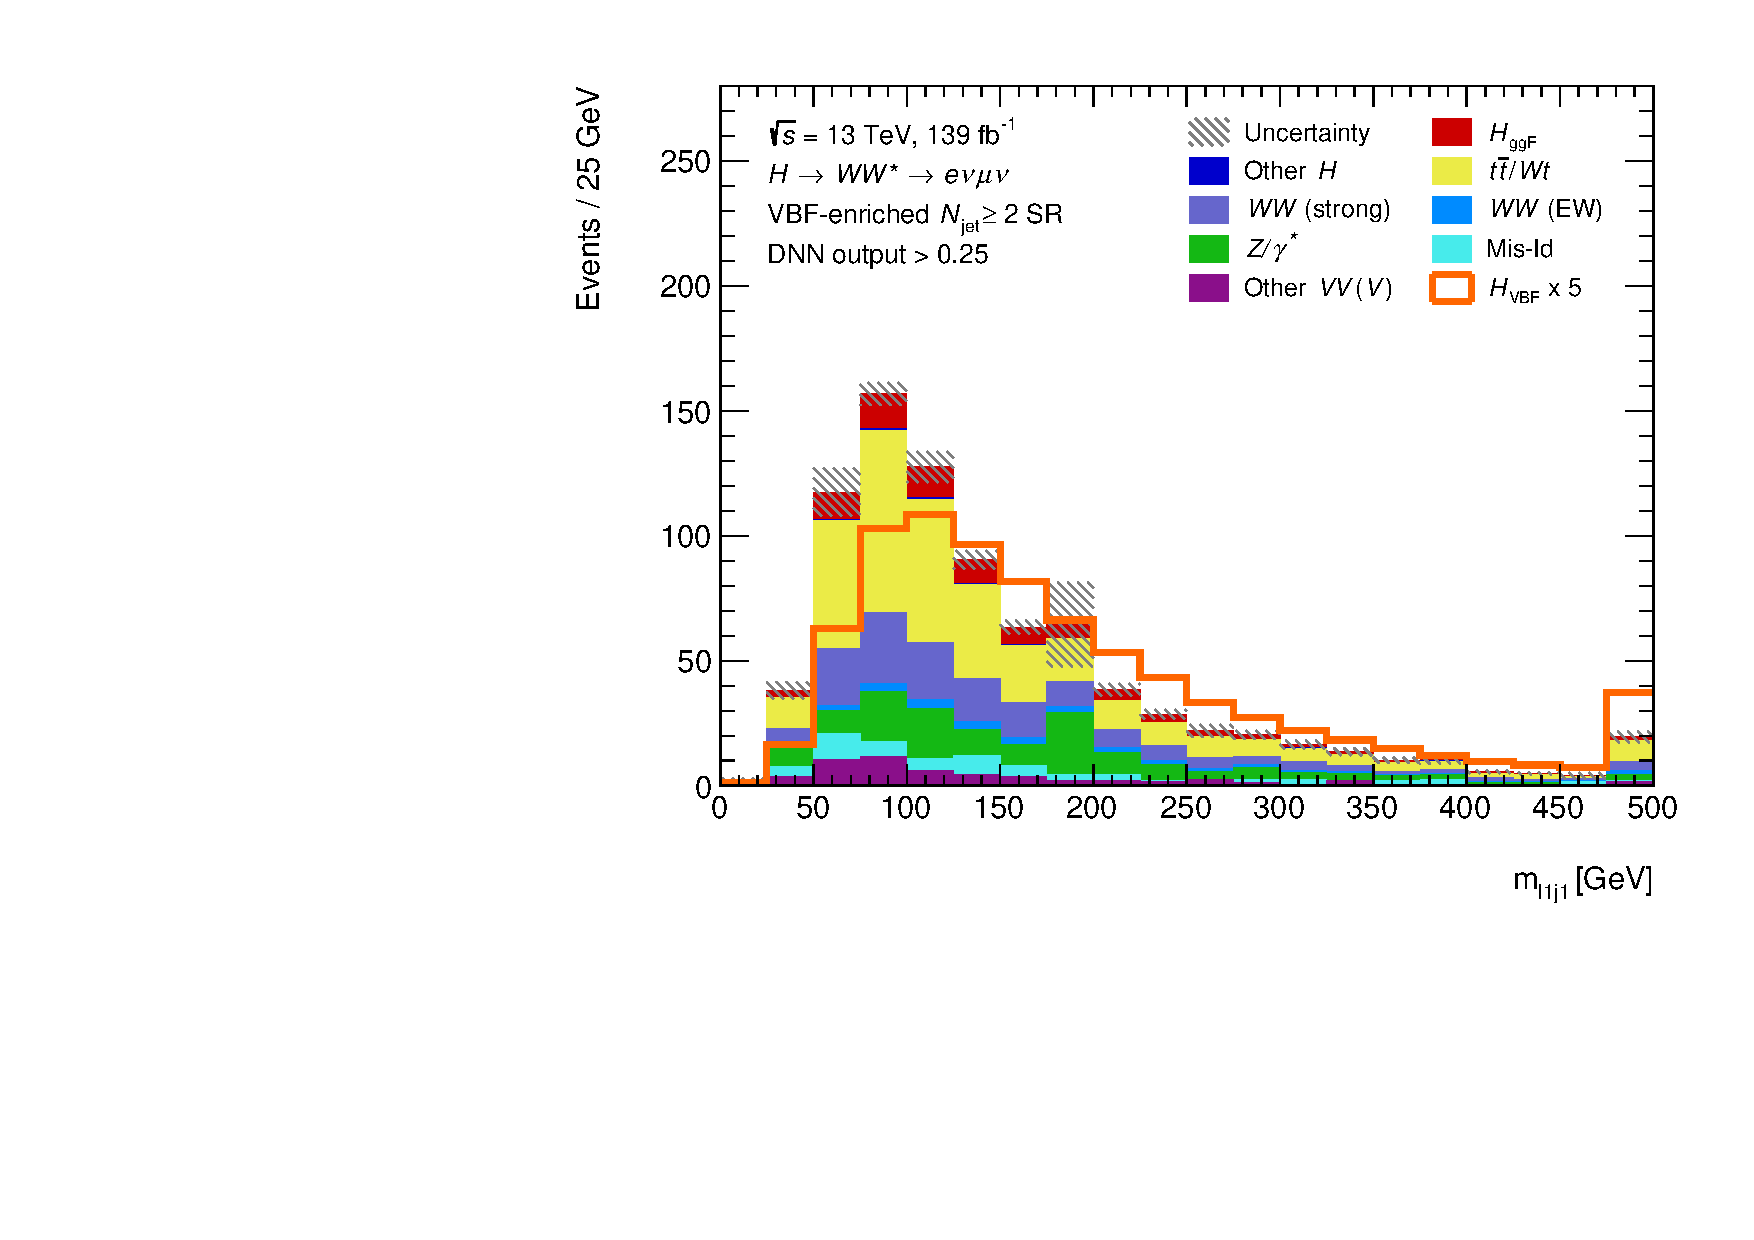
\includegraphics[width=0.32\textwidth]{figures/hww/dnn/blinded/run2-emme-CutVBFSR_DNN25-Ml1j1-lin.pdf} \hfill
        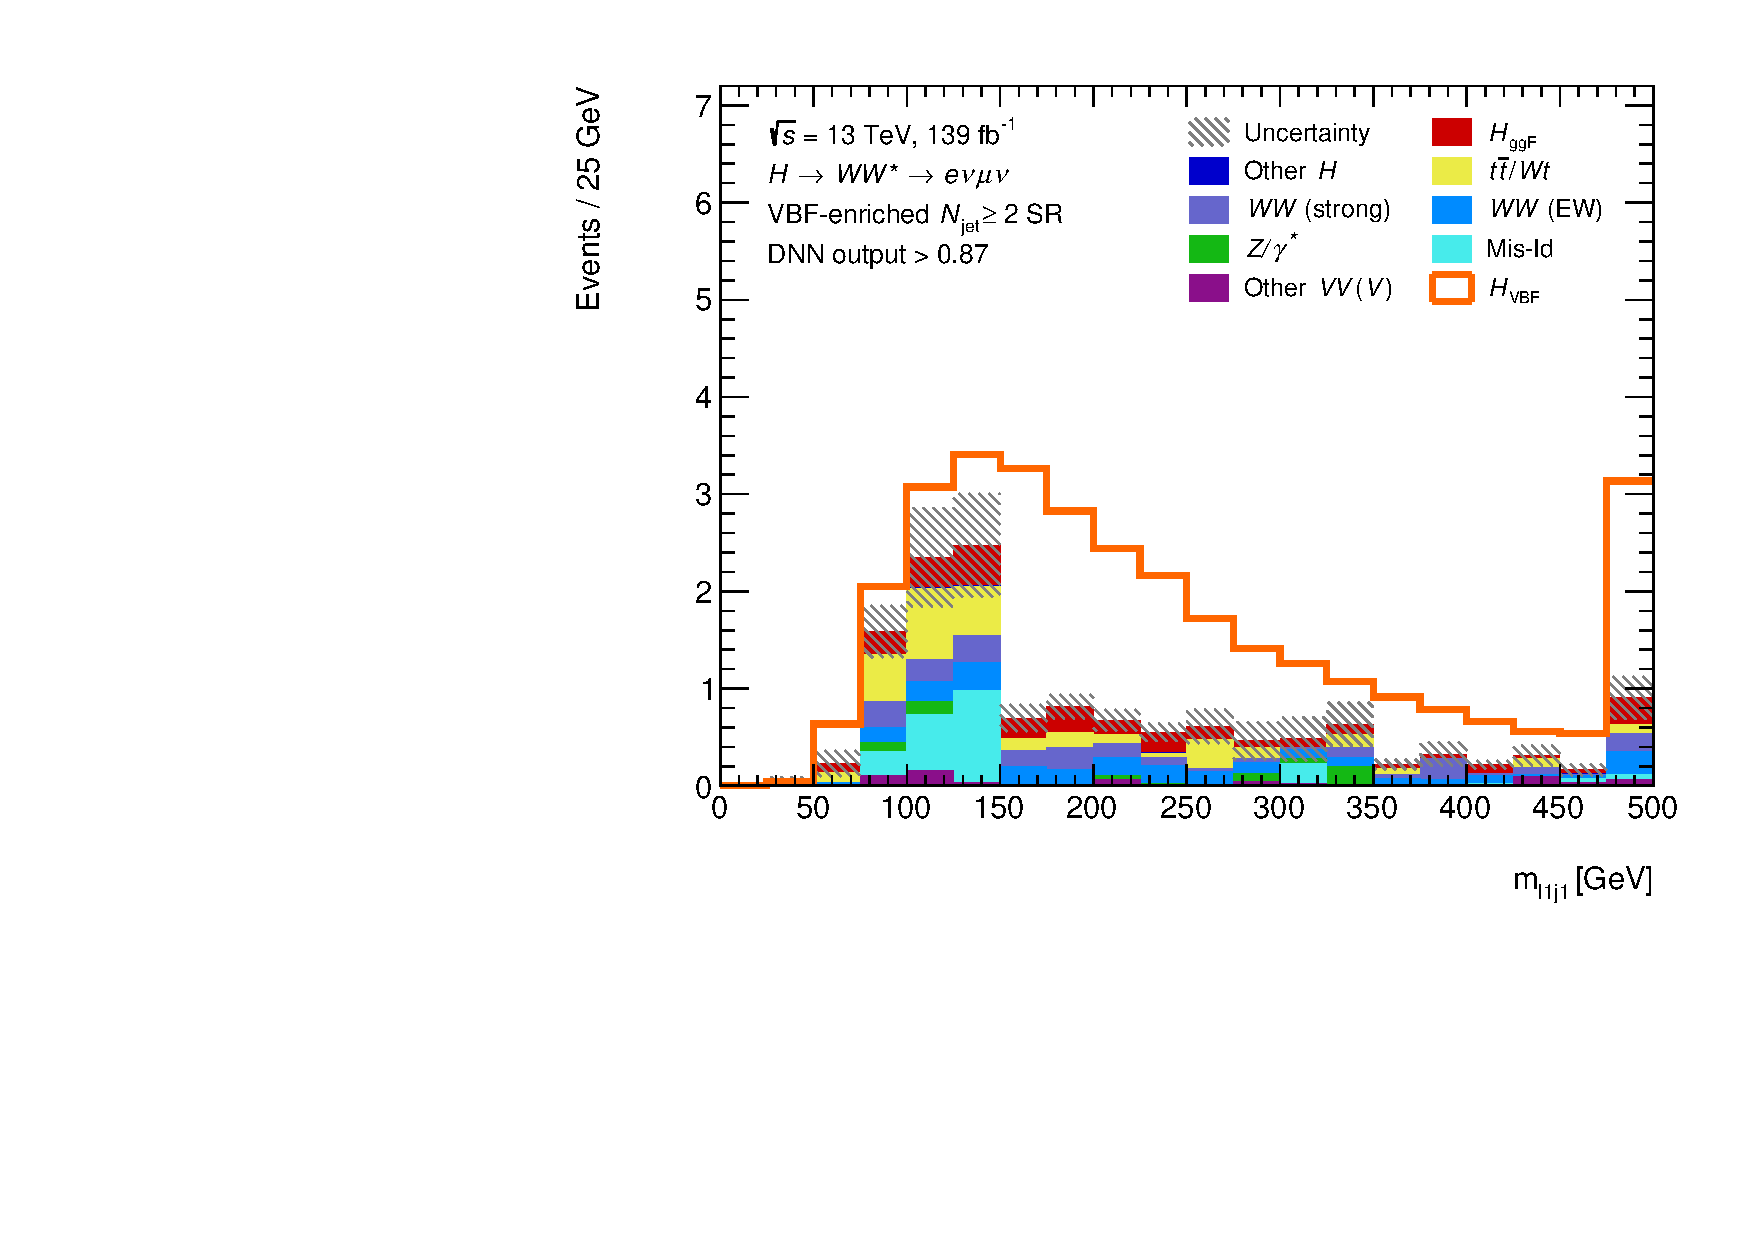
\includegraphics[width=0.32\textwidth]{figures/hww/dnn/blinded/run2-emme-CutVBFSR_DNN87-Ml1j1-lin.pdf}
    } 
    {\caption{Distributions of $\mlonejone$, $\mltwojone$, $\mlonejtwo$, and $\mltwojtwo$ in the VBF signal region.
            Each row shows one variable with different cuts on the DNN output distribution being applied in different columns.
            \label{app:fig:dnn-inputs-vbf-top2} }}
\end{figure}


\begin{figure}[h]
    \centering
    \subfloat[$\pTjone$]{
        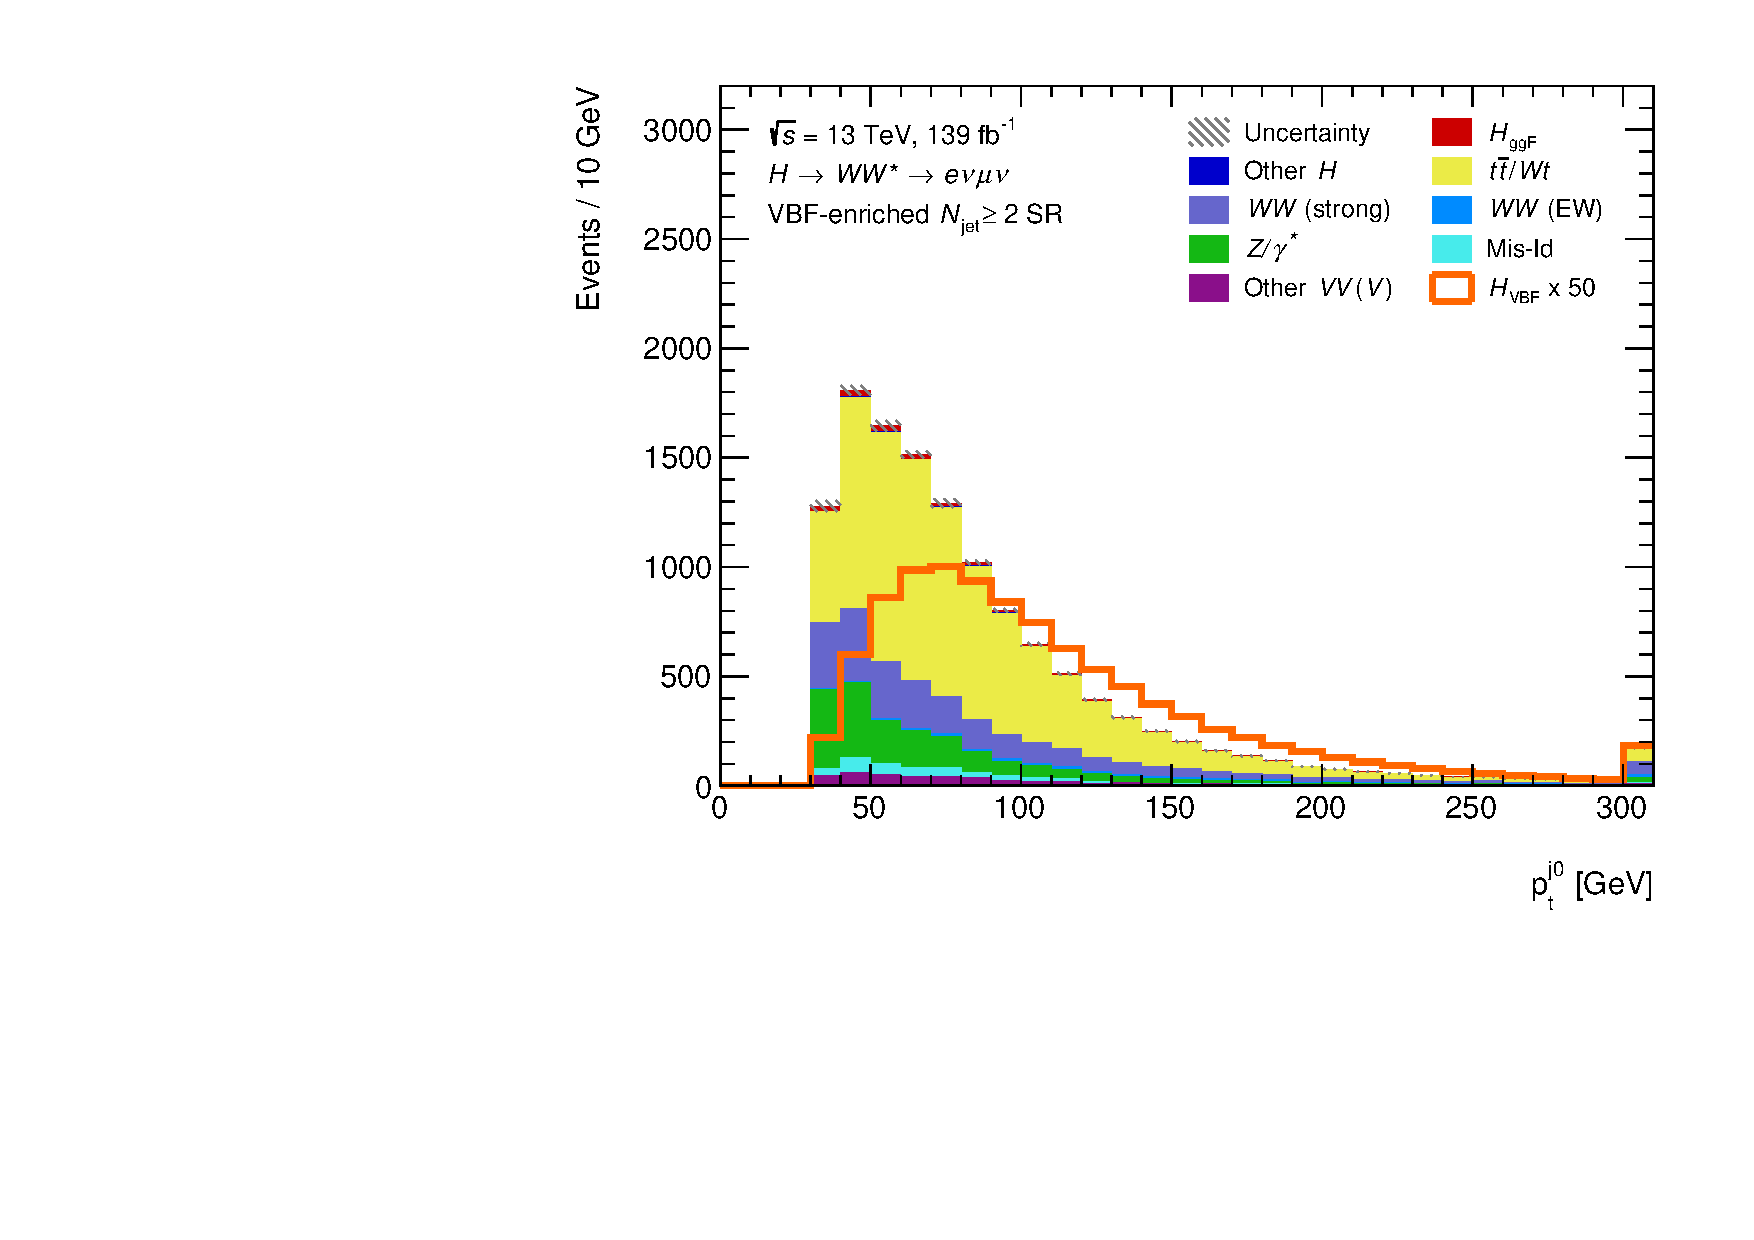
\includegraphics[width=0.32\textwidth]{figures/hww/dnn/blinded/run2-emme-CutVBF_SR-leadJetPt-lin.pdf} \hfill
        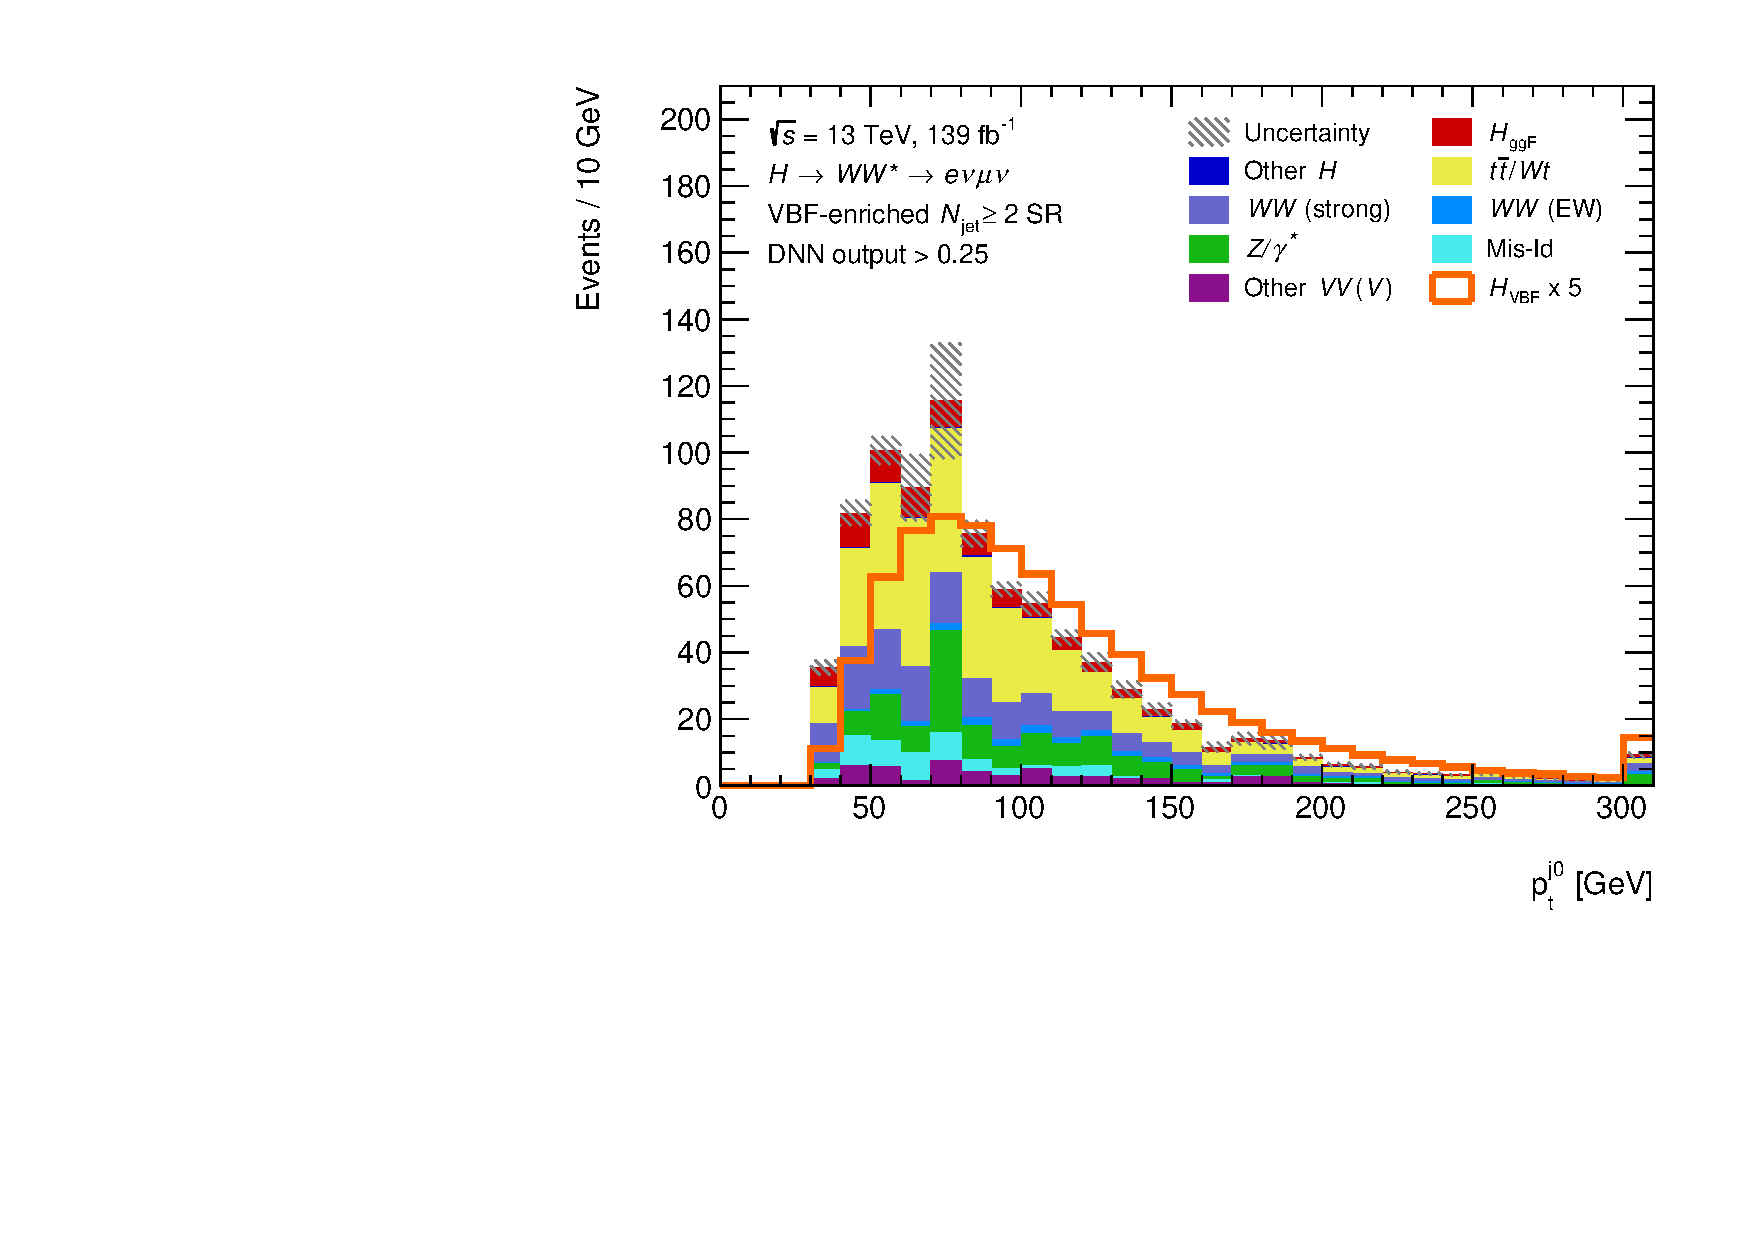
\includegraphics[width=0.32\textwidth]{figures/hww/dnn/blinded/run2-emme-CutVBFSR_DNN25-leadJetPt-lin.pdf} \hfill
        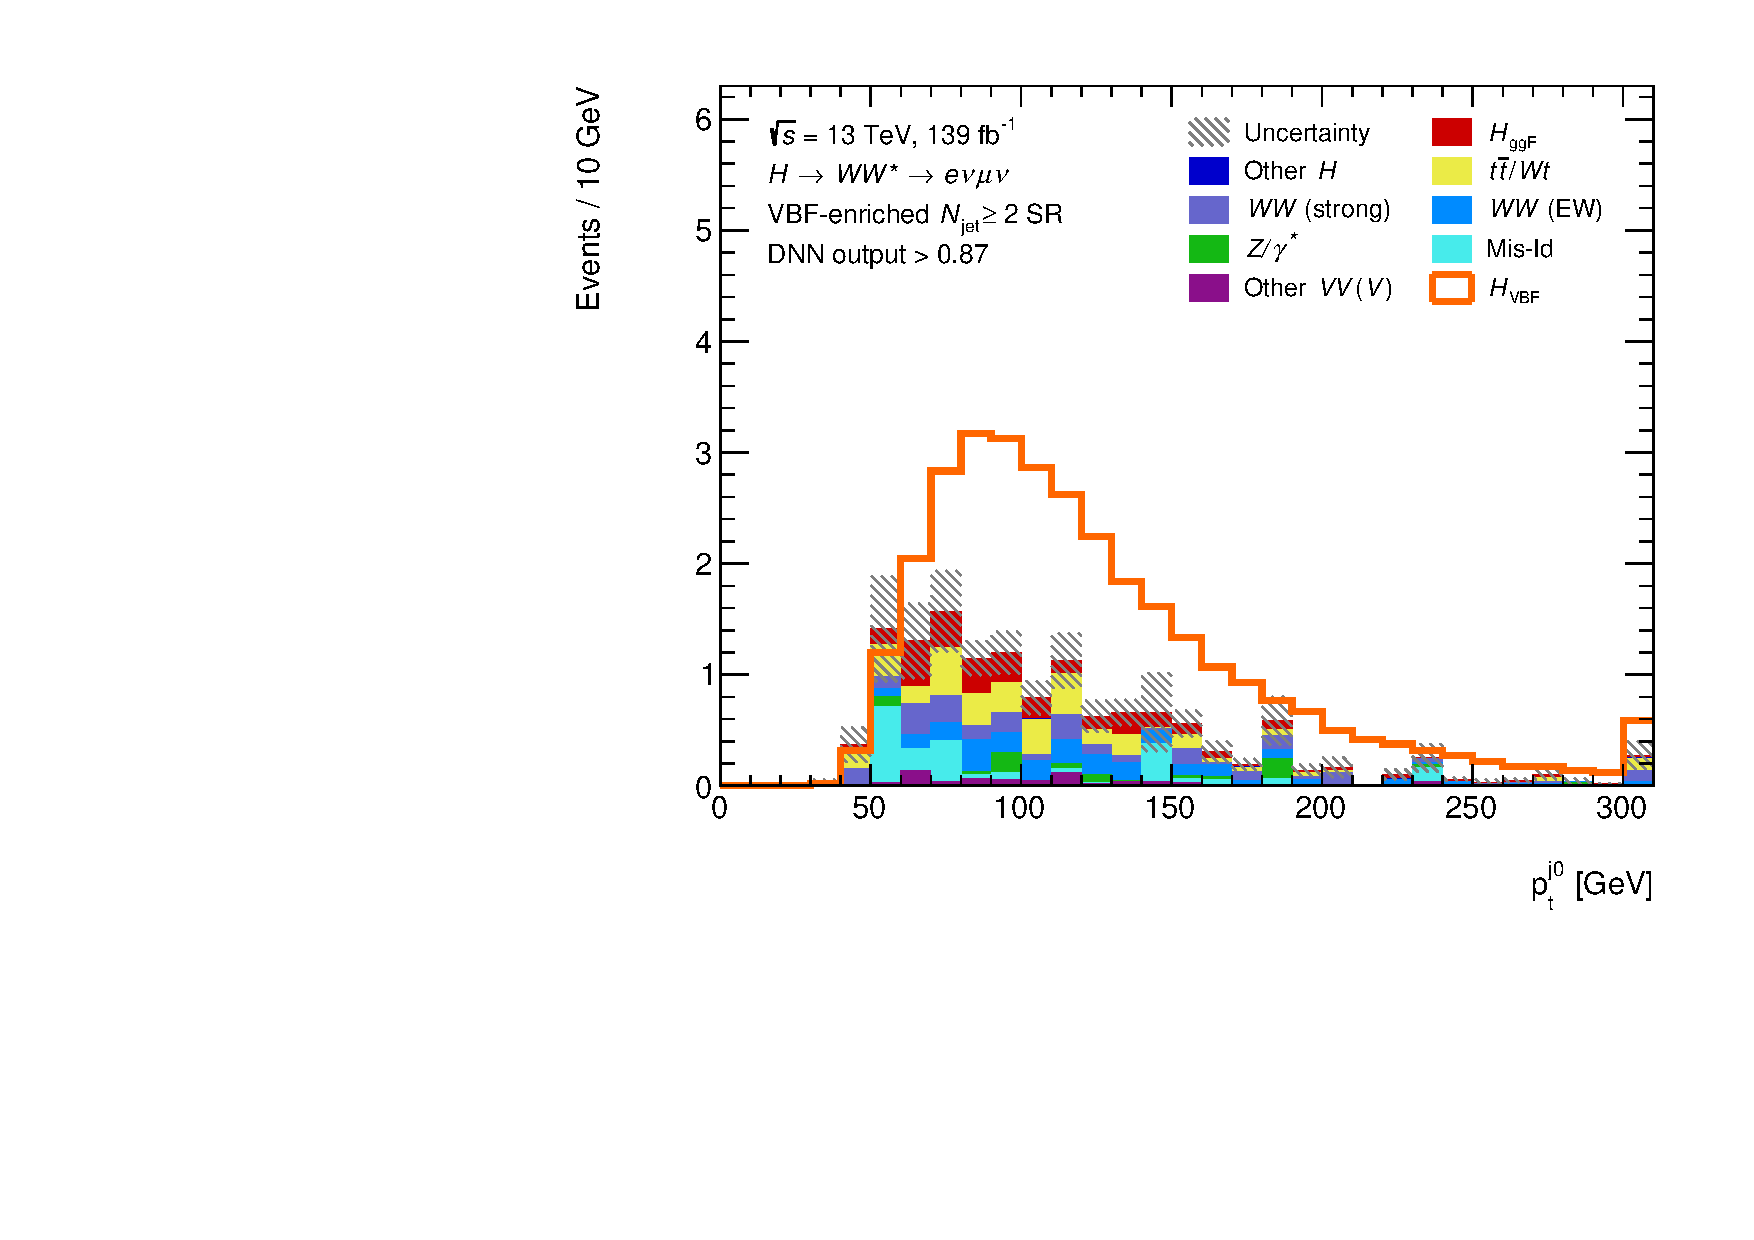
\includegraphics[width=0.32\textwidth]{figures/hww/dnn/blinded/run2-emme-CutVBFSR_DNN87-leadJetPt-lin.pdf}
    } \\
    \subfloat[$\pTjtwo$]{
        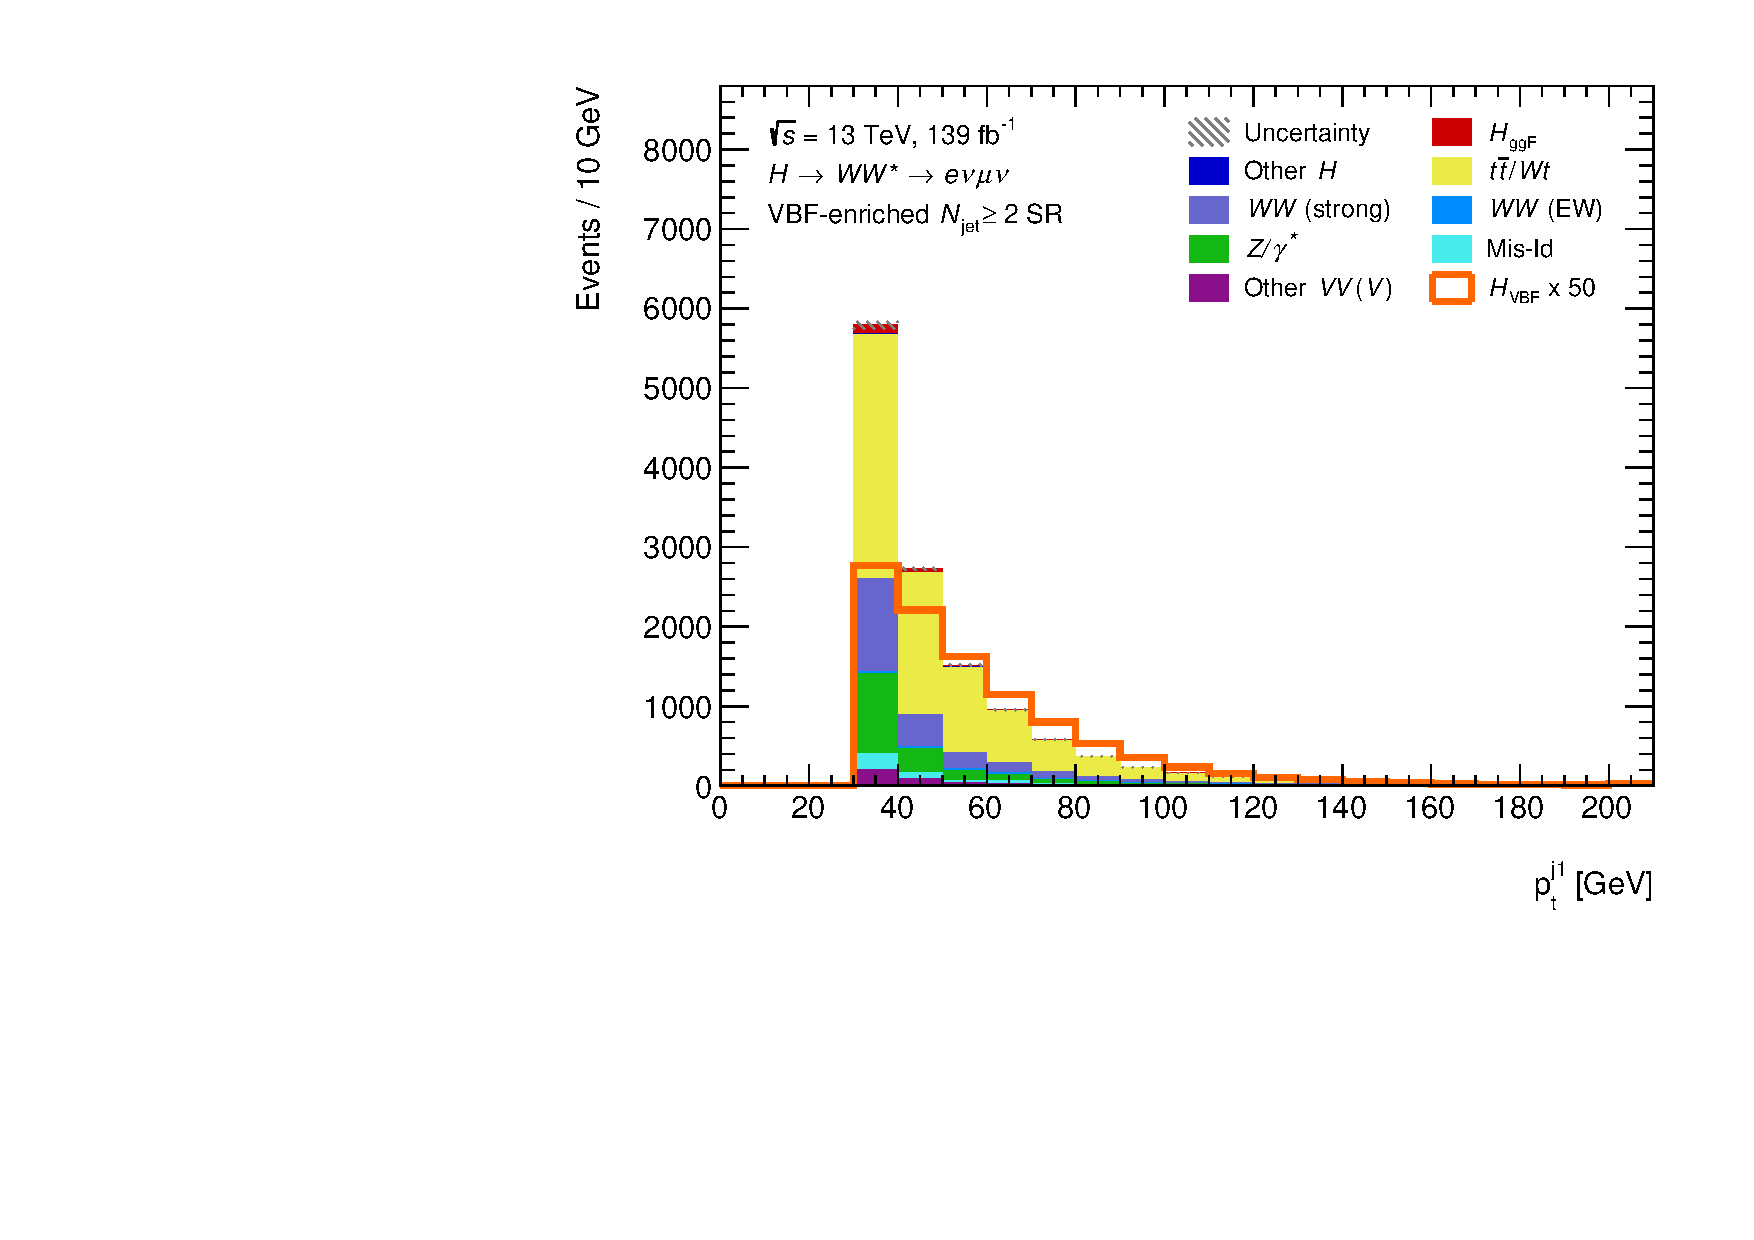
\includegraphics[width=0.32\textwidth]{figures/hww/dnn/blinded/run2-emme-CutVBF_SR-subleadJetPt-lin.pdf} \hfill
        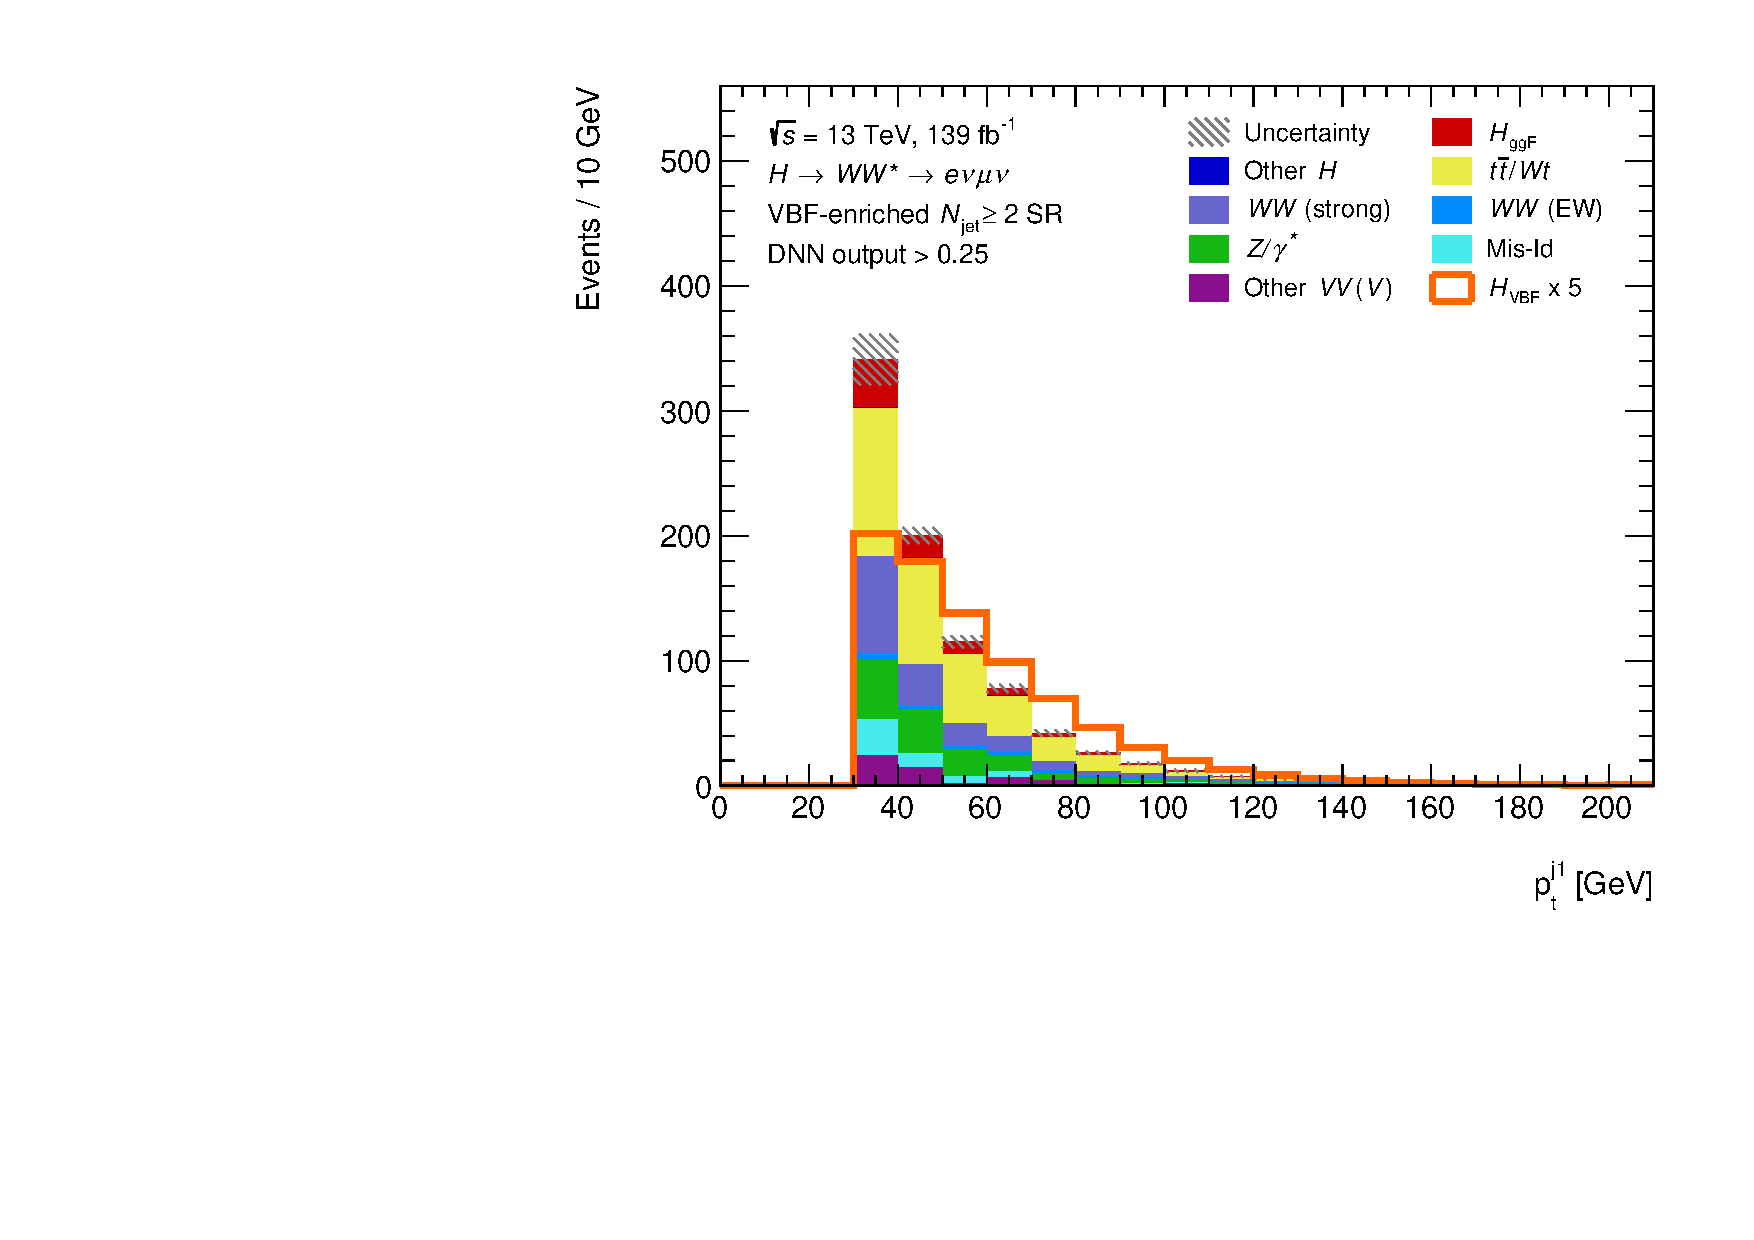
\includegraphics[width=0.32\textwidth]{figures/hww/dnn/blinded/run2-emme-CutVBFSR_DNN25-subleadJetPt-lin.pdf} \hfill
        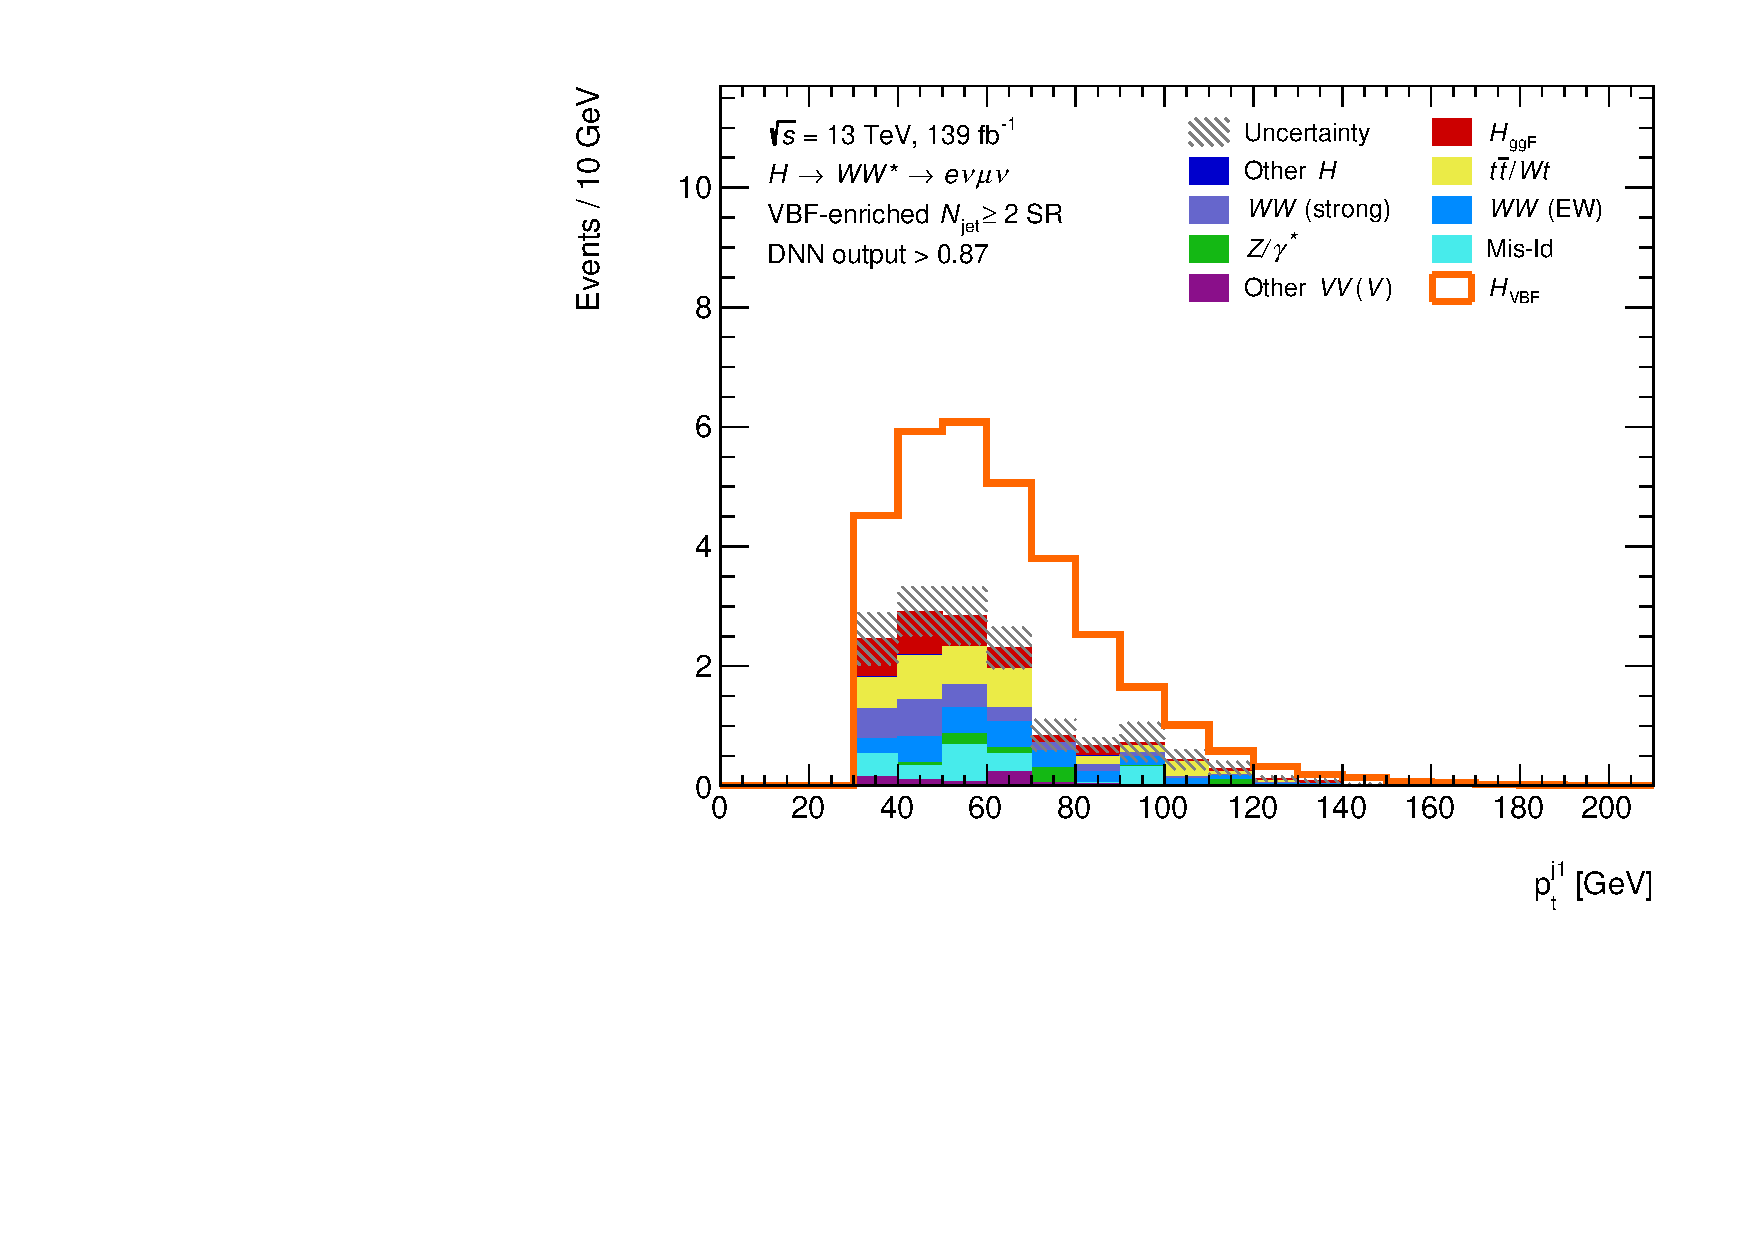
\includegraphics[width=0.32\textwidth]{figures/hww/dnn/blinded/run2-emme-CutVBFSR_DNN87-subleadJetPt-lin.pdf}
    } \\
    \subfloat[$\pTjthree$]{
        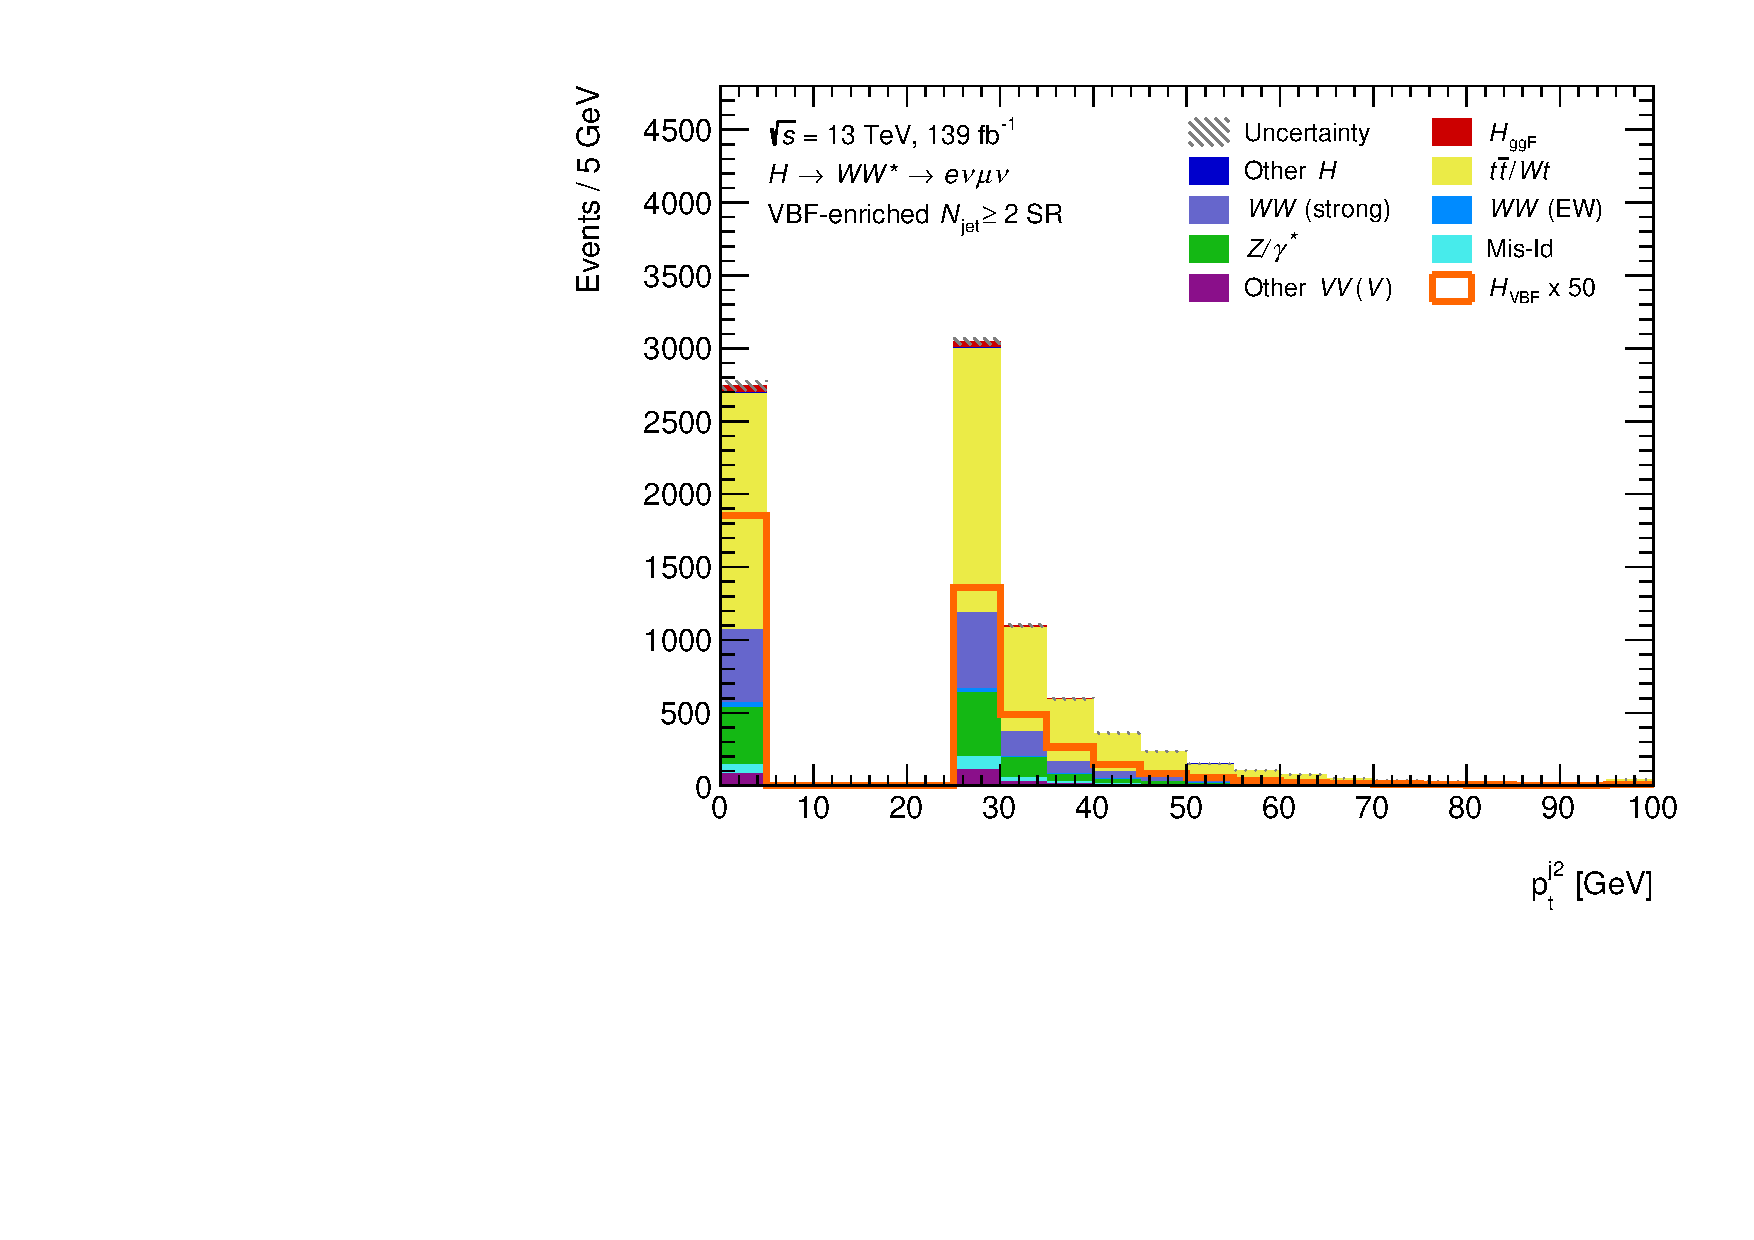
\includegraphics[width=0.32\textwidth]{figures/hww/dnn/blinded/run2-emme-CutVBF_SR-thirdJetPt-lin.pdf} \hfill
        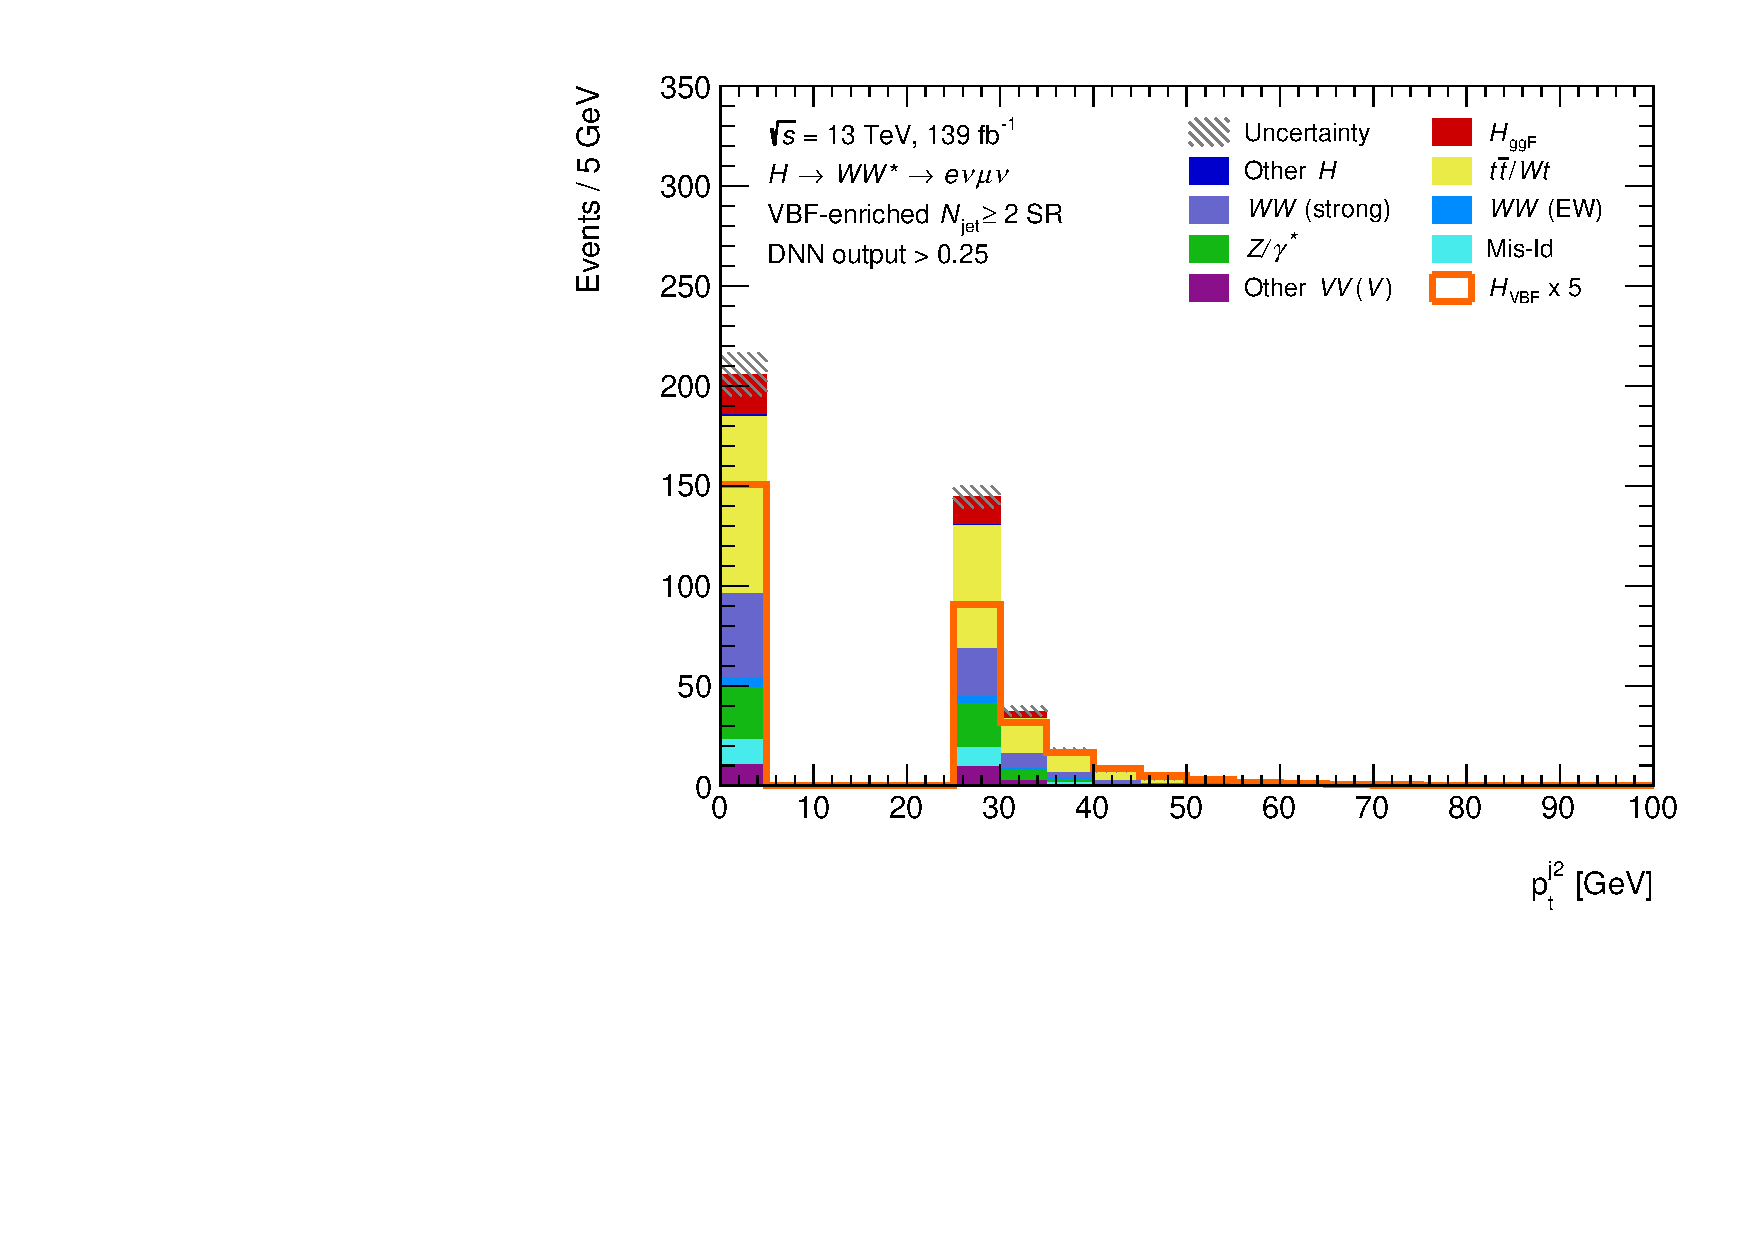
\includegraphics[width=0.32\textwidth]{figures/hww/dnn/blinded/run2-emme-CutVBFSR_DNN25-thirdJetPt-lin.pdf} \hfill
        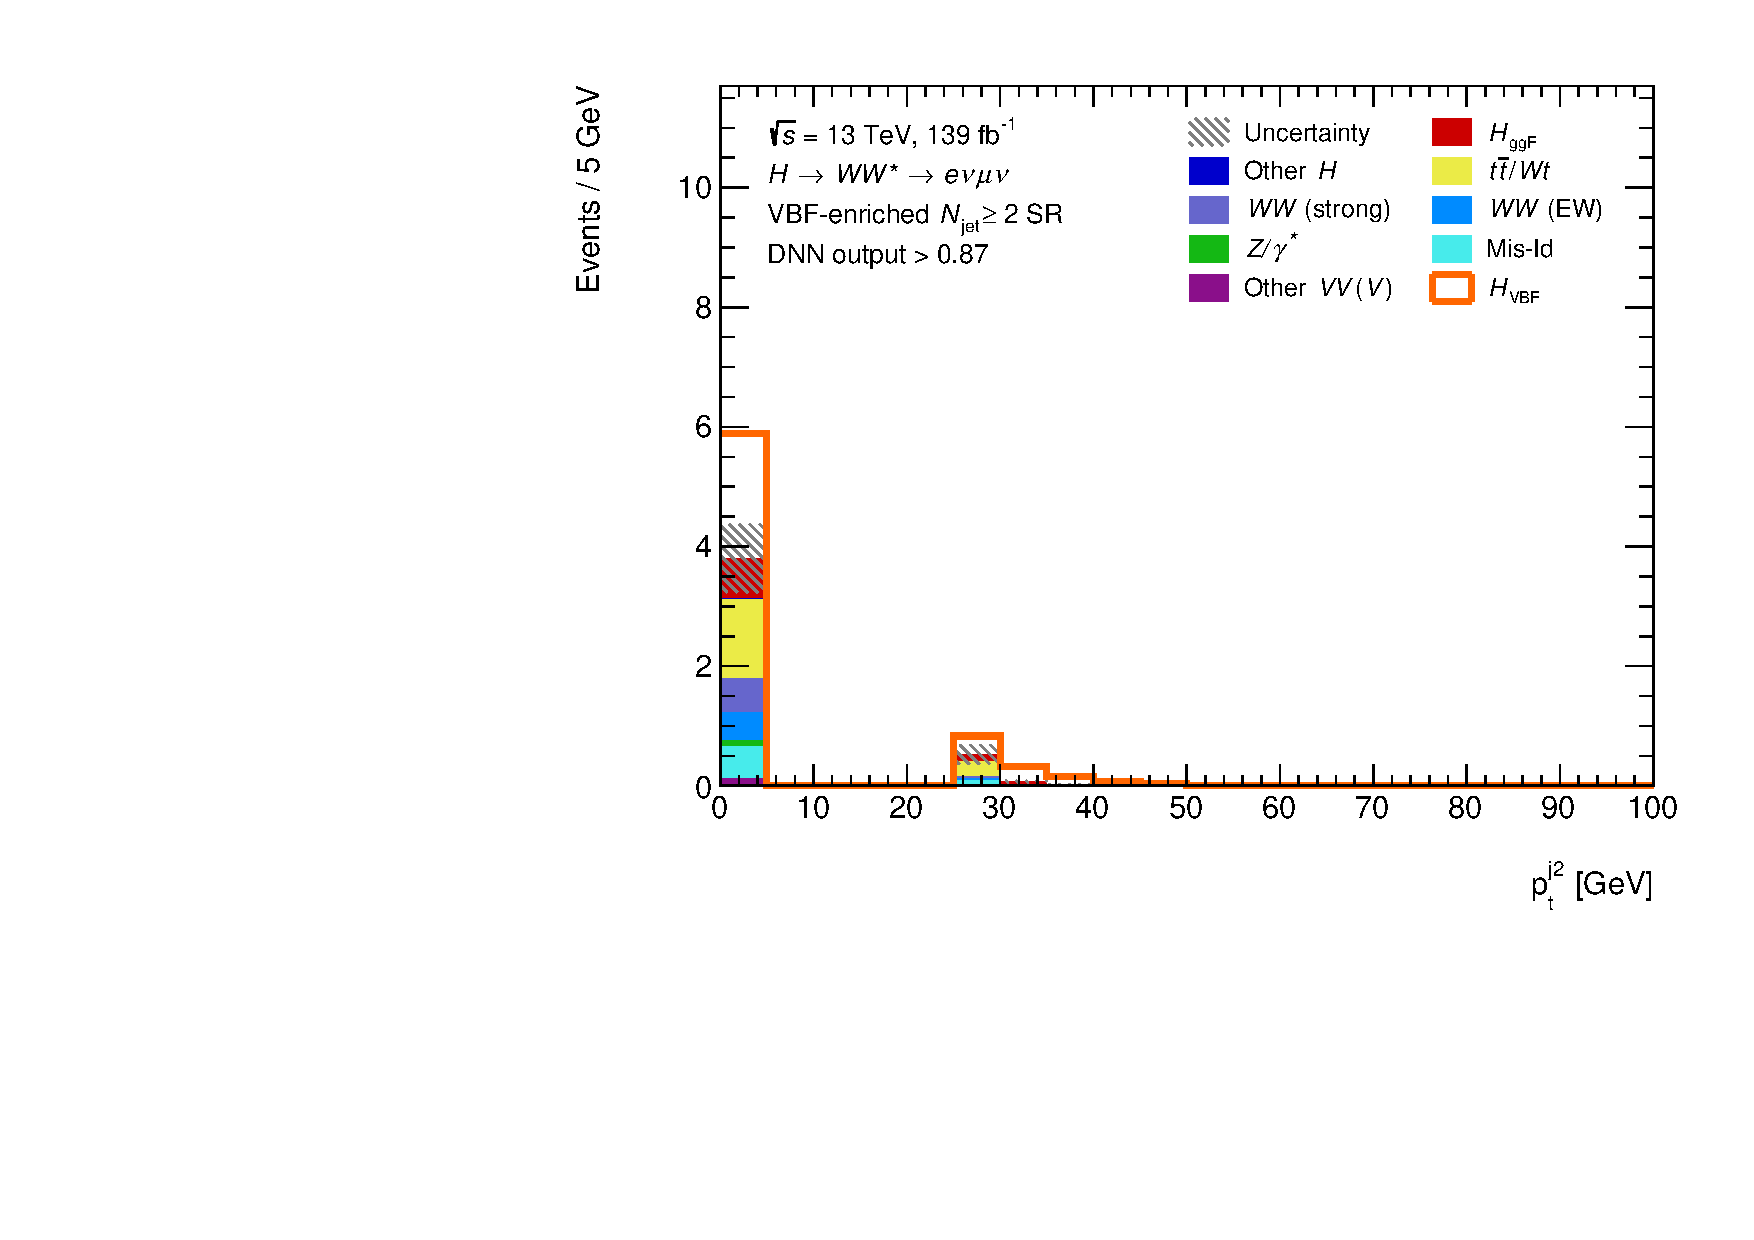
\includegraphics[width=0.32\textwidth]{figures/hww/dnn/blinded/run2-emme-CutVBFSR_DNN87-thirdJetPt-lin.pdf}
    } 
    {\caption{Distributions of $\pTjone$, $\pTjtwo$, and $\pTjthree$ in the VBF signal region.
            Each row shows one variable with different cuts on the DNN output distribution being applied in different columns.
            \label{app:fig:dnn-inputs-vbf-top2} }}
\end{figure}


\begin{figure}[h]
    \centering
    \subfloat[$\dphill$]{
        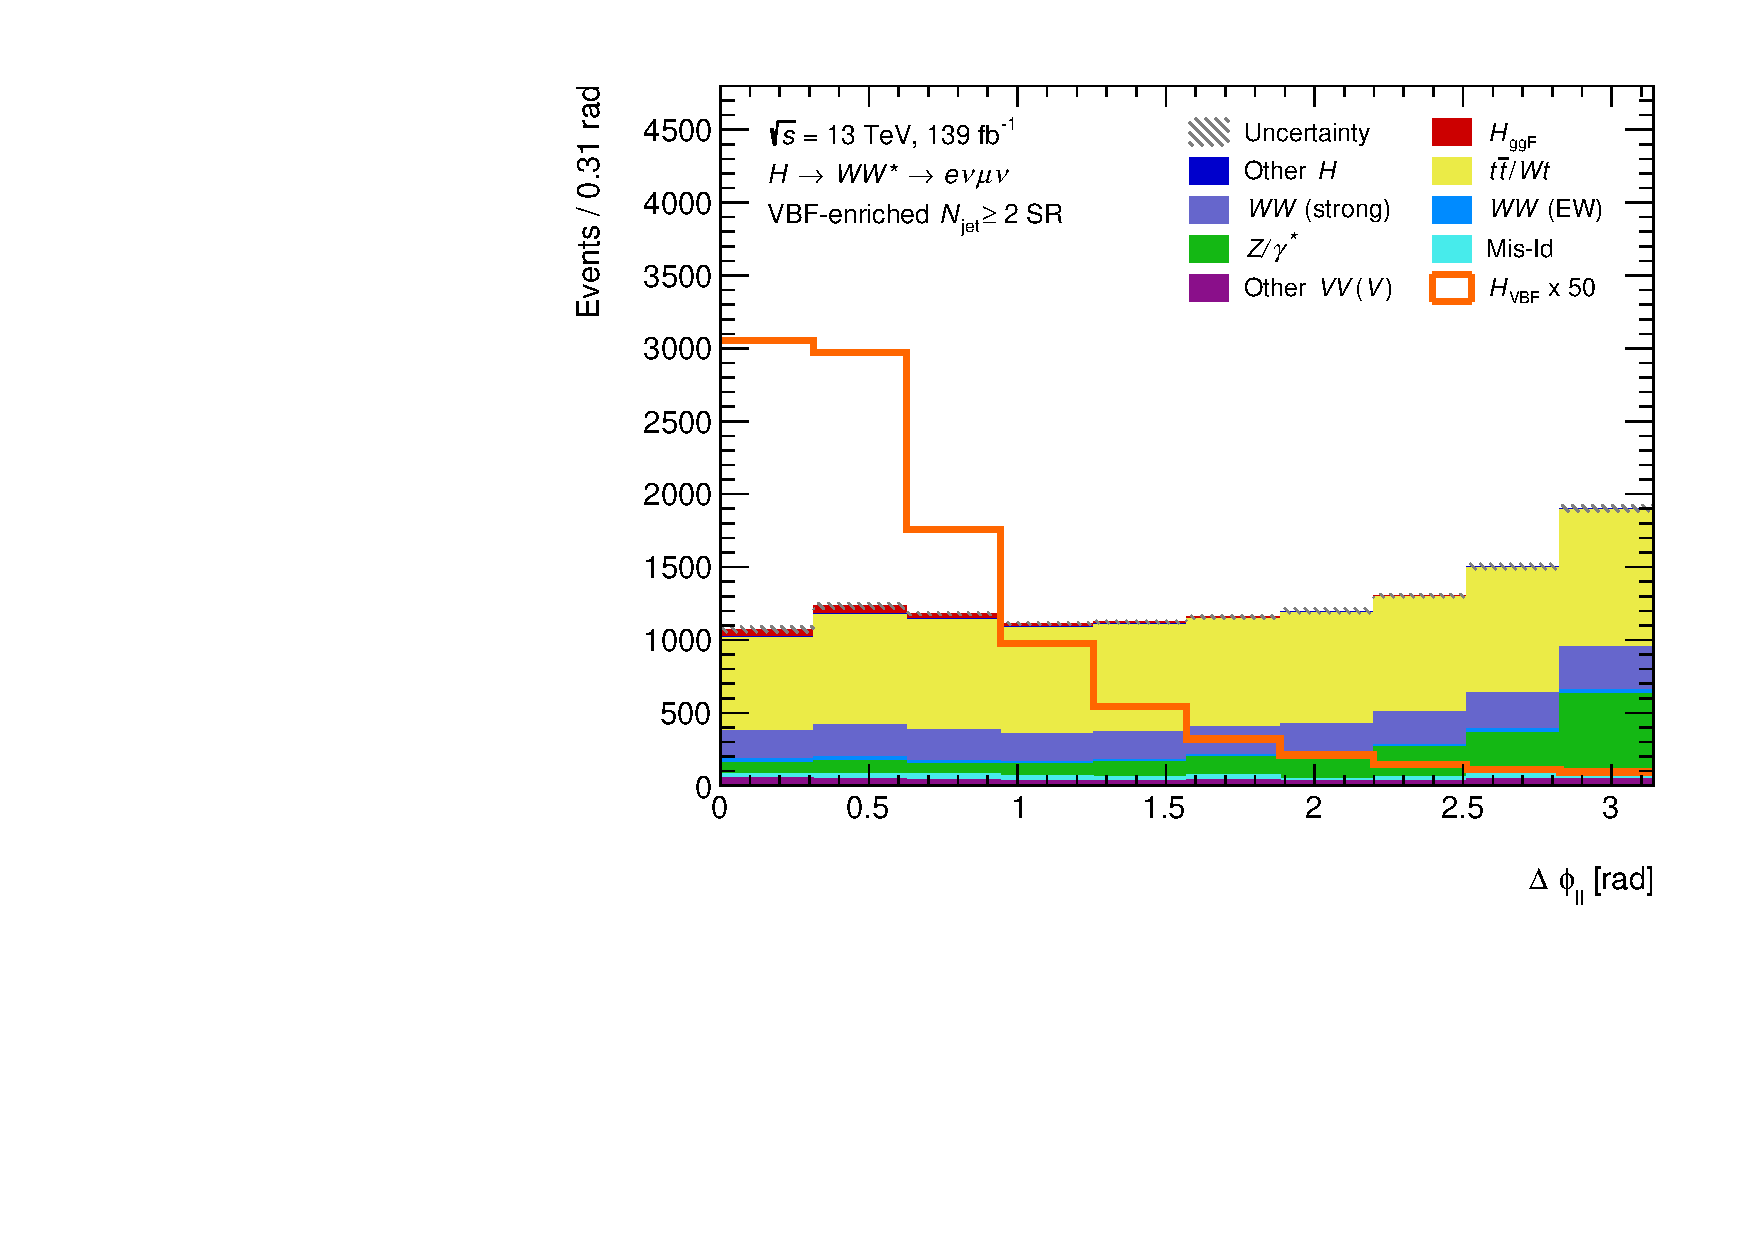
\includegraphics[width=0.32\textwidth]{figures/hww/dnn/blinded/run2-emme-CutVBF_SR-DPhill-lin.pdf} \hfill
        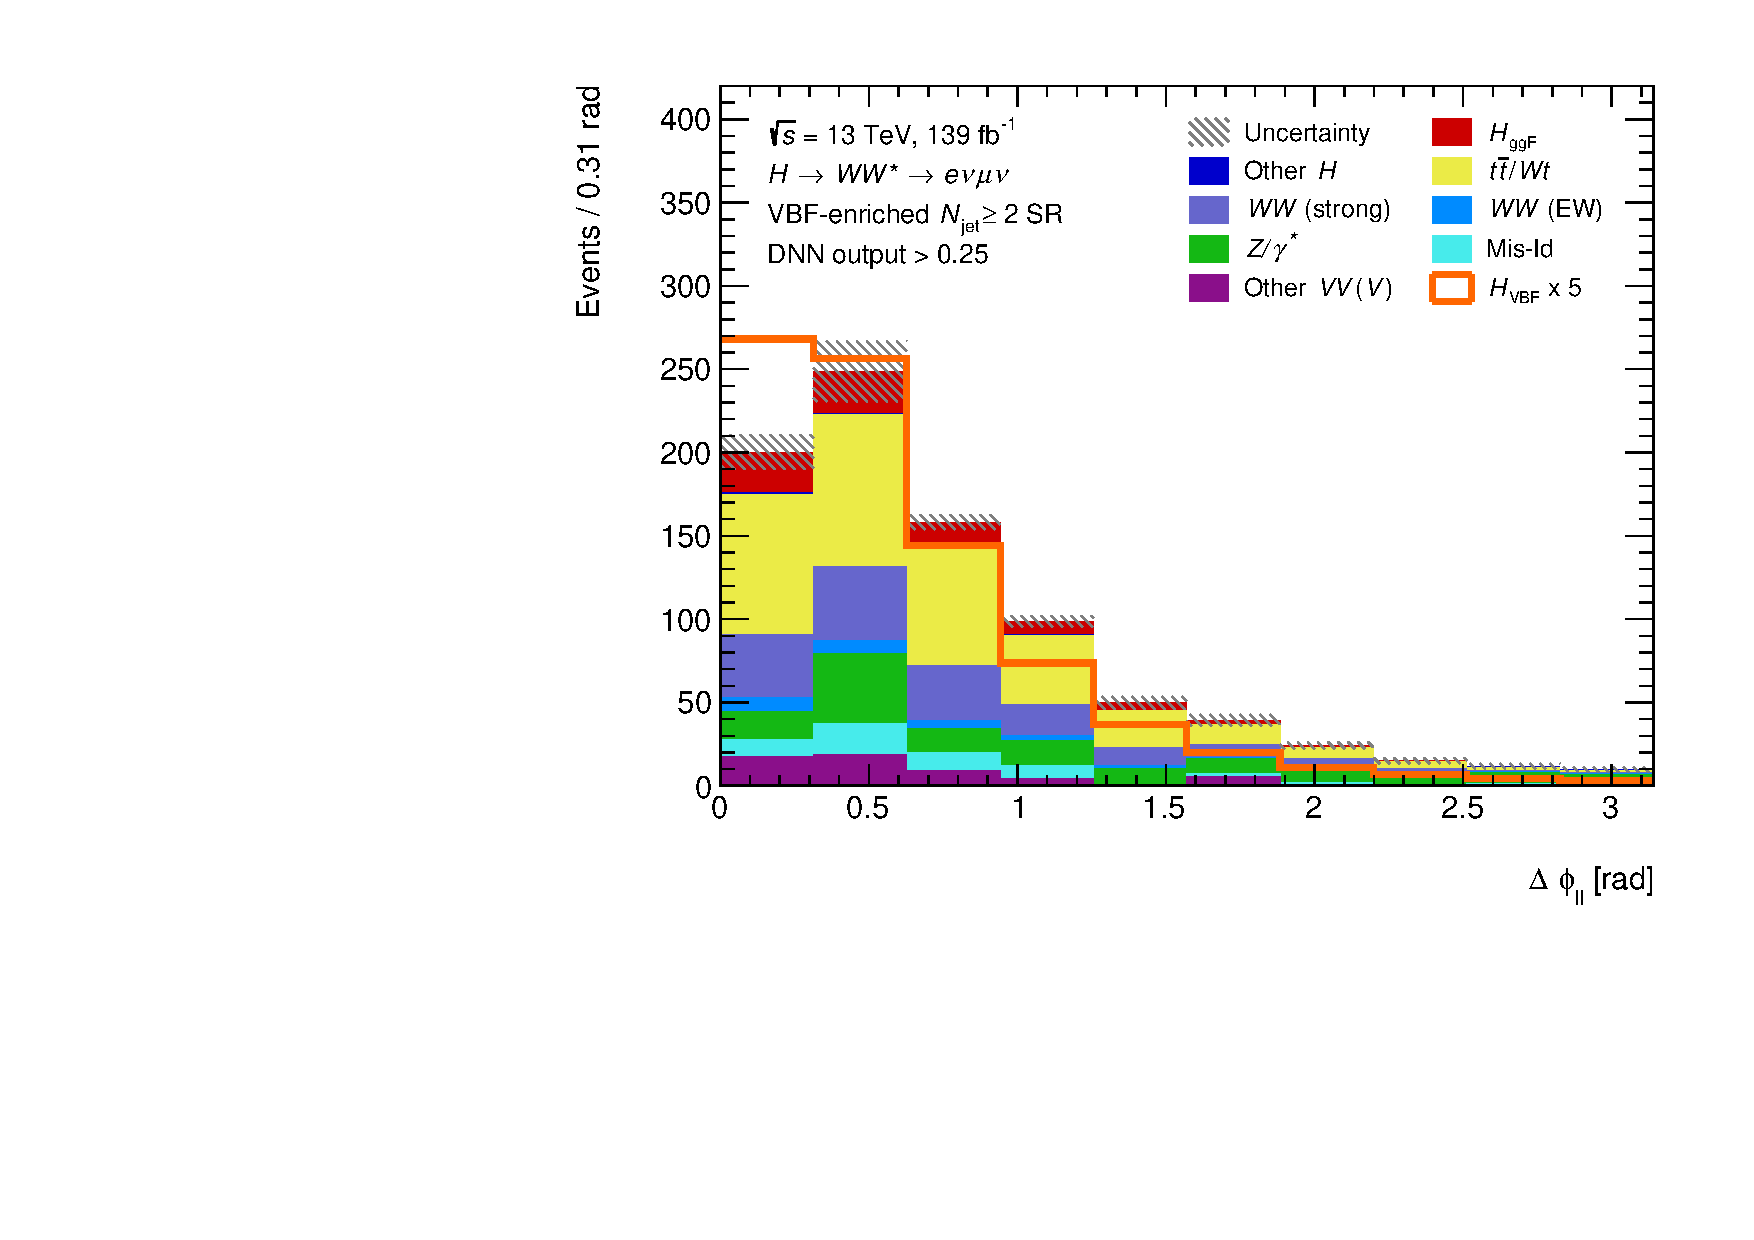
\includegraphics[width=0.32\textwidth]{figures/hww/dnn/blinded/run2-emme-CutVBFSR_DNN25-DPhill-lin.pdf} \hfill
        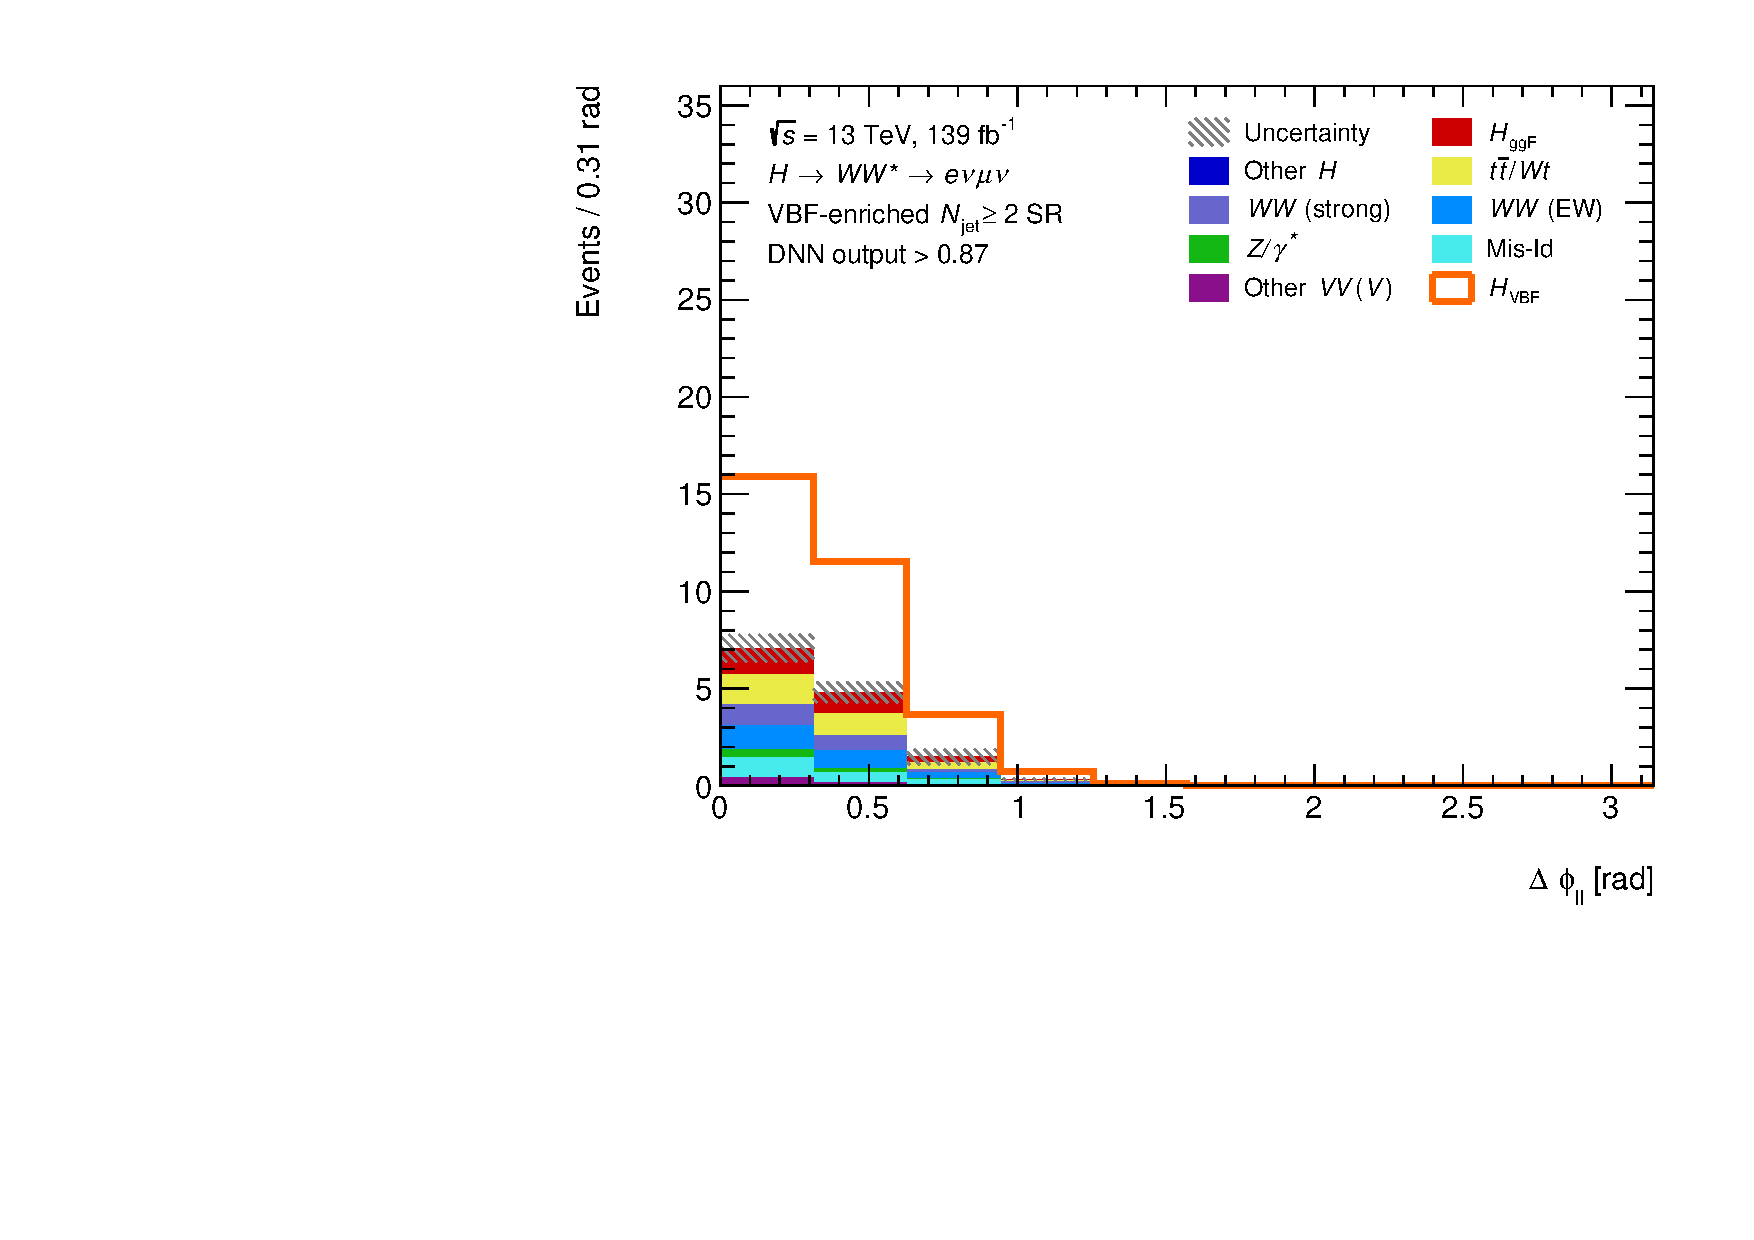
\includegraphics[width=0.32\textwidth]{figures/hww/dnn/blinded/run2-emme-CutVBFSR_DNN87-DPhill-lin.pdf}
    } \\
    \subfloat[$\mll$]{
        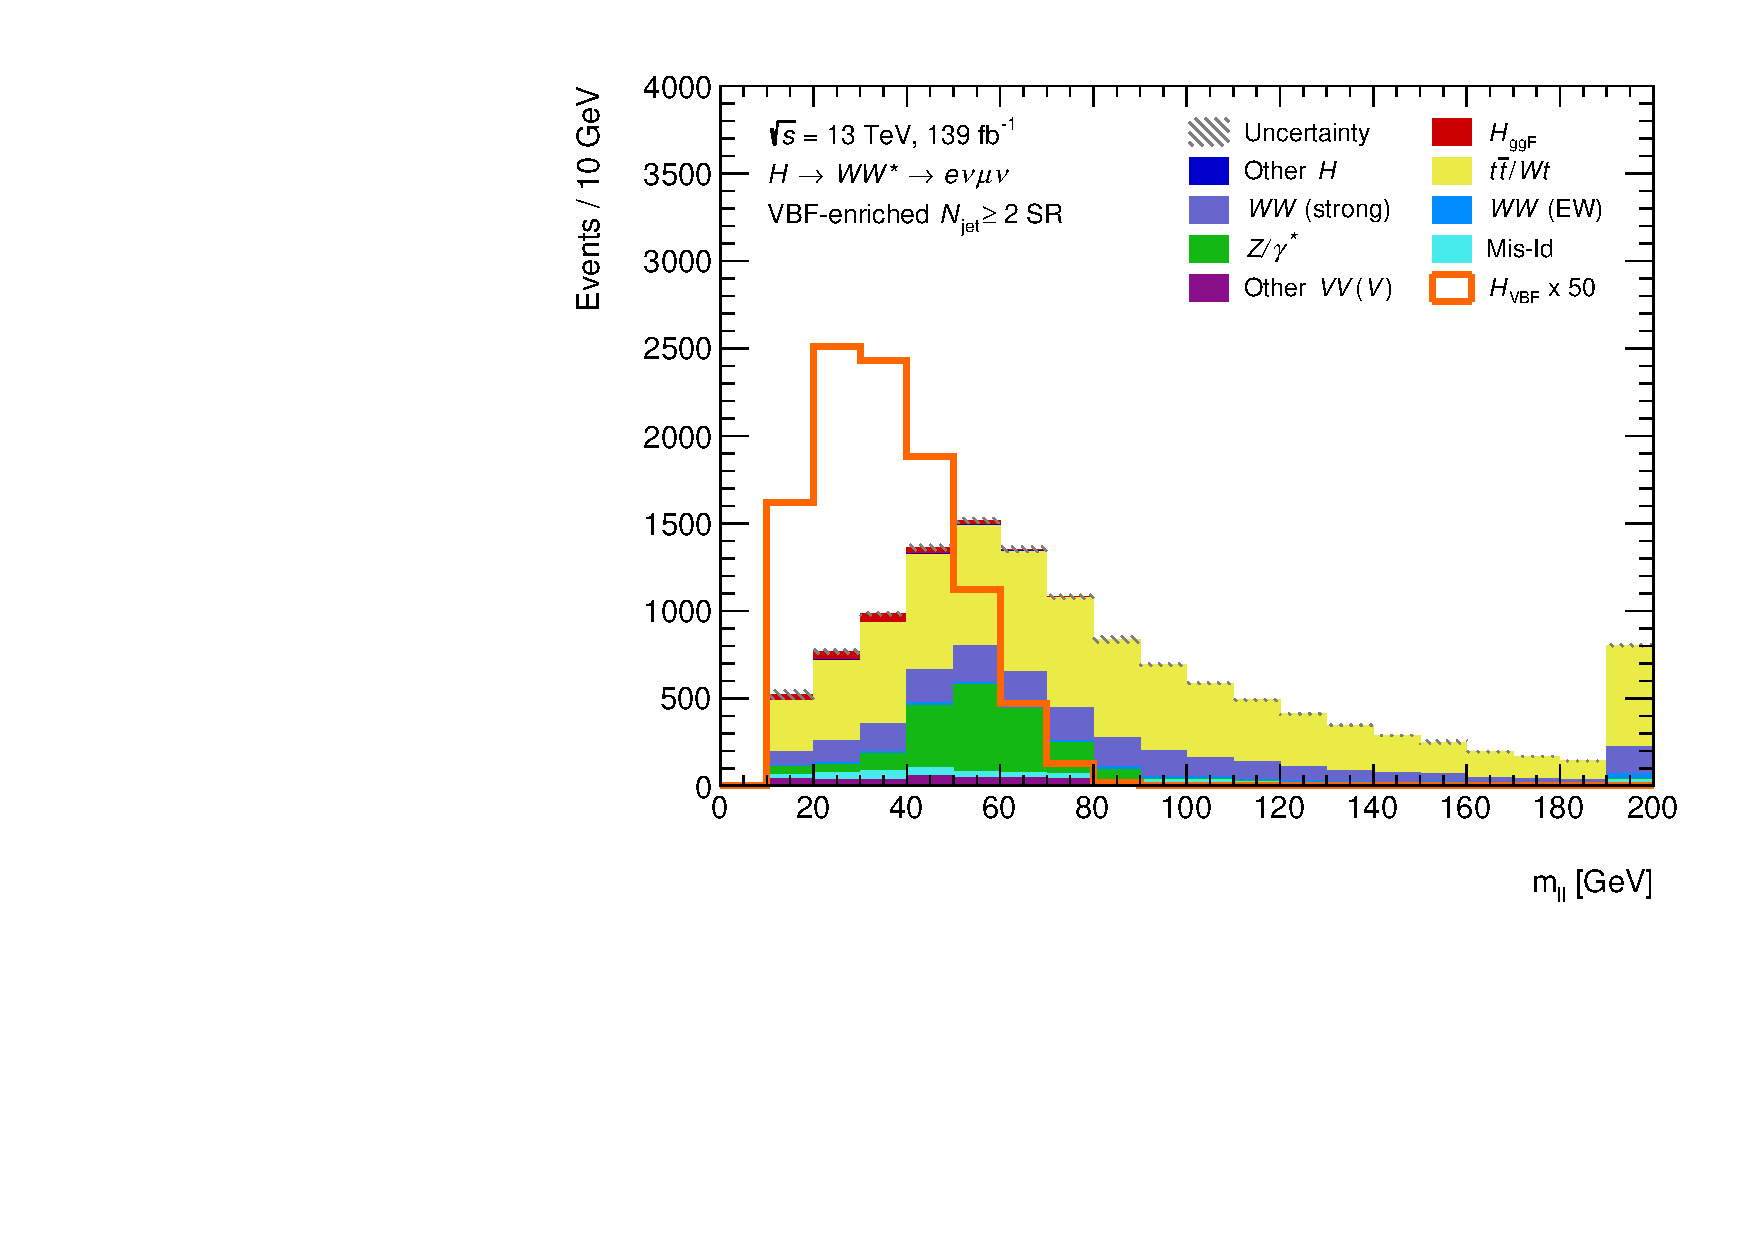
\includegraphics[width=0.32\textwidth]{figures/hww/dnn/blinded/run2-emme-CutVBF_SR-Mll-lin.pdf}
        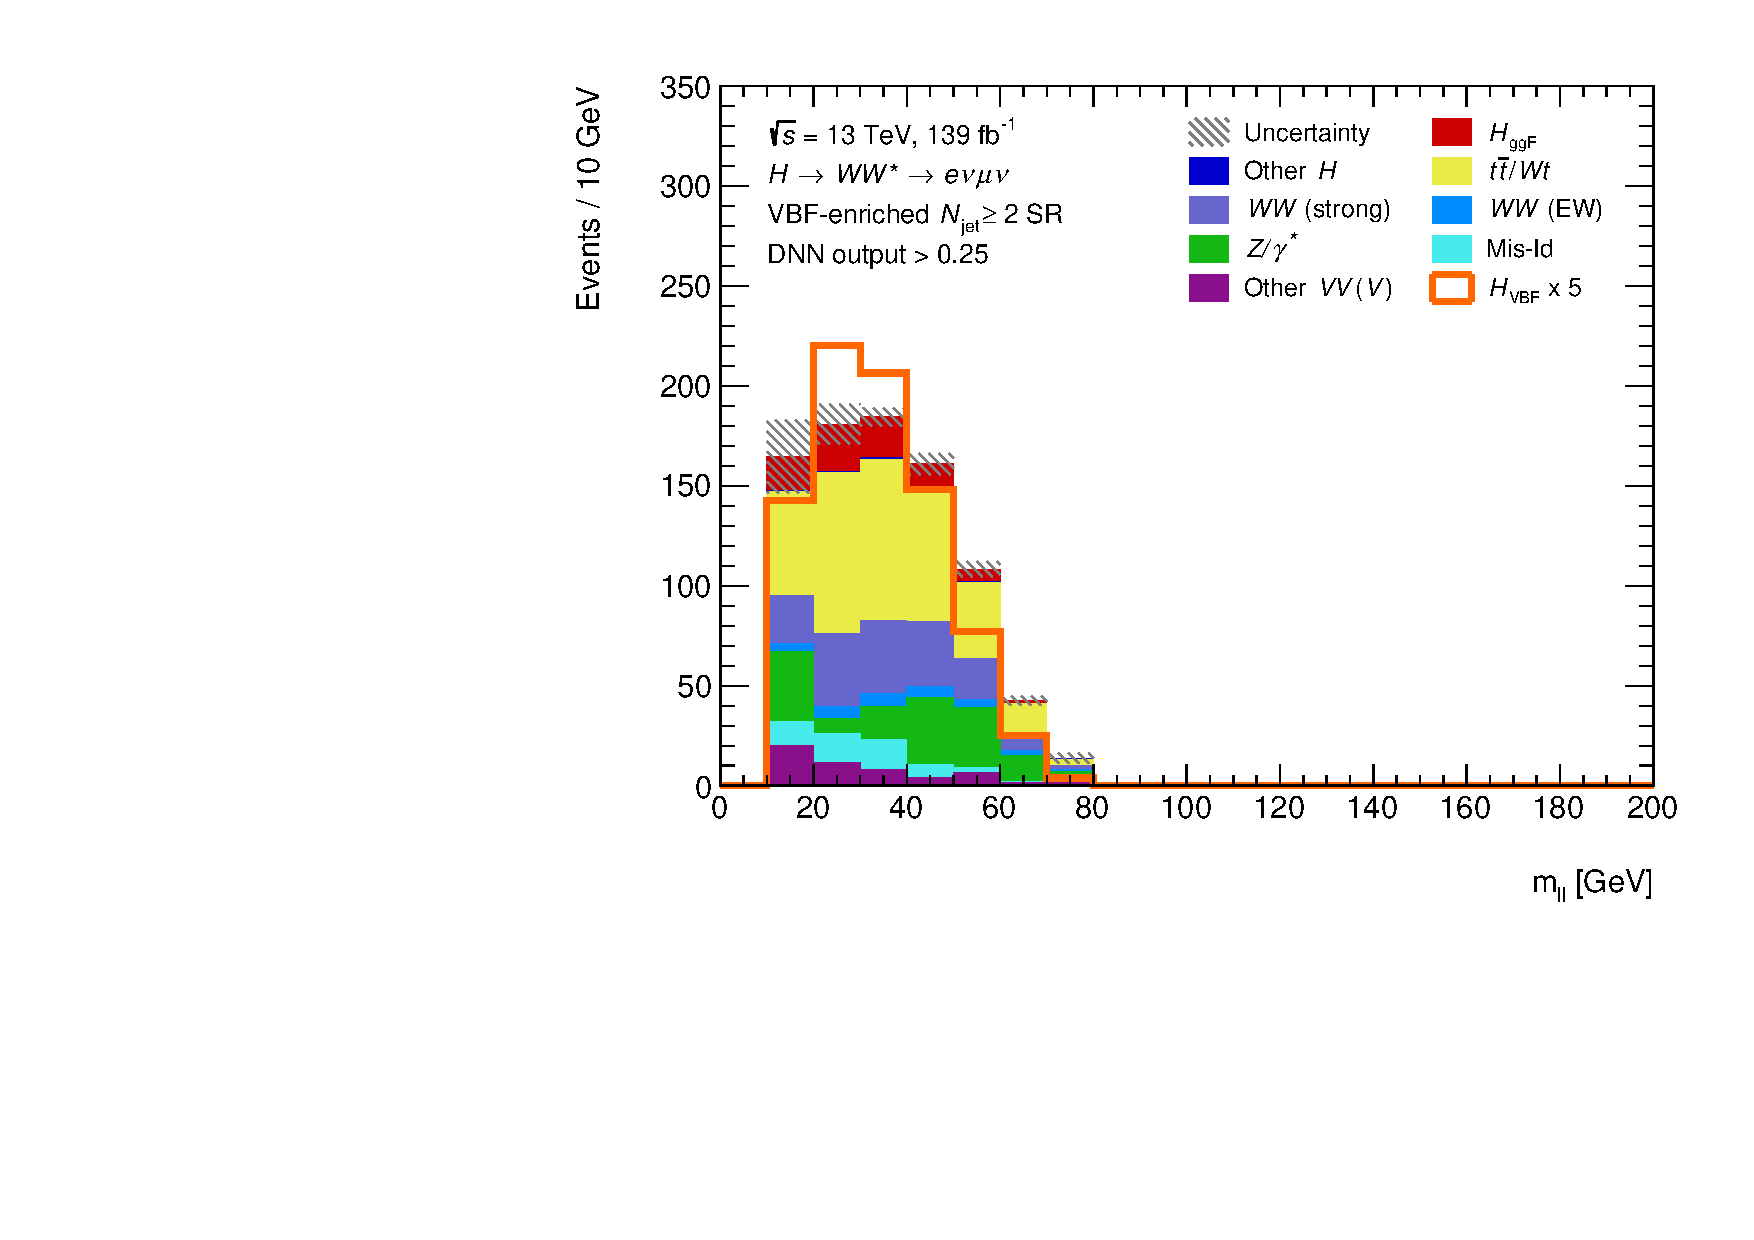
\includegraphics[width=0.32\textwidth]{figures/hww/dnn/blinded/run2-emme-CutVBFSR_DNN25-Mll-lin.pdf}
        \includegraphics[width=0.32\textwidth]{figures/hww/dnn/blinded/run2-emme-CutVBFSR_DNN87-Mll-lin.pdf}
    } \\
    \subfloat[$\mT$]{
        \includegraphics[width=0.32\textwidth]{figures/hww/dnn/blinded/run2-emme-CutVBF_SR-MT-lin.pdf} \hfill
        \includegraphics[width=0.32\textwidth]{figures/hww/dnn/blinded/run2-emme-CutVBFSR_DNN25-MT-lin.pdf} \hfill
        \includegraphics[width=0.32\textwidth]{figures/hww/dnn/blinded/run2-emme-CutVBFSR_DNN87-MT-lin.pdf}
    } 
    {\caption{Distributions of $\dphill$, $\mll$, $\mT$ in the VBF signal region.
        Each row corresponds to one variable with different selections made on the DNN output.
        \label{app:fig:dnn-inputs-hwwdecay} }}
\end{figure}



\begin{figure}[h]
    \centering
    \subfloat[$\pttot$]{
        \includegraphics[width=0.32\textwidth]{figures/hww/dnn/blinded/run2-emme-CutVBF_SR-PtTot-lin.pdf} \hfill
        \includegraphics[width=0.32\textwidth]{figures/hww/dnn/blinded/run2-emme-CutVBFSR_DNN25-PtTot-lin.pdf} \hfill
        \includegraphics[width=0.32\textwidth]{figures/hww/dnn/blinded/run2-emme-CutVBFSR_DNN87-PtTot-lin.pdf}
    } \\
    \subfloat[$\METSig$]{
        \includegraphics[width=0.32\textwidth]{figures/hww/dnn/blinded/run2-emme-CutVBF_SR-METSig_broad-lin.pdf} \hfill
        \includegraphics[width=0.32\textwidth]{figures/hww/dnn/blinded/run2-emme-CutVBFSR_DNN25-METSig_broad-lin.pdf} \hfill
        \includegraphics[width=0.32\textwidth]{figures/hww/dnn/blinded/run2-emme-CutVBFSR_DNN87-METSig_broad-lin.pdf}
    } \\
    {\caption{Distributions of $\pttot$ and $\METSig$ in the VBF signal region.
            Each row shows one variable with different cuts on the DNN output distribution being applied in different columns.
            \label{app:fig:dnn-inputs-top-sup} }}
\end{figure}
}

%%%%%%%%%%%%%%%%%%%%%%%
% Pre-fit Normalization Factors
% From here: https://gitlab.cern.ch/atlas-physics-office/HIGG/ANA-HIGG-2018-47/ANA-HIGG-2018-47-INT1/-/blob/master/sections/STXSAnalysesStrategy-vbf.tex
% \begin{tabular}{c c c}
%     \hline
%     \hline
%      Phase space             &   NF$^\mathrm{\Ztt}$       & NF$^\mathrm{top}$ 	\\
%      \hline
%      \mjjm{350}{700} and \pthle{200}	 & $1.01 \pm 0.06$ &   $1.02 \pm 0.01$				\\
%      \mjjge{700} and \pthle{200}    &   $0.90 \pm 0.10$     & $1.01 \pm 0.03$			\\
%      \mjjge{350} and \pthge{200}   &   $1.04 \pm 0.12$     & $0.94 \pm 0.04$			\\
%     \hline
%     \hline
%     \end{tabular}
%     \caption{Normalisation factors (NF) obtained from the VBF STXS CRs and their uncertainties for the \Ztt and Top backgrounds pre-fit.}
%     \label{tab:vbfstxs:PreNormalisationFactors}
%     \end{table}
    